% Template article for preprint document class `elsart'
% SP 2006/04/26

%\documentclass[seceqn]{elsart}
\documentclass[10pt]{article}

% Package to create index
\usepackage{imakeidx}

% Packages used for html version
%\usepackage{html}

% Packages used for allowing colors
\usepackage{colordvi,color}

% Use the option doublespacing or reviewcopy to obtain double line spacing
%\documentclass[doublespacing,narrowdisplay,draft,seceqn]{elsart}

% if you use PostScript figures in your article
% use the graphics package for simple commands
% \usepackage{graphics}
% or use the graphicx package for more complicated commands
\usepackage{graphicx}
% or use the epsfig package if you prefer to use the old commands
% \usepackage{epsfig}

% The amssymb package provides various useful mathematical symbols
\usepackage{amssymb}

% The lineno packages adds line numbers. Start line numbering with
% \begin{linenumbers}, end it with \end{linenumbers}. Or switch it on
% for the whole article with \linenumbers.
% \usepackage{lineno}

% Package used for forcing the positioning of floating figures
\usepackage{float}

% Package used for allowing multiple columns
\usepackage{multicol}

% Packages with latin1 fonts
\usepackage[utf8]{inputenc}
\makeindex

% Package to make index
%\usepackage{makeidx,showidx}
\usepackage{makeidx}

% Package for hyperlinks
%\usepackage[pdftex=true,colorlinks=true,plainpages=false]{hyperref}
\usepackage[pdftex=true,colorlinks=true,linkcolor=blue]{hyperref}

\usepackage{amsmath}

\usepackage{caption} 
% \graphicspath{{/home/mtaweb/anmol/TOPO2015_mpi/TOPOMANUAL/figs/}} 
\graphicspath{{./figs/}}% para
%poner las gráficas en un subdirectorio

\usepackage{fancyvrb} % Para poner cajas en el texto verbatim 
% Calligraphic letters
\usepackage{calligra,mathrsfs}

\usepackage{showlabels}

%\linenumbers
\topmargin -1cm
\textheight 22cm
\textwidth 16cm
\oddsidemargin 0.5cm
\evensidemargin 0.5cm
\parindent 0pt

\title{User's Guide to DAMQT 3.2.0}
\author{Rafael L\'opez\footnote{Universidad Aut\'onoma de
Madrid,
Facultad de Ciencias. Departamento de Qu\'{i}mica F\'{i}sica Aplicada.}{ },
David Zorrilla\footnote{Universidad de C\'adiz,
Facultad de Ciencias. Departamento de Qu\'{i}mica F\'{i}sica}
and
Anmol Kumar\footnote{Department of Chemistry, Indian Institute of Technology Kanpur, 
Kanpur 208016, India}}

\begin{document}
\renewcommand{\showlabelfont}{\small\slshape\color{red}}
\newcommand{\azul}[1]{{\color{blue}{#1}}}
\newcommand{\llaves}[1]{{\{#1\}}}
\definecolor{negro}{rgb}{0,0,0}
\definecolor{rojo}{rgb}{1.,0,0}
\definecolor{verdeoscuro}{rgb}{.01,.5,0}
\definecolor{naranja}{rgb}{1,.4,.2}
\newcommand{\be}{\begin{equation}}
\newcommand{\ee}{\end{equation}}
\newcommand{\ba}{\begin{array}}
\newcommand{\ea}{\end{array}}
\newcommand{\baa}{\begin{eqnarray}}
\newcommand{\eaa}{\end{eqnarray}}
\newcommand{\rne}{{\bf r}}
\newcommand{\Rne}{{\bf R}}
\newcommand{\Ene}{{\bf E}}
\newcommand{\Fne}{{\bf F}}
\newcommand{\Sne}{{\bf S}}
\newcommand{\Acal}{\mathscr{A}}
\newcommand{\Vcal}{\mathscr{V}}
\newcommand{\aux}{{\it .aux}}
\newcommand{\basis}{{\it .basis}}
\newcommand{\bmp}{{\it .bmp}}
\newcommand{\cam}{{\it .cam}}
\newcommand{\camdosD}{{\it .cam2D}}
\newcommand{\chk}{{\it .chk}}
\newcommand{\cnt}{{\it .cnt}}
\newcommand{\com}{{\it .com}}
\newcommand{\control}{{\it .control}}
\newcommand{\coords}{{\it .coords}}
\newcommand{\cplt}{{\it cxx-d.plt}}
\newcommand{\damproj}{{\it .damproj}}
\newcommand{\damqt}{{\it \_2016.damqt}}
\newcommand{\dmqtv}{{\it \_2016.dmqtv}}
\newcommand{\den}{{\it .den}}
\newcommand{\dengr}{{\it .dengr}}
\newcommand{\dengrdosD}{{\it .dengr2D}}
\newcommand{\dengz}{{\it .den.gz}}
\newcommand{\dplt}{{\it -d.pltd}}
\newcommand{\fcf}{{\it .fcf}}
\newcommand{\fchk}{{\it .fchk}}
\newcommand{\fnc}{{\it .fnc}}
\newcommand{\formchk}{{\it .formchk}}
\newcommand{\frad}{{\it .frad}}
\newcommand{\fre}{{\it .fre}}
\newcommand{\frgplt}{{\it frg-d.plt}}
\newcommand{\fri}{{\it .fri}}
\newcommand{\frt}{{\it .frt}}
\newcommand{\ggbs}{{\it .ggbs}}
\newcommand{\gnu}{{\it .gnu}}
\newcommand{\inp}{{\it .inp}}
\newcommand{\jpg}{{\it .jpg}}
\newcommand{\jpeg}{{\it .jpeg}}
\newcommand{\mkl}{{\it .mkl}}
\newcommand{\mos}{{\it .mos}}
\newcommand{\nwcout}{{\it .nwcout}}
\newcommand{\out}{{\it .out}}
\newcommand{\png}{{\it .png}}
\newcommand{\ppm}{{\it .ppm}}
\newcommand{\plt}{{\it .plt}}
\newcommand{\pltd}{{\it .pltd}}
\newcommand{\sgbs}{{\it .sgbs}}
\newcommand{\sgh}{{\it .sgh}}
\newcommand{\tiff}{{\it .tiff}}
\newcommand{\xml}{{\it .xml}}
\newcommand{\xpm}{{\it .xpm}}
\newcommand{\xbm}{{\it .xbm}}
\newcommand{\xyz}{{\it .xyz}}

\newcommand{\tttmake}{\texttt{make }}
\newcommand{\tttmakeinstall}{\texttt{make install }}
\newcommand{\tttconfigure}{\texttt{./configure }}
\newcommand{\tttshconfigure}{\texttt{sh ./configure }}

\newcommand{\teclapuntos}{
\begin{minipage}[t][1mm][t]{.35cm}{
\vspace*{-8pt}
\includegraphics[width=.35cm]{3dots.png}}
\end{minipage}
}
\newcommand{\exec}{
\begin{minipage}[t][1mm][t]{.7cm}{
\vspace*{-8pt}
\includegraphics[width=.7cm]{exec.png} }
\end{minipage}
}
\newcommand{\add}{
\begin{minipage}[t][1mm][t]{.35cm}{
\vspace*{-8pt}
\includegraphics[width=.35cm]{add.png} }
\end{minipage}
}
\newcommand{\remove}{
\begin{minipage}[t][1mm][t]{.35cm}{
\vspace*{-8pt}
\includegraphics[width=.35cm]{remove.png} }
\end{minipage}
}
\newcommand{\listados}{
\begin{minipage}[t][1mm][t]{.35cm}{
\vspace*{-8pt}
\includegraphics[width=.35cm]{listados.png} }
\end{minipage}
}
\newcommand{\reset}{
\begin{minipage}[t][1mm][t]{.7cm}{
\includegraphics[width=.7cm]{reset.png} }
\end{minipage}
}
\newcommand{\start}{
\begin{minipage}[t][1mm][t]{.7cm}{
\includegraphics[width=.7cm]{start.png} }
\end{minipage}
}
\newcommand{\stopkeya}{
\begin{minipage}[t][1mm][t]{.7cm}{
\vspace*{-8pt}
\includegraphics[width=.7cm]{stop1.png} }
\end{minipage}
}
\newcommand{\stopkeyb}{
\begin{minipage}[t][1mm][t]{.7cm}{
\includegraphics[width=.7cm]{stop2.png} }
\end{minipage}
}
\newcommand{\colorkey}{
\begin{minipage}[t][1mm][t]{.7cm}{
\includegraphics[width=.7cm]{colorkey.png} }
\end{minipage}
}
\newcommand{\fontkey}{
\begin{minipage}[t][1mm][t]{.7cm}{
\includegraphics[width=.7cm]{fontkey.png} }
\end{minipage}
}
\newcommand{\minuskey}{
\begin{minipage}[t][1mm][t]{.35cm}{
\vspace*{-8pt}
\includegraphics[width=.35cm]{minuskey.png} }
\end{minipage}
}
\newcommand{\pluskey}{
\begin{minipage}[t][1mm][t]{.35cm}{
\vspace*{-8pt}
\includegraphics[width=.35cm]{pluskey.png} }
\end{minipage}
}
\newcommand{\update}{
\begin{minipage}[t][1mm][t]{.7cm}{
\includegraphics[width=.7cm]{update.png} }
\end{minipage}
}
\newcommand{\toolbN}{
\begin{minipage}[t][1mm][t]{.35cm}{
\vspace*{-8pt}
\includegraphics[width=.35cm]{toolb1.png}}
\end{minipage}
}
\newcommand{\toolbA}{
\begin{minipage}[t][1mm][t]{.35cm}{
\vspace*{-8pt}
\includegraphics[width=.35cm]{toolb2.png}}
\end{minipage}
}
\newcommand{\toolbS}{
\begin{minipage}[t][1mm][t]{.35cm}{
\vspace*{-8pt}
\includegraphics[width=.35cm]{toolb3.png}}
\end{minipage}
}
\newcommand{\toolbP}{
\begin{minipage}[t][1mm][t]{.35cm}{
\vspace*{-8pt}
\includegraphics[width=.35cm]{toolb4.png}}
\end{minipage}
}
\newcommand{\toolbD}{
\begin{minipage}[t][1mm][t]{.35cm}{
\vspace*{-8pt}
\includegraphics[width=.35cm]{toolb5.png}}
\end{minipage}
}
\newcommand{\toolbC}{
\begin{minipage}[t][1mm][t]{.35cm}{
\vspace*{-8pt}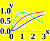
\includegraphics[width=.35cm]{toolb6.png}}
\end{minipage}
}
\newcommand{\toolbV}{
\begin{minipage}[t][1mm][t]{.35cm}{
\vspace*{-8pt}
\includegraphics[width=.35cm]{toolb7.png}}
\end{minipage}
}
\newcommand{\toolbH}{
\begin{minipage}[t][1mm][t]{.35cm}{
\vspace*{-8pt}
\includegraphics[width=.35cm]{toolb8.png}}
\end{minipage}
}
\newcommand{\toolbB}{
\begin{minipage}[t][1mm][t]{.35cm}{
\vspace*{-8pt}
\includegraphics[width=.35cm]{toolb9.png}}
\end{minipage}
}
\newcommand{\toolbQ}{
\begin{minipage}[t][1mm][t]{.35cm}{
\vspace*{-8pt}
\includegraphics[width=.35cm]{toolb10.png}}
\end{minipage}
}
\newcommand{\toolbE}{
\begin{minipage}[t][1mm][t]{.35cm}{
\vspace*{-8pt}
\includegraphics[width=.35cm]{toolb11.png}}
\end{minipage}
}
\newcommand{\bigtoolbN}{
\begin{minipage}[t][1mm][t]{.5cm}{
\vspace*{-8pt}
\includegraphics[width=.5cm]{toolb1.png}}
\end{minipage}
}
\newcommand{\bigtoolbA}{
\begin{minipage}[t][1mm][t]{.5cm}{
\vspace*{-8pt}
\includegraphics[width=.5cm]{toolb2.png}}
\end{minipage}
}
\newcommand{\bigtoolbS}{
\begin{minipage}[t][1mm][t]{.5cm}{
\vspace*{-8pt}
\includegraphics[width=.5cm]{toolb3.png}}
\end{minipage}
}
\newcommand{\bigtoolbP}{
\begin{minipage}[t][1mm][t]{.5cm}{
\vspace*{-8pt}
\includegraphics[width=.5cm]{toolb4.png}}
\end{minipage}
}
\newcommand{\bigtoolbD}{
\begin{minipage}[t][1mm][t]{.5cm}{
\vspace*{-8pt}
\includegraphics[width=.5cm]{toolb5.png}}
\end{minipage}
}
\newcommand{\bigtoolbC}{
\begin{minipage}[t][1mm][t]{.5cm}{
\vspace*{-8pt}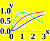
\includegraphics[width=.5cm]{toolb6.png}}
\end{minipage}
}
\newcommand{\bigtoolbV}{
\begin{minipage}[t][1mm][t]{.5cm}{
\vspace*{-8pt}
\includegraphics[width=.5cm]{toolb7.png}}
\end{minipage}
}
\newcommand{\bigtoolbH}{
\begin{minipage}[t][1mm][t]{.5cm}{
\vspace*{-8pt}
\includegraphics[width=.5cm]{toolb8.png}}
\end{minipage}
}
\newcommand{\bigtoolbB}{
\begin{minipage}[t][1mm][t]{.5cm}{
\vspace*{-8pt}
\includegraphics[width=.5cm]{toolb9.png}}
\end{minipage}
}
\newcommand{\bigtoolbQ}{
\begin{minipage}[t][1mm][t]{.5cm}{
\vspace*{-8pt}
\includegraphics[width=.5cm]{toolb10.png}}
\end{minipage}
}
\newcommand{\bigtoolbE}{
\begin{minipage}[t][1mm][t]{.5cm}{
\vspace*{-8pt}
\includegraphics[width=.5cm]{toolb11.png}}
\end{minipage}
}
\newcommand{\undock}{
\begin{minipage}[t][1mm][t]{.3cm}{
\vspace*{-8pt}
\includegraphics[width=.3cm]{undock.png}}
\end{minipage}
}
\newcommand{\zoomin}{
\begin{minipage}[t][1mm][t]{.3cm}{
\vspace*{-8pt}
\includegraphics[width=.3cm]{zoom_in.png}}
\end{minipage}
}
\newcommand{\zoomout}{
\begin{minipage}[t][1mm][t]{.3cm}{
\vspace*{-8pt}
\includegraphics[width=.3cm]{zoom_out.png}}
\end{minipage}
}

\newenvironment{rcase}{
\left.\begin{aligned}}
  {\end{aligned}\right\rbrace
}
\newenvironment{lcase}{
\left\lbrace\begin{aligned}}
  {\end{aligned}\right.
}

\maketitle
\vspace{\stretch{.5}}

\newpage

\tableofcontents


\pagebreak

\section*{DAMQT 3.2.0 \label{sec:0}}
DAMQT is a software package designed for the analysis and visualization of molecular electron density (MED) in atoms and molecules, along with several related properties such as density deformations, electrostatic potential, molecular topography, sigma holes, electric field, Hellmann-Feynman forces, molecular orbitals, and density fingerprints using Zernike-Canterakis and Jacobi functions. Additionally, cluster optimization for non-bonding interacting systems has recently been integrated into the package.

The method implemented in DAMQT is based on the DAM partition of electron density into atomic fragments using a least deformation criterion, as described elsewhere\footnote{For a description of the
fundamentals, see for instance, J. Fern\'andez Rico, et al. Comput. Chem. 25
(2004) 1355; J. Mol. Struct. Theochem 727 (2005) 115, and the references
included in these articles}. Density fingerprints are computed as expansions of Zernike-Canterakis or Jacobi functions within a user-defined spherical region, employing translation techniques for Slater or Gaussian basis functions\footnote{For details see G. Urquiza-Carvalho et al. J. Comput. Chem. 39 (2018) 2022}. Cluster optimization is performed using the EPIC procedure (Gadre S, Babu K, Resonance 4 (1999) 40).

In the DAM partition, the electron density of each atomic fragment is expanded in terms of radial functions multiplied by regular spherical harmonics centered at its nucleus. As a result, the electron density of the entire molecule is represented as a set of atomic expansions in terms of effective multipoles, which are functions of the distance to their corresponding nuclei.

The radial components of the effective multipoles are expanded in a piecewise manner using exponentials multiplied by polynomials of the radial variable $r$. This representation enables the efficient computation of the molecular electrostatic potential (MESP) and electric field generated by both the electron density and the nuclei, as well as the calculation of Hellmann-Feynman forces acting on the nuclei. Additionally, the molecular topography of MED and MESP, as well as atomic and molecular density deformations, can be visualized, offering insights that connect with various empirical concepts in structural chemistry.

DAMQT follows a modular three-level structure (see fig \ref{fig:1}), , with interfaces to standard quantum mechanical calculation packages integrated at the top level. While an interface for ADF is included in the suite, it is also provided within DAMQT for completeness. The package currently supports interfaces to MOLPRO, GAUSSIAN, MOPAC, TURBOMOLE, and NWCHEM, along with a feature for reading MOLEKEL \mkl{ } files.

\begin{figure}[H]
% \hspace*{-0.5cm}
\vspace*{-2cm}
\begin{center}
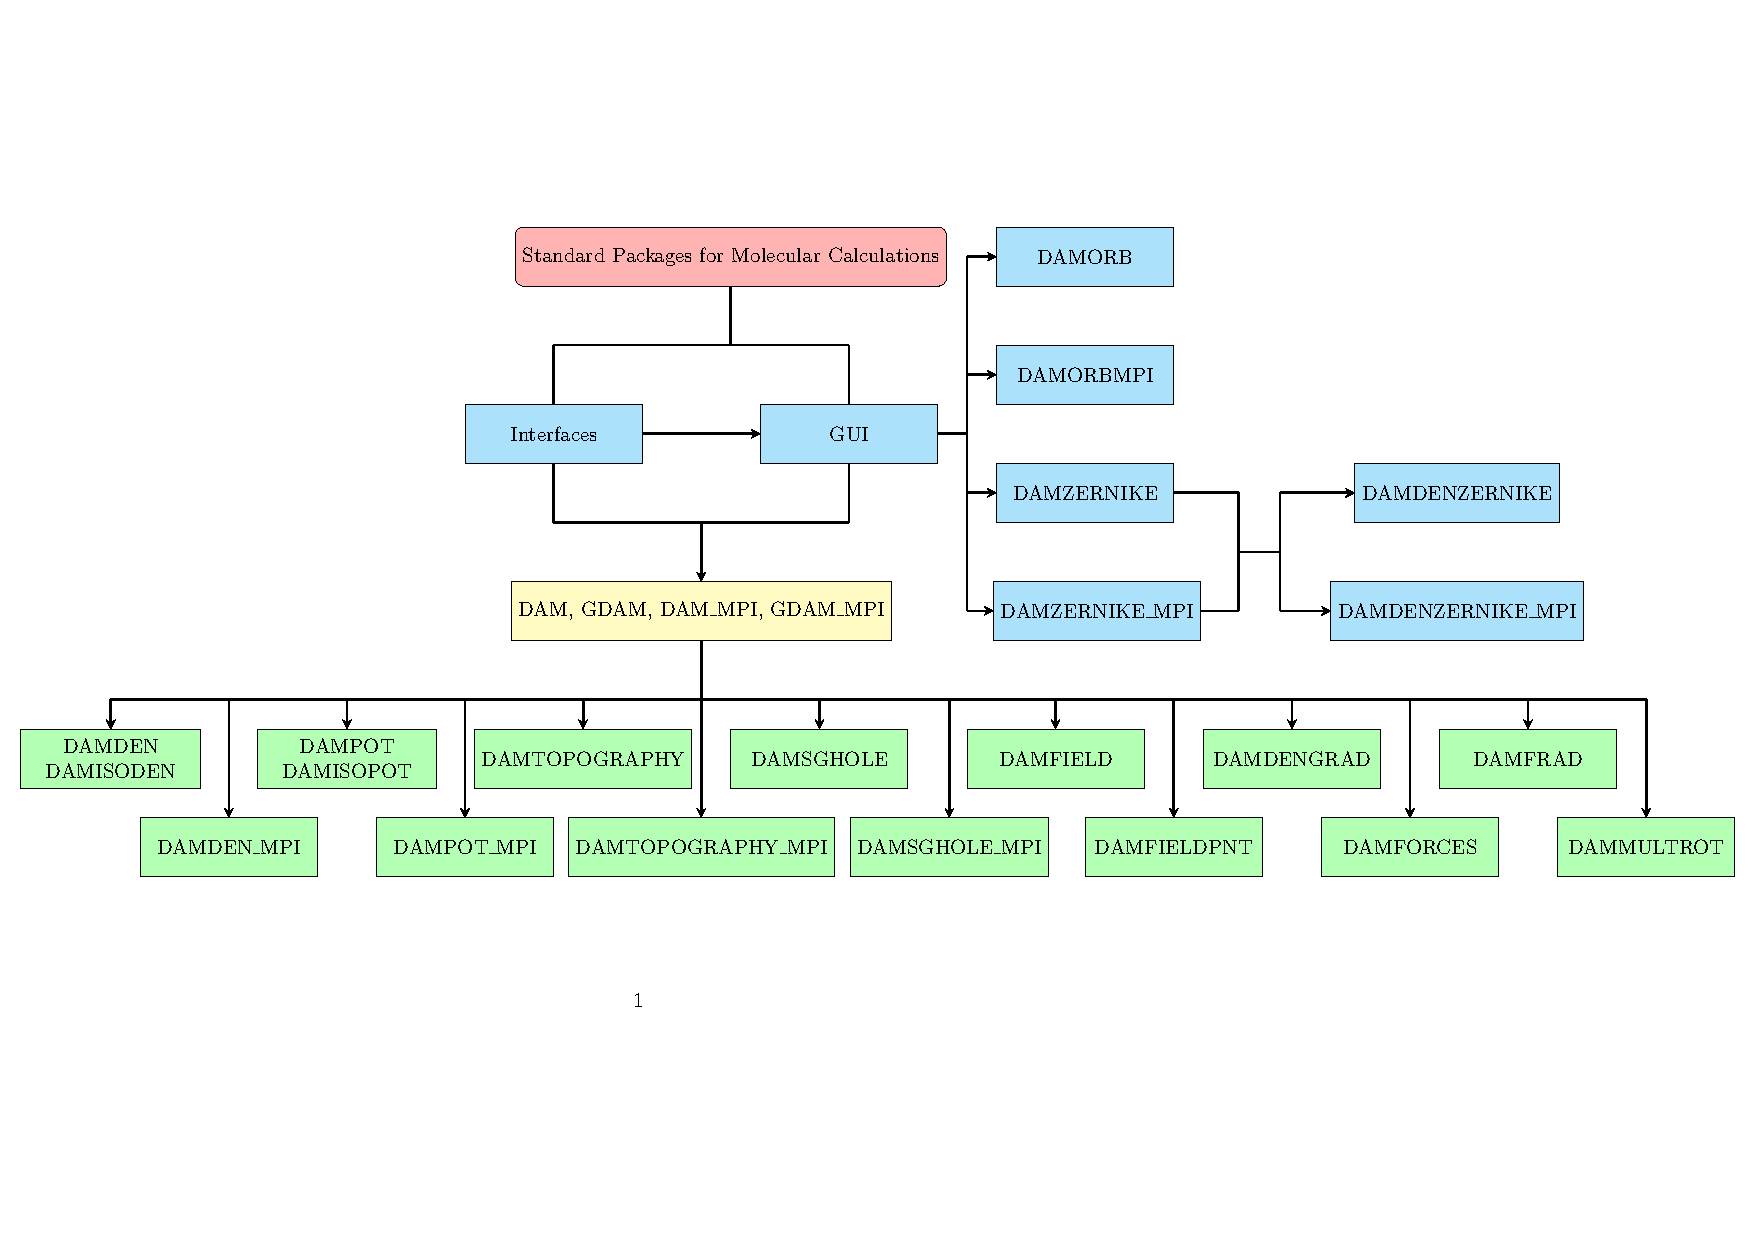
\includegraphics[width=1\linewidth]{DAMQT_structure.pdf}
\end{center}
\vspace*{-2.5cm}
\caption{DAMQT structure \label{fig:1}}
\end{figure}

At this level, DAMQT also includes the GUI\index{GUI}, designed to enhance usability.
This GUI is written in C++ and developed using the Qt library\footnote{The Qt Company, www.qt.io}, ensuring portability across different operating systems. Additionally, this level provides programs for generating molecular orbital grids for 2D plotting and 3D visualization within the GUI.

Programs for Zernike-Canterakis or Jacobi expansions of MED and their corresponding grid generation for plotting are also included here.
These programs can be executed directly from the GUI without requiring the partition/expansion of MED.

Furthermore, cluster optimization via the EPIC procedure (MESPIMIZER) is integrated into the 3D viewer. However, this feature requires the DAM partition/expansion for the host molecule. 

The second level comprises programs responsible for DAM partition/expansion of electron density for Gaussian and Slater densities.

These programs are available for both scalar and parallel computation with MPI.
One of these programs must be executed before accessing those in the third level, as the latter requires the partition/expansion data generated by the former. 

Finally, the bottom level contains a variety of programs for computing multiple properties using the DAM partition/expansion. 

In particular, this expansion enables the efficient computation of electron density and its deformations, electrostatic potential, electric field, density gradient,
molecular topography of electron density and electrostatic potential, sigma holes, and Hellmann-Feynman forces on nuclei.

Unless explicitly stated otherwise, atomic units will be used throughout this document.

\newpage

\section{Installation \label{sec:1}}

DAMQT 3.2.0 is available for Linux and MS Windows under GNU's GPL license.
The package includes both the source code and other ancillary files.
The sources can be modified and distributed in accordance with the terms of GPLv3.

The minimum system requirements for installation are 200MB of RAM and 150MB of disk storage.
However, memory requirements depend significantly on the size of the systems being processed.
Additionally, access to Fortran 90 and C++ compilers, as well as a Python interpreter, is required.

For the Linux version, the following dependencies must be installed:
\begin{itemize}
\item Qt-project's Qt library (version 5.9 or higher, including development libraries)
\item OpenGL 3.3 or higher
\end{itemize}

For cluster optimization using OpenBabel atom charges, \texttt{OpenBabel} is required.

To create movies from captures, \texttt{ffmpeg} may also be necessary.

\subsection{Linux and MacOS installation \label{sec:1.1}\index{installation!linux}}

\texttt{DAM\_3.2.0} is distributed as a tarball
({\it DAM\_3.2.0\_}\texttt{datestamp}{\it .tar.gz}),
where $\texttt{datestamp}$ represents an eight-digit date in the format \texttt{yyyymmdd}.

To install DAMQT on Linux, Unix, or macOS, navigate to a suitable directory and copy the file
{\it DAM\_3.2.0\_}\texttt{datestamp}{\it .tar.gz} there. Then, extract its contents using:
\begin{verbatim}
tar -vxzf DAM_3.2.0_datestamp.tar.gz
\end{verbatim}

This will create a directory named \texttt{DAM\_3.2.0}, which contains the source files and ancillary components.
\texttt{DAM\_3.2.0} is designed to be installed using \texttt{cmake}.
Before proceeding, ensure that \texttt{cmake} is available on your system.
For ease of configuration, the \texttt{cmake-gui} graphical interface is highly recommended, as it simplifies variable management.

To prevent cmake from placing generated files directly in the DAMQT source directory,
it is strongly recommended to create a separate directory for the installation process.

For installation via \texttt{cmake} from the command line, navigate to the desired installation directory and execute one of the following commands:

\begin{itemize}
\item {\bf Basic installation:}

\begin{verbatim}
cmake {\it damdir}
\end{verbatim}
%
where \texttt{damdir} is the root directory of DAMQT.

\item {\bf Interactive installation with customization options:}

\begin{verbatim}
cmake -i
\end{verbatim}

By default, running \texttt{make install}\footnote{You may need root privileges for this step.} will install the package files in:
\vspace*{-5mm}
\begin{quote}
\item \texttt{/usr/local/bin}
\item \texttt{/usr/local/man}, etc.
\end{quote}

To install the package in a different location, set the \texttt{cmake} variable \texttt{CMAKE\_INSTALL\_PREFIX} to the desired {\it path}.
{\bf WARNING:} Avoid using blank spaces in the installation path.

Additional installation options can be customized by modifying the appropriate \texttt{cmake} variables.

\item {\bf Uninstallation\index{uninstallation!linux}}

The package can be removed using:

\begin{verbatim}
make uninstall
\end{verbatim}

\item {\bf Special Notes for OpenGL with MESA\index{MESA}}


On certain systems, if the MESA library is used for OpenGL,
it may be necessary to run the following command before launching DAMQT:

\begin{verbatim}
MESA_GL_VERSION_OVERRIDE=4.5 MESA_GLSL_VERSION_OVERRIDE=450 path_to_DAMQT
\end{verbatim}

If a version other than 4.5 (but $\ge 3.3$) is required, modify both 4.5 and 450 accordingly.

\end{itemize}

\subsection{Windows installation \label{sec:1.2}\index{installation!windows}}

The MS-Windows version can also be installed using \texttt{cmake}, but an autoinstall file,
{\it DAMQT\_3.2.0\_setup.exe}, is provided with the package. Simply click on this file and follow the installation instructions.

The Samples folder will be installed in the {\it AppData/Local} directory.

To prevent unintended data loss, this folder will not be removed when uninstalling DAMQT.
If necessary, it must be deleted manually.

To enable cluster optimization using OpenBabel atom charges, the \texttt{OpenBabel} package must be installed,
and its executable must be accessible. To ensure this:

\begin{itemize}
\item Include the directory containing the OpenBabel executable in the user's \texttt{PATH}.
\item Verify that the \texttt{BABEL\_DATADIR} variable is set in the user's environment variables.
\item Ensure that \texttt{BABEL\_DATADIR} points to the correct folder, where the {\it qeq.txt} file must be present.
\end{itemize}

It is essential that \texttt{OpenBabel} is installed and its environment variables are set
before launching DAMQT for cluster optimization. Otherwise, the executable or its auxiliary files may not be found,
leading to potential optimization failures.

To create movies from captures, ensure that \texttt{ffmpeg} or another suitable program is accessible
by including the relevant folder in the user's \texttt{PATH} variable.

\subsection{Starting DAMQT \label{sec:1.3}\index{installation!starting DAMQT}}


\begin{minipage}{.65\linewidth}

To start DAMQT, open a {\it console} (UNIX/Linux/MacOS), type \texttt{DAMQT320.exe}, and press {\it enter}.

For MS-Windows, the installer provides the option to create a desktop icon for direct access.
Alternatively, you can manually run DAMQT320.exe from the installation folder.

A pop-up window will appear over a splash image (fig \ref{fig:1_3_1}),
prompting you to select a language. Choose your preferred option and click the {\it Start} button.
The splash image will glow while DAMQT initializes. Once it disappears, DAMQT is ready to use.

\end{minipage}
\begin{minipage}{.38\linewidth}
\vspace*{-8mm}
\begin{figure}[H]
\begin{center}
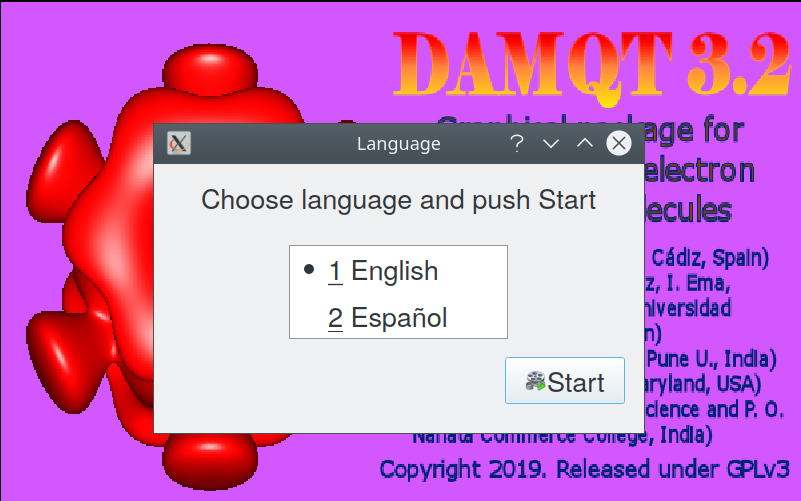
\includegraphics[width=.83\linewidth]{damqt320_splash.png}
\end{center}
\caption{{Starting window}\label{fig:1_3_1}}
\end{figure}
\end{minipage}

\newpage

\section{The Graphical User Interface I: Main window \label{sec:2}\index{main
window}}

The GUI follows a standard design, featuring:

\begin{itemize}
\item A menu bar and toolbar at the top,
\item An application driving menu on the left,
\item A display area for standard application outputs, and
\item A menu on the right for managing graphical viewers (fig. \ref{fig:2_1}).
\end{itemize}

\vspace*{0cm}
\begin{figure}[H]
\begin{center}
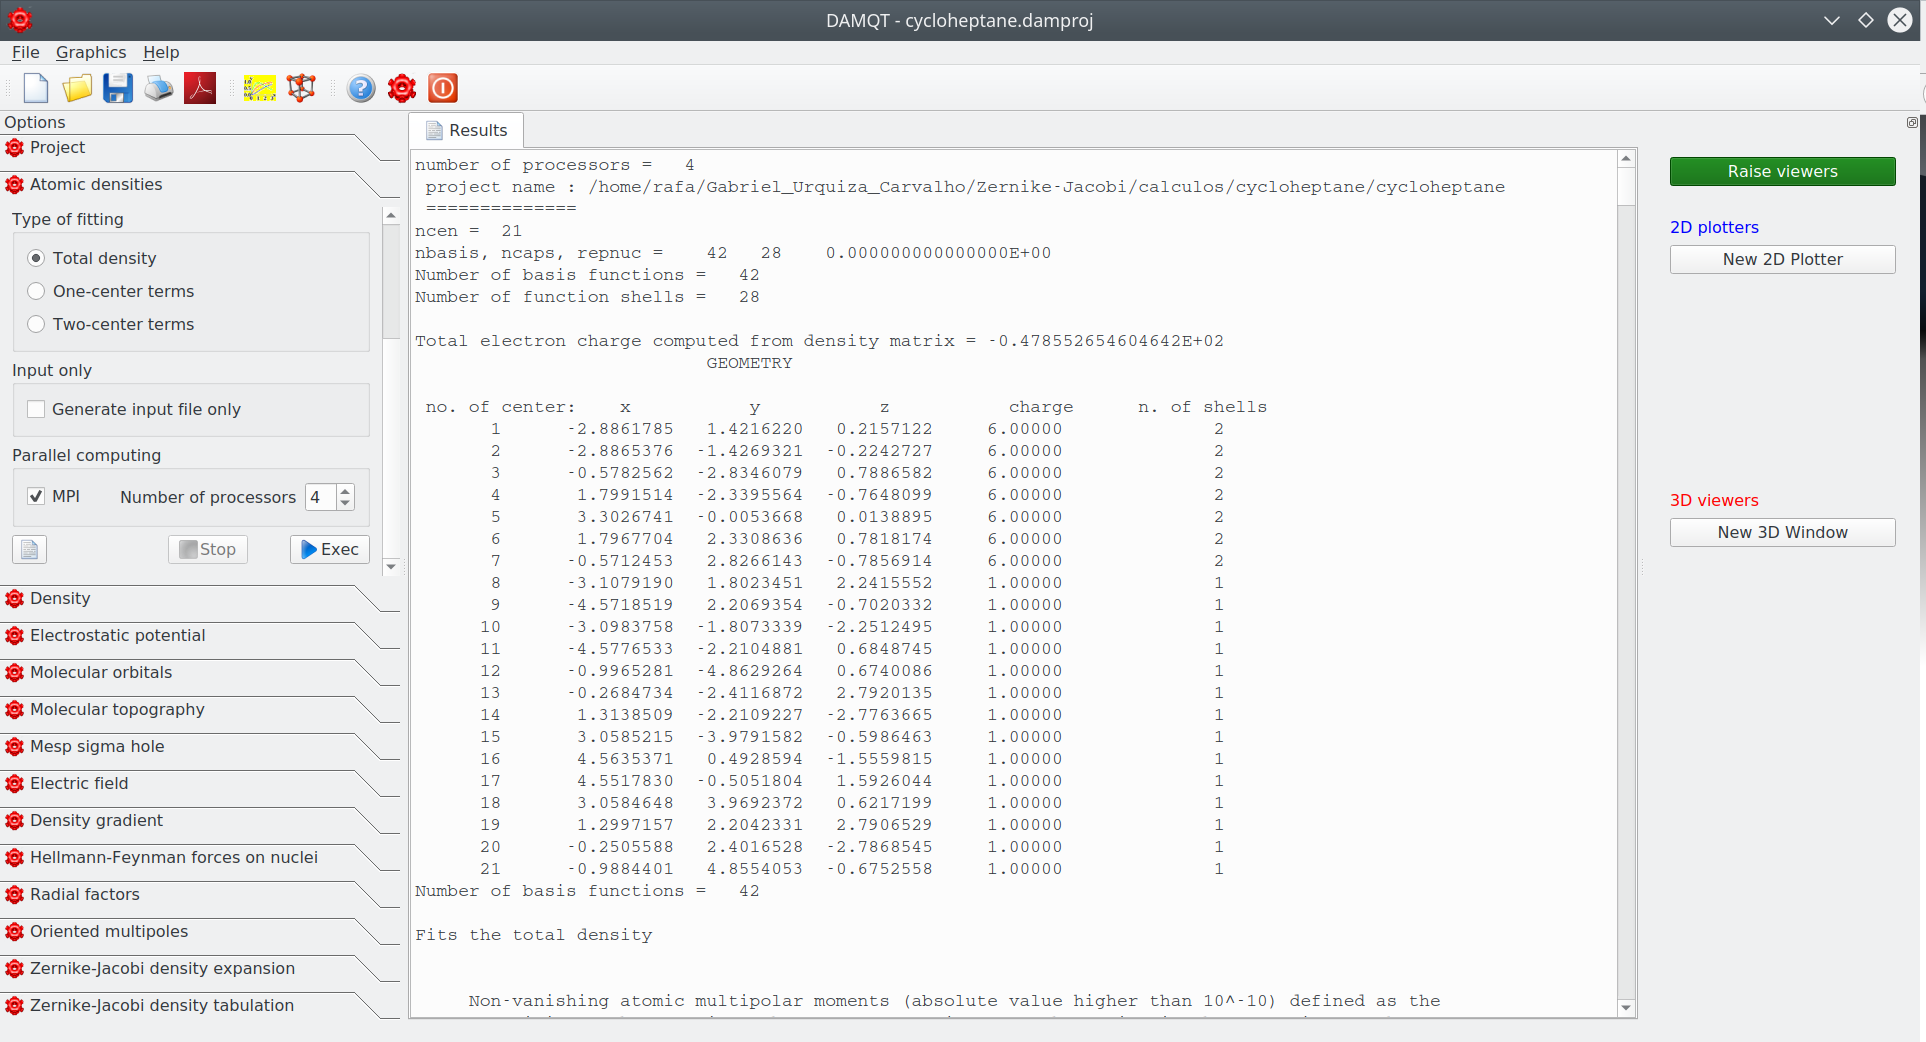
\includegraphics[width=0.5\linewidth]{damqt320_main_panel.png}
\end{center}
\caption{{DAMQT} main window \label{fig:2_1}}
\end{figure}

\vspace*{0cm}
\begin{figure}[H]
\begin{center}

\includegraphics[width=0.5\linewidth]{damqt320_toolbar.png}
\end{center}
\caption{{DAMQT} toolbar \label{fig:2_2}}
\end{figure}

The toolbar\index{toolbar} (fig. \ref{fig:2_2}) contains common options for this
program, namely:


\begin{description}
 \item[\bigtoolbN New file] Clears all options to start a new project
 \item[\bigtoolbA Open project] Opens an existing  project
 \item[\bigtoolbS Save project] Saves the current project
 \item[\bigtoolbP Print] Sends the content of the {\it Results} panel to the selected printer
 \item[\bigtoolbD Pdf file] Exports the content of the {\it Results} panel as a PDF file.
 \item[\bigtoolbE External program] Launches an external program
 \item[\bigtoolbC 2D viewer] Opens the  2D viewer
 \item[\bigtoolbV 3D viewer] Opens the  3D viewer
 \item[\bigtoolbH Help] Displays this manual.
 \item[\bigtoolbB About] Shows program information.
 \item[\bigtoolbQ Exit] Closes the program.
\end{description} 

The driving menu on the left side of the main window is used to access the different modules of DAMQT.
Its contents and functionality are described in this section.

Graphical tools can be launched from either the toolbar or the menu on the right
by clicking the {\it New 2D Plotter} or {\it New 3D Viewer} buttons.
When graphical tools are in use, entries for all currently open 2D and 3D viewers
will be displayed to facilitate navigation between them.

Each open viewer provides three buttons labeled:
\begin{itemize}
\item {\it Raise} $\rightarrow$ Brings the viewer to the foreground.
\item {\it Hide} $\rightarrow$ Toggles between hiding and showing the viewer.
\item {\it Delete} $\rightarrow$ Removes the viewer along with all its content.
\end{itemize}

Additionally, all open viewers can be raised to the foreground simultaneously
by clicking the {\it Raise all viewers} button at the top of the menu


\subsection{Project \label{sec:2.1}\index{project}}


Every project requires input files containing data from an LCAO calculation at any computational level.
At a minimum, one file is always required, with the extension \ggbs{}\index{ggbs@\textsl{ggbs} file} (for GTOs) or
\sgbs{}\index{sgbs@\textsl{sgbs} file} (for STO), which contains the geometry, nuclear charges, and basis set.

When DAM partition/expansion is needed, an additional file with the extension \den{}\index{den@\textsl{den} file}
must be provided. This file contains the elements of the density matrix (lower triangular part).

For storage efficiency, DAMQT also supports gzip\index{gzip} compressed \den{} files,
which are expected to have the extension \dengz{}.

Additionally, DAMQT can handle binary files containing sparse density matrices,
storing only the nonzero elements of the lower triangle in the format $i,j,\rho_{ij}$.
In this case, the expected file extension is {\it .densprsbin}.


% \vspace*{-5mm}
\begin{figure}[H]
\begin{center}
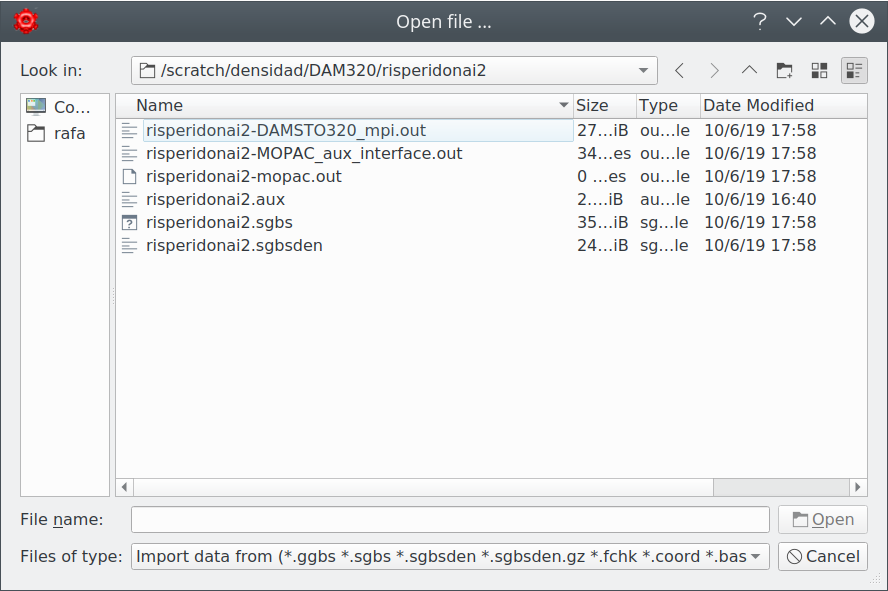
\includegraphics[width=.6\linewidth]{damqt_fig_2_1_1.png}
\end{center}
\caption{Import file navigator \label{fig:2_1_1}}
\end{figure}

Files \ggbs{ }, (\sgbs{ }), and \den{ }, \dengz{ }, or {\it .densprsbin}
can be loaded by entering their full name (including the path)
in the {\it Import data from} field.

Alternatively, the following file types can be supplied:
\begin{itemize}
\item GAUSSIAN\footnotemark\index{GAUSSIAN} {\it .fchk} files
\item MOLEKEL\index{MOLEKEL} {\it .mkl} files
\item TURBOMOLE\index{TURBOMOLE} basis set, coordinates, or molecular orbital files ({\it .basis}, {\it .coords}, {\it .mos})
\begin{quote}
\item These must be renamed to share a common name with the corresponding extensions.
\end{quote}
\item MOLPRO\index{MOLPRO} output files {\it .out}
\item \xml{ } files
\item NWCHEM\index{NWCHEM} output files {\it .nwcout}
\item MOPAC\index{MOPAC} {\it .aux} files
\item PSI4\index{MOPAC} {\it .psiauxden} files
\end{itemize}

For each of these formats, a built-in interface\index{interfaces} included in the package
will automatically generate the necessary \ggbs{ } and \den{ } files from the output files
of the corresponding software. See section \ref{sec:Interfaces} ({\it Interfaces}) of this manual for details.

Pressing \teclapuntos, a window will open, allowing navigation through the directory tree
(see fig. \ref{fig:2_1_1}) to select any of these files.


\vspace*{5mm}

\begin{minipage}{.35\linewidth}
\vspace*{-2mm}
\begin{figure}[H]
\vspace*{-3mm}
\begin{center}
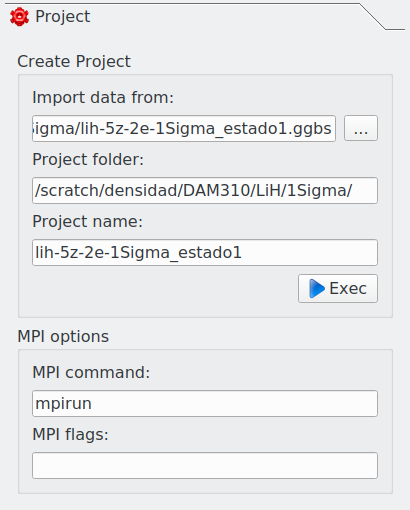
\includegraphics[width=.7\linewidth]{damqt320_project_menu.png}
\end{center}
\caption{Project \label{fig:2_1_2}}
\end{figure}
\end{minipage}
\hspace*{1cm}
\vspace*{5mm}
\begin{minipage}{.45\linewidth}
\begin{table}[H]
\begin{center}
\caption{\label{tab:2.1}Suitable file extensions for running interfaces}
\begin{tabular}{l|c}
interface & extensions \\
\hline
GAUSSIAN & *.fchk \\
MOLEKEL & *.mkl \\
MOLPRO & *.out, *.xml \\
MOPAC & *.aux \\
NWCHEM & *.nwcout \\
PSI4 & *.psiauxden \\
TURBOMOLE & *.basis, *.coords, *.mos \\
\hline
\end{tabular}
\end{center}
\end{table}
\end{minipage}

{\bf WARNING:} The current version of DAMQT only supports {\bf spherical functions}.
This is particularly important for Gaussian basis sets, which must be spherical\index{gaussians!spherical},
not Cartesian\index{gaussians!cartesian}.

For example, when performing molecular calculations with GAUSSIAN,
it may be necessary to include the {\it 5d,7f} options in the input file.

Alternatively, the \ggbs{ } and \den{ } files can be manually written
following the guidelines provided in Appendix \ref{A1}.
Additional interfaces for other standard packages may be implemented in future versions.

Project files will be stored in the directory specified in the {\it Project folder}
(see fig. \ref{fig:2_1_2}). By default, the application will assign the project name
based on the \ggbs{ } or \sgbs{ } file name,
but this can be modified by entering a different name in the {\it Project name} field.

All files generated within the project will share the project name,
unless explicitly specified otherwise in the module menus.

To run an interface, simply select an appropriate file type
from the extensions listed in Table \ref{tab:2.1}.
 
\footnotetext{www.gaussian.com}

\begin{center}
\begin{minipage}{.25\linewidth}
\begin{figure}[H]
\begin{center}
\vspace*{-2mm}
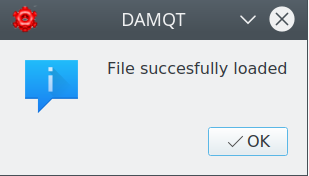
\includegraphics[width=.6\linewidth]{damqt320_info_load.png}
\end{center}
\caption{Project upload \label{fig:2_1_3}}
\end{figure}
\end{minipage}
\begin{minipage}{.25\linewidth}
\begin{figure}[H]
\begin{center}
\vspace*{-2mm}
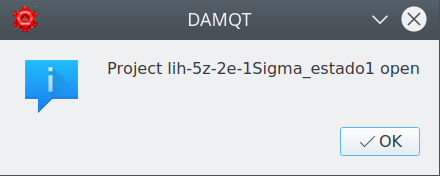
\includegraphics[width=.87\linewidth]{damqt320_info_open.png}
\end{center}
\caption{Project opening\label{fig:2_1_4}}
\end{figure}
\end{minipage}
\end{center}

If an existing \ggbs{ } or \sgbs{ } file is selected, a message
similar to the one shown in fig. \ref{fig:2_1_3} will appear, confirming or denying the upload.
This will be followed by another message confirming the project opening (fig. \ref{fig:2_1_4}).

Once the required files are located, the \exec key must be pressed to:
\begin{itemize}
\item Build the \ggbs{ } (\sgbs{ }) and \den{ } files using the interfaces to standard packages, or
\item Load them if they already exist.
\end{itemize}

At the same time, a \damproj{ } file will be created,
containing the default values required to run the remaining modules.
This process must be completed at least once for each project.

To load an existing project, either:
\begin{itemize}
\item Click the \toolbA icon in the toolbar, or
\item Select {\it File $\rightarrow$ Open project} from the top menu,
navigate to the desired project, and select one of the displayed files.
\end{itemize}

Recent projects can also be accessed directly from the {\it File} menu.

For systems with {\it mpi}, two additional fields will appear
to specify the command for executing {\it mpi} programs
and the appropriate {\it mpi} flags (see fig. \ref{fig:2_1_2}).
DAMQT automatically checks whether {\it mpirun} or {\it mpiexec}
is installed on the system (in that order).
If either is found, it is automatically assigned to the {\it MPI command} field.

\subsection{Atomic densities \label{sec:2.2}\index{atomic densities}}

\begin{center}
\begin{minipage}{.59\linewidth}

The tab in the driving menu labeled {\it Atomic densities} invokes either the DAMSTO or DAMGTO programs,
which compute the atomic expansion of the density—the cornerstone of the DAMQT partition/expansion,
as illustrated in fig. \ref{fig:1}.

One of these programs must be executed at least once per project,
except for molecular orbital plotting or Zernike-Canterakis/Jacobi expansions.
The package also includes parallel computing versions of these programs using {\it mpi}\index{parallel computing}.

To accommodate installations where parallel programs can only be batch processed,
or if the user prefers to run density partitioning and fitting programs
outside the DAMQT environment, an option is available to generate only the input file.

The exponents and coefficients for the piecewise representation of the radial factors
are stored in a file with the extension \damqt{ }, which will be read by the remaining modules.

Figure \ref{fig:2_2_1} displays the menu that appears when this tab is selected.

\end{minipage}
\begin{minipage}{.4\linewidth}

\begin{figure}[H]
\begin{center}
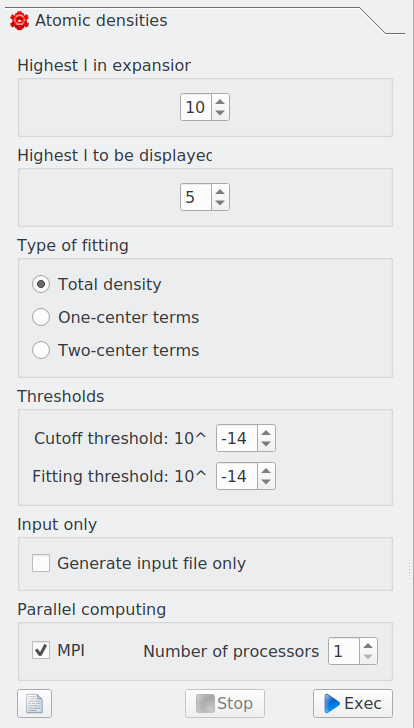
\includegraphics[width=.55\linewidth]{damqt320_atomic_densities.png}
\end{center}
\caption{Atomic densities menu \label{fig:2_2_1}}
\end{figure}

\end{minipage}
\end{center}

The following options can be set\index{atomic densities!options}:

\begingroup
\renewcommand{\labelitemi}{$-$}
\begin{itemize}
\item {\it Highest l in expansion}: Defines the order of the multipole expansion.
The maximum allowed value is 25 (default: 10).
Expansions with the default order yield an absolute error in the atomic contributions
to the density estimated to be less than $10^{-5}$ a.u., except at points near the nuclei,
where around five significant figures are expected to be accurate.

\item {\it Highest l to be displayed}: Determines the highest multipole order ($l$)
of atomic and molecular components that will be displayed and printed in the output file.
It must be less than or equal to the highest $l$ in the expansion (default: 5).

\item {\it Type of fit\index{atomic densities!type of fit}}: The usual choice is to fit the total density (default),
but representations of one-center or two-center contributions to density
in the LCAO framework can also be performed.
For calculations using the ZDO approximation (MOPAC), the {\it only one-center} option
is automatically selected to maintain consistency.

\item {\it Thresholds\index{atomic densities!thresholds}}:
Defines the thresholds for:
\vspace*{-5mm}
\begin{quote}
\item Neglecting radial factors ({\it Cutoff})
\item Truncating radial factor expansions in Chebyshev polynomials ({\it Fitting})
\end{quote}

\item {\it Input only\index{atomic densities!input only}}:
Generates the input file with the selected options,
but does not perform partitioning or fitting.

\item {\it Parallel computing\index{atomic densities!parallel computing}}:
For systems with {\it mpi} installed, parallel versions of DAMSTO and DAMGTO can be executed.
The number of processors can be selected but must be less than or equal to the number of atoms in the system.
This option will remain hidden on systems where {\it mpi} is unavailable or on MS-Windows.
{\bf Warning:} This option is not suitable for running MPI batch processes.
\end{itemize}
\endgroup

To compute the expansion, press the \exec key.
In addition to the \damqt{ } file, another file ending in \dmqtv{ }
will be created, containing auxiliary integrals for electrostatic potential computations.

Additionally, information will be displayed in the standard output (see fig. \ref{fig:2_2_2}), including:

\begin{itemize}
\item Project name
\item Geometry
\item Basis set size
\item Total electron charge retrieved from the density (without partitioning)
\item Nonzero atomic multipole moments up to the highest order chosen for printing
\item Molecular charge and multipoles computed from partitioning
\end{itemize}

Note that, in general, the multipole order used for printing is lower
than that used for density fitting and computations—
meaning only a subset of the computed and stored multipoles will be printed.

This information is also stored in a file named:
{\it projectname}-DAMGTO320.out (for GTO densities),
where {\it projectname} corresponds to the current project name.

For STO densities, DAMGTO will be replaced by DAMSTO.

\vspace*{0.3cm}

% \vspace*{-1.cm}
\begin{center}
\begin{tabular}{cc}
\begin{minipage}{.48\linewidth}
\begin{figure}[H]
\begin{center}
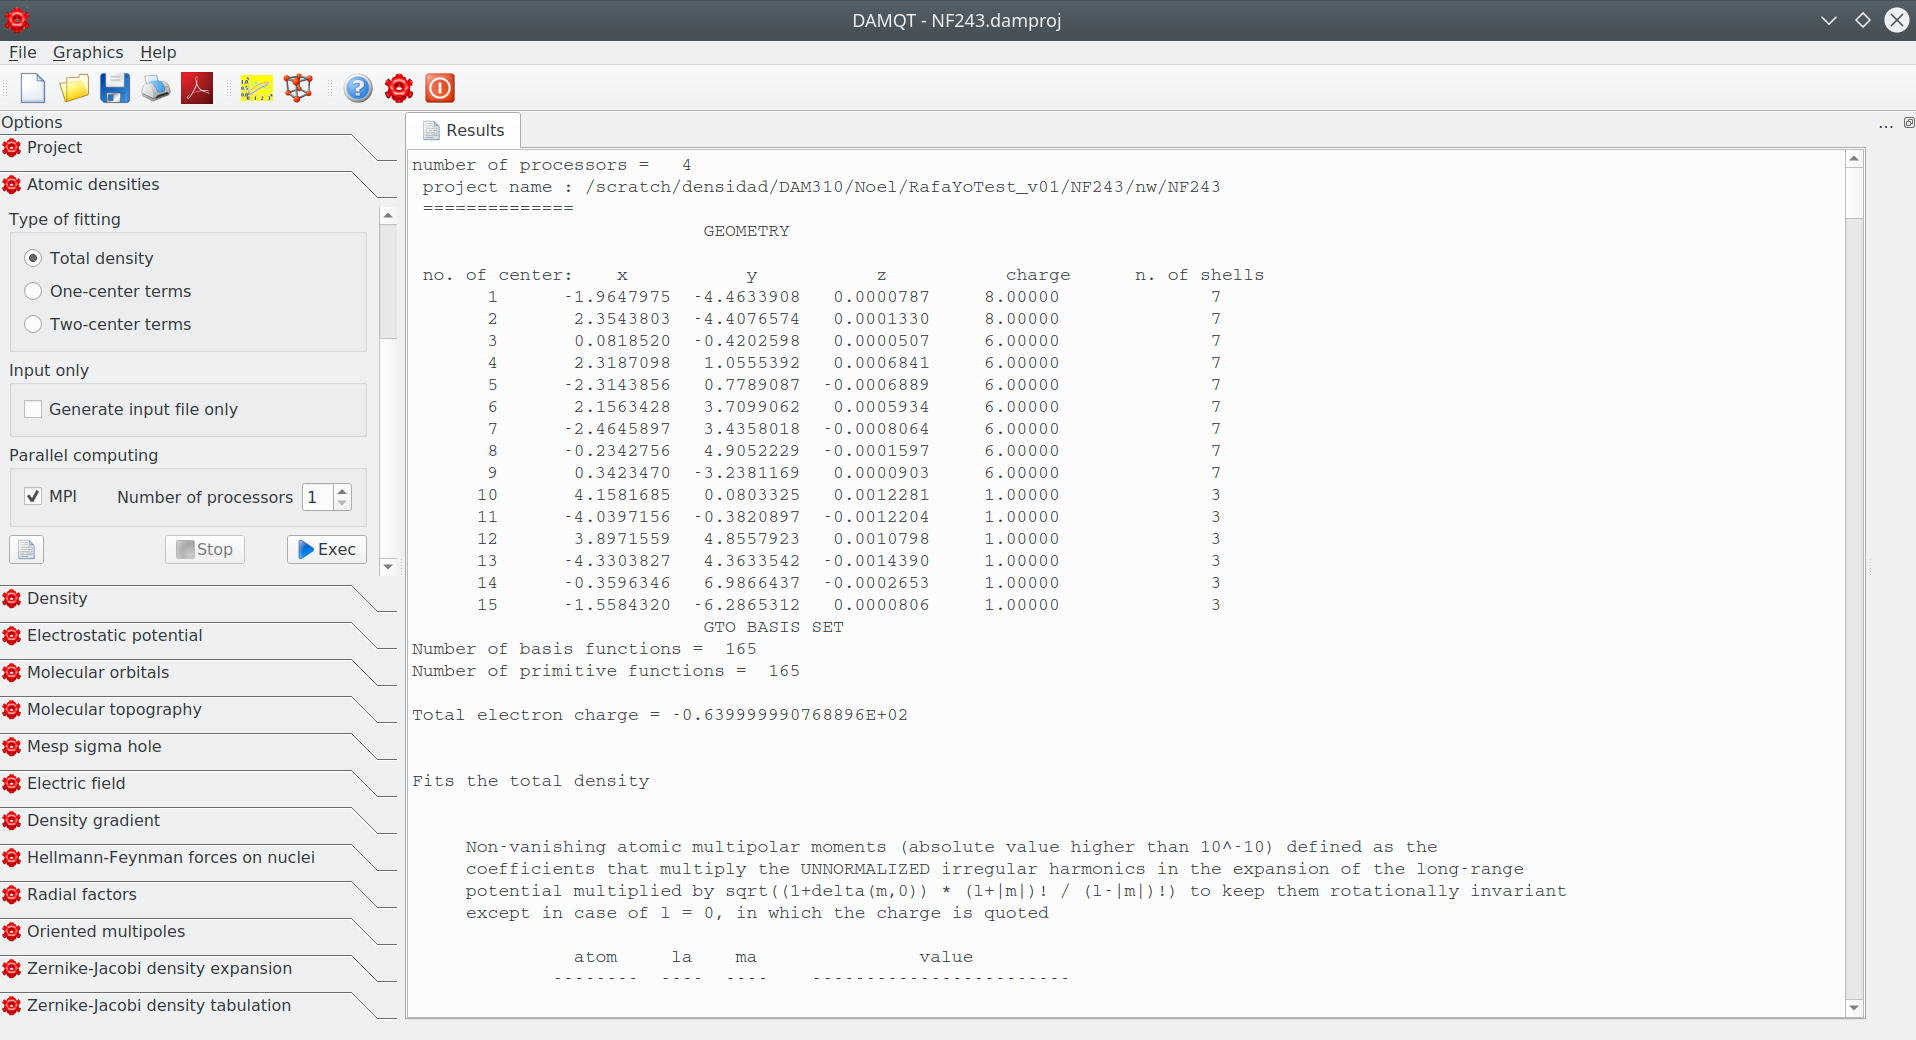
\includegraphics[width=.9\linewidth]{damqt320_standard_output.png}
\end{center}
\caption{{Standard output} \label{fig:2_2_2}}
\end{figure}
\end{minipage}
&
\begin{minipage}{.48\linewidth}
\begin{figure}[H]
\begin{center}
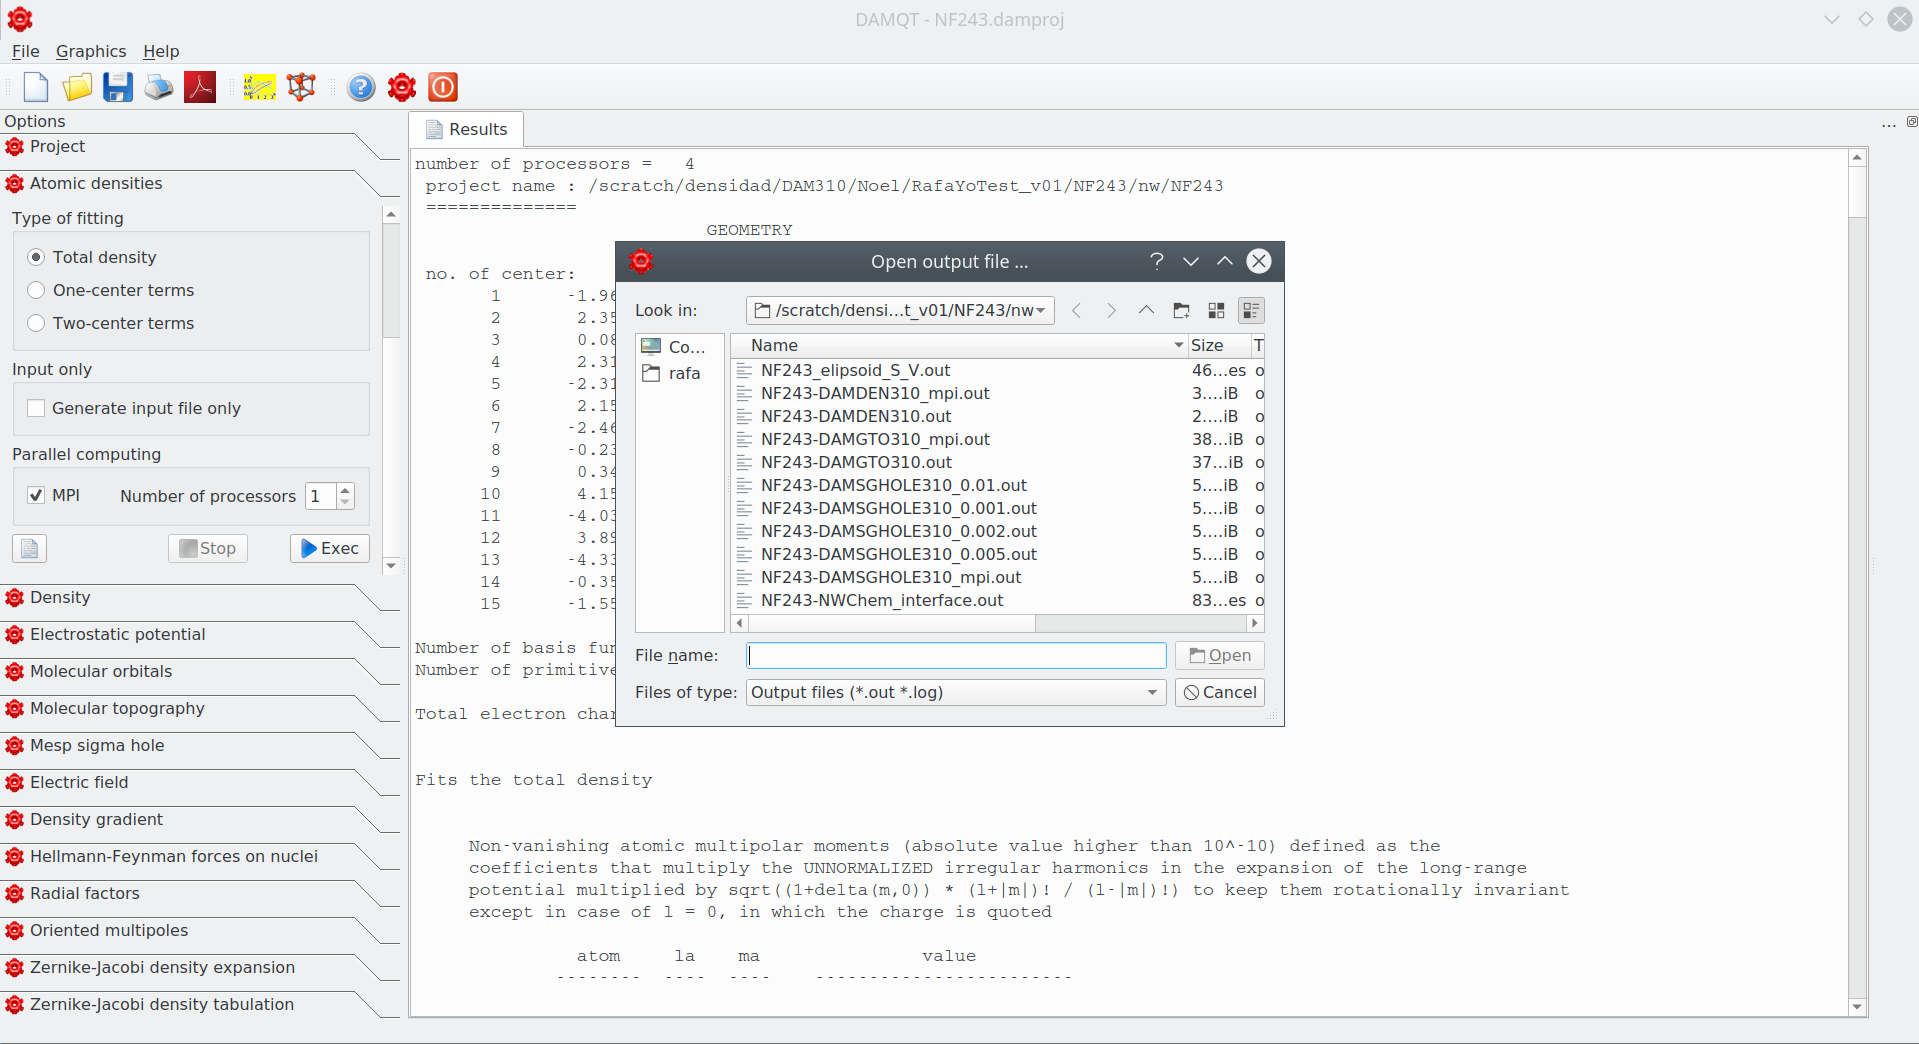
\includegraphics[width=.9\linewidth]{damqt320_output_files_menu.png}
\end{center}
\caption{{Standard output files menu}\label{fig:2_2_3}}
\end{figure}
\end{minipage}
\end{tabular}
\end{center}


% \end{minipage} &

\vspace*{5mm}

\begin{tabular}{lr}
\hspace*{-3mm}
\begin{minipage}{.6\linewidth}

Another file with the extension {\it .mltmod}, containing the moduli of the atomic multipole moments\index{multipole moments},
is also generated.

The multipole moments are defined as the coefficients that multiply the
{\it unnormalized} irregular spherical harmonics in the expansion of the long-range potential.
Since the moduli of spherical harmonics depend on the value of $|m|$,
the values stored in the {\it .mltmod} file correspond to the multipole moments $Q_{lm}$,
each multiplied by:
$$
(1 + \delta_{m0}) \; \sqrt{(l+|m|)!/(l-|m|)}!
$$
to preserve rotational invariance.

The \stopkeya key allows stopping the process.
The \listados key displays a list of all currently available \out{ } files (see fig. \ref{fig:2_2_3}).
The contents of these files can be viewed in the main panel.

\subsection{Density \label{sec:2.3}\index{density}}

The {\it Density} tab provides access to the module for density tabulation
and grid generation for 2D contour plots and 3D images (see fig. \ref{fig:2_3_1}).

This module can process density data either from:

\begin{itemize}
\item Any standard package for molecular calculations ({\it Original density})—i.e., expressed in terms of the basis set, or
\item The atomic expansion of the density generated by DAM ({\it Fitted density}\index{density!options}) (default).
\end{itemize}

When using {\it Original density}\index{density!original}, tabulation
and grid generation can only be performed for the full molecular density.

The {\it Fitted density}\index{density!fitted density} option (default) provides additional capabilities:
 
\end{minipage} &
\begin{minipage}{.4\linewidth}
% \vspace*{-5mm}
\begin{figure}[H]
% \vspace*{-5mm}
\begin{center}
\includegraphics[width=.48\linewidth]{damqt320_density_1.png} \\
\vspace*{-1mm}
\includegraphics[width=.48\linewidth]{damqt320_density_2.png} \\
\end{center}
\caption{Density menu \label{fig:2_3_1}}
\end{figure} 
\end{minipage}
\end{tabular}

\newpage
Three density modes are available:

\begin{itemize}
\item {\it Full electron density}\index{density!full electron density}
\vspace*{-5mm}
\begin{quote}
\item Uses an expansion from $l = 0$ up to a user-defined $l_{max}$
(which must be $\le$ the highest available).
\end{quote}
\item {\it Density deformations}\index{density!density deformations}
\vspace*{-5mm}
\begin{quote}
\item Uses an expansion from $l = 1$, effectively removing atomic spherical terms.
\end{quote}
\item {\it Contributions to density}\index{density!contributions to density}
\vspace*{-5mm}
\begin{quote}
\item Allows selecting a specific range of $l$ values.
\end{quote}
\end{itemize}

For each case, the multipole terms included in the atomic expansions
can be adjusted using the spinboxes under {\it Atomic terms}, following the corresponding restrictions.

Results obtained with the {\it Full electron density} mode will be similar
to those of the {\it Original density} option, but replacing the original density
with its atomic multipole expansion up to the selected order.

When {\it Highest l} is set to 5 or greater,
the resulting plots will be indistinguishable from those generated with the {\it Original density} option.

\vspace*{3mm}
{\bf Visualizing Density Deformations}
\vspace*{3mm}

Selecting {\it Density deformations} allows visualization of the bond skeleton\index{bond skeleton} of molecules,
along with various structural patterns that correlate with fundamental concepts in empirical structural chemistry,
such as:

\begin{itemize}
\item Lone pairs\index{lone pairs}
\item Single, double, and triple bonds
\item Electron delocalization\index{electron delocalization}
\item And more
\end{itemize}

To achieve smooth 3D surfaces in moderate-sized systems, it is recommended
to enable the {\it gradient}\index{density!gradient} option.
This ensures that grid gradient components are computed analytically,
which approximately doubles computation time compared to density calculations alone.

For large systems, details on obtaining smooth surfaces
can be found in section \ref{sec:4.13.10}\index{smooth surfaces}.

Furthermore, using the atomic expansion, it is possible to obtain atomic contributions to density
or atomic deformations\index{atom deformations} for individual atoms or groups of atoms (functional groups)\index{functional groups}.

Enabling the {\it Atomic fragments} checkbox displays a table
where users can select atoms whose densities or deformations
should be individually tabulated (see fig. \ref{fig:2_3_2}).

Selecting the {\it Functional group} checkbox allows the density or deformations
to be tabulated for the selected atoms collectively.
The indices of the selected centers can be entered in the input box,
either separated by commas or as ranges, using a hyphen to separate the start and end indices.

The {\it Grid}\index{density!grid} options determine whether a grid for 2D plots
or a 3D density/deformation image will be generated.

If the {\it Generate grid} box is checked (default) and the 2D grid option is selected,
a panel similar to fig. \ref{fig:2_3_3} will appear for tabulation settings.

2D grids\index{2D grid!grid definition} are defined using two variables, $u$ and $v$,
whose tabulation ranges are specified in the input fields labeled {\it Lowest} and {\it Highest}.

The {\it Plane} option performs tabulation on a plane.
Buttons are provided to select predefined planes: $XY$, $XZ$, and $YZ$,
or to define an arbitrary plane.

When the {\it Other} button is checked, additional input fields appear,
allowing users to specify the parameters for the arbitrary plane.

\vspace*{1mm}
\begin{tabular}{lr}
\hspace*{-3mm}
\begin{minipage}{.6\linewidth}
Enabling the {\it Parametric surface} option allows tabulation for a set of spatial coordinates
$x$, $y$, and $z$, computed as functions of $u$ and $v$:
$$
x(u,v), y(u,v), z(u,v)
$$
Standard arithmetic operators ($+$, $-$, $*$, $/$, $\hat{\ }$)
as well as mathematical functions ($\sin$, $\cos$, $\tan$, $\log$, $\ln$, $\mbox{abs}$,
$\exp$, $\mbox{\\sqrt{ }}$) can be used to define $x$, $y$, and $z$,
providing high flexibility in choosing 2D surfaces.

Three predefined resolution levels are available:

\begin{itemize}
\item {\it Low} (129x129)
\item {\it Medium} (257x257)
\item {\it High} (513x513)
\end{itemize}

Alternatively, custom resolution can be set by pressing the {\it Custom} button,
which enables spin-boxes to adjust the resolution in both dimensions.
The values entered in these boxes define the number of voxels in each direction
(i.e., the number of points minus one).

Tabulated 2D grid values are stored in a file named according to the label
set in the {\it Output file prefix} option, with the extension \cnt.
{\bf Warning:} Parallel computing is not supported for 2D grid tabulation.

\vspace*{3mm}
{\bf 3D Grid Tabulation}
\vspace*{3mm}

If the 3D grid\index{3D grid!grid definition} option is selected (see fig. \ref{fig:19}),
the grid will form a box with dimensions defined by the $x$, $y$,
and $z$ coordinates, specified in the input fields labeled {\it Lowest} and {\it Highest}.

Three predefined resolution levels are available:

\begin{itemize}
\item {\it Low} (65x65x65)
\item {\it Medium} (129x129)
\item {\it High} (257x257)
\end{itemize}

A custom resolution option is also available.

Tabulated 3D grid values are stored in files named according to the label
set in the {\it Output file prefix} option, with the extension \plt.
These files are compatible with 3D plotting software such as gOpenMol\footnotemark\index{gOpenMol}.

\end{minipage}
&
\begin{minipage}{.4\linewidth}

\vspace*{-5mm}
\begin{figure}[H]
\vspace*{-0.5cm}
\begin{center}
\includegraphics[width=.55\linewidth]{damqt_fig_2_3_2.png}
\end{center}
\caption{Single atom densities \label{fig:2_3_2}}
\end{figure}

% \vspace*{-5mm}
\begin{figure}[H]
\vspace*{-5mm}
\begin{center}
\includegraphics[width=.5\linewidth]{damqt_fig_2_3_3.png}
\end{center}
\caption{2D Grid settings\label{fig:2_3_3}}
\end{figure}

% \vspace*{-5mm}
\begin{figure}[H]
\vspace*{-5mm}
\begin{center}
\includegraphics[width=.5\linewidth]{damqt_fig_2_2_7.png}
\end{center}
\caption{3D Grid settings\label{fig:19}}
\end{figure}
\end{minipage}
\end{tabular}
\vspace*{1mm}


For systems with {\it mpi} installed, parallel computing can be enabled,
similar to the {\it Atomic densities} module.

To distinguish the different grid files generated (including those for electrostatic potentials),
the following naming conventions apply:

\begin{itemize}
\item {\it \$fname-d.cnt}: 2D grid tabulation file for the full molecular density or deformations.
\item {\it \$fname-d-d?.cnt}: 2D grid tabulation files containing first derivatives of the density or deformations ({\it ?} = $x, y, z$).
\item {\it \$fname-d-d??.cnt}: 2D grid tabulation files containing second derivatives ({\it ??} = $xx, xy, ... zz$).
\item {\it \$fname-d-lplc.cnt}: 2D grid tabulation files containing the Laplacian of the atomic density or deformation.
\item {\it \$fname-d.plt}: 3D grid tabulation file for the full molecular density or selected density contributions.
\item {\it \$fname-deform-d.plt}: 3D grid tabulation file for molecular density deformations.
\item {\it \$fname-cxx-d.plt}: 3D grid tabulation file for the atomic density of the {\it xx$^{th}$} center,
according to the ordering in the geometry definition.
\item {\it \$fname-deform-cxx-d.plt}: 3D grid tabulation file for the atomic density deformation
of the {\it xx$^{th}$} center, according to the ordering in the geometry definition.
\item {\it \$fname-frg-d.plt}: 3D grid tabulation file for the density of a selected group of atoms (functional group).
\item {\it \$fname-frg-deform-d.plt}: 3D grid tabulation file for the density deformation of a selected group of atoms.
\item {\it \$fname-*-d-d?.pltd}: 3D grid tabulation files containing first derivatives of the density or deformations ({\it ?} = $x, y, z$).
\item {\it \$fname-*-d-d??.pltd}: 3D grid tabulation files containing second derivatives of the density or deformations ({\it ??} = $xx, xy, ... zz$).
\item {\it \$fname-*-d-lplc.plt}: 3D grid tabulation files containing the Laplacian of the atomic density or deformations.
\end{itemize}
%
Here, {\it \$fname} represents the root name of the file.

\vspace*{3mm}
{\bf Molecular Density Tabulation at Selected Points}
\vspace*{3mm}

In addition to grid generation, molecular density or its deformations
can be tabulated at specific points.

To enable this, check the {\it Tabulation points} box and specify the desired points in the table.
The tabulated values will be:

\begin{itemize}
\item Printed in the corresponding \out{ } file
\item Displayed in the main panel
\end{itemize}

Options for input file generation and parallel computation
are also available, similar to those in the density partition and fit module.

\subsection{Electrostatic potential \label{sec:2.4}\index{electrostatic
potential}}

The {\it Electrostatic potential} tab invokes the module for electrostatic potential tabulation
and grid generation for 3D images (see fig. \ref{fig:2_4_1}).

The electrostatic potential is computed using the density representation.
The number of terms included in the expansion is controlled via the spinbox labeled {\it Highest l in expansion}.

\vspace*{3mm}
{\bf Long-Range Computation}
\vspace*{3mm}

To compute the electrostatic potential using point atomic multipoles,
enable the {\it Long-range only}\index{electrostatic potential!long-range} checkbox.

If this option is disabled, a long-range threshold is applied:

\begin{itemize}
\item The long-range expansion will be used only if the estimated contribution of the short-range terms
is smaller than the threshold.
\item Otherwise, the radial factors (which depend on $r$) will be used instead.
\end{itemize}

\begin{tabular}{lr}
\hspace*{-3mm}
\begin{minipage}{.6\linewidth}


\vspace*{3mm}
{\bf Grid Definitions and Smooth Surface Options}
\vspace*{3mm}

For 2D and 3D grid definitions, the same considerations as in the {\it Density} module apply,
including the resolution options.

To generate smooth 3D surfaces in moderate-sized systems,
enable the {\it gradient}\index{electrostatic potential!gradient} option.
This ensures that grid gradient components are computed analytically,
which approximately doubles computation time compared to electrostatic potential calculations alone.

For large systems, details on obtaining smooth surfaces can be found in section \ref{sec:4.13.10}\index{smooth surfaces}.

For systems with {\it mpi} installed, parallel computing can be enabled,
similar to the {\it Atomic densities} module.

\vspace*{3mm}
{\bf File Naming Conventions}
\vspace*{3mm}

File naming conventions for electrostatic potential grid files\index{electrostatic potential!grid}
follow the same structure as those for density grid files:

\begin{itemize}
\item {\it \$fname-p.plt} $\rightarrow$ 3D grid tabulation file for the electrostatic potential.
\item {\it \$fname-p-d?.pltd} $\rightarrow$ Files with first derivatives of the potential ({\it ?} = $x, y, z$).
\item And so forth…
\end{itemize}

The root name {\it \$fname} can be defined in the {\it Output file prefix} field.
These files are compatible with gOpenMol.

Options for input file generation and parallel computation are also available.

\end{minipage}
&
\begin{minipage}{.4\linewidth}

\begin{figure}[H]
\begin{center}
\vspace*{-5mm}
\includegraphics[width=.65\linewidth]{damqt_fig_2_4_1.png}
\end{center}
\caption{Electrostatic potential \label{fig:2_4_1}}
\end{figure}
\end{minipage}
\end{tabular}
\vspace*{0.1mm}
\footnotetext{www.csc.fi/gopenmol/}


\subsection{Molecular orbitals \label{sec:2.5}\index{molecular orbitals}}

The {\it Molecular orbitals}\index{molecular orbitals} tab generates 2D and 3D grids
for plotting molecular orbitals (see fig. \ref{fig:2_5_1}).

For options and grid definitions, the same considerations as in
sections \ref{sec:2.3} and \ref{sec:2.4} apply.

The indices of the molecular orbitals to be plotted should be entered in the {\it Molecular orbitals} field,
separated by commas. To specify a range of indices, use hyphens as separators.

Molecular orbitals are sorted in ascending energy.

For UHF calculations with MOLPRO, different orbital sets may be generated
depending on the interface used. See section \ref{sec:5.2} for details.


\subsection{Molecular topography \label{sec:2.6}\index{molecular topography}}

The {\it Molecular topography}\index{molecular topography} tab is designed for:

\begin{itemize}
\item Mapping critical points (CPs)\index{molecular topography!critical points}
\item Determining the molecular graph\index{molecular topography!molecular graph}
\item Computing atomic basin borders\index{molecular topography!atomic basin}
\end{itemize}

These calculations can be performed for both electron density and electrostatic potential (see fig. \ref{fig:2_6_1}).

Mapping all critical points is the first essential step required
before proceeding with molecular graph determination and atomic basin calculations.

\vspace*{10mm}

\begin{tabular}{lcr}
\begin{minipage}{.53\linewidth}
\begin{figure}[H]
\begin{center}
\vspace*{-6.4mm}
\includegraphics[width=.45\linewidth]{damqt_fig_2_5_1.png}
\end{center}
\caption{{Molecular orbitals}\label{fig:2_5_1}}
\end{figure}
\end{minipage}
&
\begin{minipage}{.47\linewidth}
\begin{figure}[H]
\begin{center}
\vspace*{-8mm}
\includegraphics[width=.52\linewidth]{damqt_fig_2_6_1a.png}
\includegraphics[width=.52\linewidth]{damqt_fig_2_6_1b.png}
\end{center}
\caption{Molecular topography \label{fig:2_6_1}}
\end{figure}
\end{minipage}
\end{tabular}

\vspace*{5mm}

The values of density (MED) and electrostatic potential (MESP),
along with their gradient and second derivatives,
are computed while identifying critical points (CPs)
using the DAM partition/expansion method.

The number of terms included in the expansion for field value calculations
can be set using the spinbox labeled {\it Highest l in expansion}.

\vspace*{3mm}
{\bf Guess Point Generation for CP Search}
\vspace*{3mm}

The initial guess points for locating critical points
are determined internally. However, for the electrostatic potential,
where CPs can be located far from the molecular skeleton,
the guess point generation requires gradient evaluation on a grid.

The grid size and step size can be adjusted
under the {\it Guess points} option by specifying:

\begin{itemize}
\item {\it Box size} (in atomic units)
\item {\it Step size} (in atomic units)
\end{itemize}

If necessary, users can manually add additional guess points
by selecting the {\it Add guess points for CPs} option.
These points can be provided via:

\begin{itemize}
\item A pop-up table, or
\item An external text file, where each row contains the $(x,y,z)$ coordinates of a point.
\end{itemize}

\vspace*{3mm}
{\bf Optimization of Guess Points}
\vspace*{3mm}

The guess points are optimized to critical points using
the L-BFGS subroutine, an iterative method for solving unconstrained nonlinear optimization problems.

The search for a critical point is performed within
a cubic region surrounding the initial guess point.

A cube with a side length of $0.5-1.0$ a.u.
is recommended for this purpose.

The cube size can be controlled using the
{\it Box margins size} option, which appears
when the {\it map critical points} option is selected.

A convergence threshold is required to determine
when the program has successfully located a critical point.
Recommended values are:

\begin{itemize}
\item $4 \cdot 10^{-16}$ for electron density
\item $4 \cdot 10^{-12}$ for electrostatic potential
\end{itemize}

\vspace*{3mm}
{\bf Molecular Graph Calculation}
\vspace*{3mm}

The molecular graph for MED and MESP-based topography
is computed using the {\it Gradient path}\index{molecular topography!gradient path} option.

This requires the presence of a critical point (CP) file.
If a CP file is missing, the program will automatically
perform critical point mapping before proceeding.

For gradient paths that extend to asymptotic regions,
a large bounding box with a recommended side length of 5.0 a.u. should be used.

\vspace*{3mm}
{\bf Atomic Basin Calculation}
\vspace*{3mm}

Atomic basins\index{topography!atomic basins}
for both MED and MESP are calculated under the {\it Atomic basin} option.

This computation requires:

\begin{itemize}
\item A critical point (CP) file
\item The molecular graph determination
\end{itemize}

Selecting {\it compute basin} will automatically enable the {\it Gradient path} option.

To refine the appearance of atomic basins,
the {\it Extra connections} checkbox can be selected,
and an appropriate {\it Connection threshold} value can be specified.
A higher threshold value results in more connecting lines appearing in the basin visualization.

\vspace*{3mm}
{\bf File Naming Conventions}
\vspace*{3mm}

The output files follow a structured naming convention:

\begin{itemize}
\item Critical Point Files:
\vspace*{-5mm}
\begin{quote}
\item {\it \$fname-cps-d.xyz} $\rightarrow$ Stores MED CPs
\item {\it \$fname-cps-v.xyz} $\rightarrow$ Stores MESP CPs
\item {\it \$fname-cps-d.eigv} $\rightarrow$ Contains eigenvector data for MED CPs
\item {\it \$fname-cps-v.eigv} $\rightarrow$ Contains eigenvector data for MESP CPs
\end{quote}

\item Molecular Graph Files:
\vspace*{-5mm}
\begin{quote}
\item {\it \$fname-d.gpdat} $\rightarrow$ Contains MED molecular graph data
\item {\it \$fname-v.gpdat} $\rightarrow$ Contains MESP molecular graph data
\end{quote}

\item Atomic Basin Files:
\vspace*{-5mm}
\begin{quote}
\item {\it \$fname-d.basins} $\rightarrow$ Stores MED atomic basin data
\item {\it \$fname-v.basins} $\rightarrow$ Stores MESP atomic basin data
\end{quote}
\end{itemize}

Options for input file generation and parallel computation
are also available.


\vspace*{5mm}
\begin{tabular}{lr}
\hspace*{-3mm}
\begin{minipage}{.6\linewidth}


\subsection{MESP sigma hole \label{sec:2.7}\index{MESP sigma hole}}

The {\it MESP sigma hole} tab provides access to the module for computing
the molecular electrostatic potential (MESP) on an isosurface
of density (MED) (see fig. \ref{fig:2_7}).

The MESP values at the vertices of the triangular mesh
decomposing the MED isosurface are stored in a file
with the extension $.sgh$.

\vspace*{3mm}
{\bf Local Extrema Search and Thresholding}
\vspace*{3mm}

In addition, local maxima and minima of MESP are identified,
provided they are higher (maxima) or lower (minima)
than a specified threshold.

The threshold is defined as a fraction
of the absolute extrema values and is set in the {\it Threshold for local extrema} field.
The default value is 0.70 (i.e., 70% of the absolute extrema values).

Due to numerical accuracy limitations in the mesh,
several maxima or minima may appear as distinct extrema
within the same region.

To mitigate this issue, a separation threshold
between extrema belonging to different regions
can be specified in the {\it Extrema separation} field.

\begin{itemize}
\item Extrema of the same type (i.e., maxima or minima)
that are separated by a distance smaller than this threshold
are considered part of the same extremum region.
\item In such cases, only the highest maximum (or lowest minimum)
is retained for the given region.
\end{itemize}

\vspace*{3mm}
{\bf MESP Histogram}
\vspace*{3mm}

A histogram\index{MESP sigma hole!histogram}
of MESP values on the isosurface is also generated.

This histogram represents a plot of surface area (in bohr$^2$) vs MESP values
and serves as a comparative tool for analyzing sigma holes
of different molecules.

\end{minipage}
&
\begin{minipage}{.4\linewidth}
\begin{figure}[H]
\begin{center}
\vspace*{-0.5mm}
\includegraphics[width=.8\linewidth]{damqt320_mesp_sg_hole.png}
\end{center}
\caption{{MESP sigma hole}\label{fig:2_7}}
\end{figure}
\end{minipage}
\end{tabular}

\vspace*{0.4mm}

To compute the sigma hole, the MED must first be tabulated on a 3D grid (see sec. \ref{sec:2.3}),
and the corresponding $.plt$ file must be selected in the {\it Import density grid from} field.

The MED value for the isosurface can be specified in the {\it Density value} field.


\vspace*{3mm}
{\bf Threshold Settings}
\vspace*{3mm}

Three thresholds can be set in their respective fields:

\begin{itemize}
\item Geometry threshold: Two points are considered the same if they are separated
by a distance smaller than this threshold.
\item MESP long-range threshold: Short-range contributions are ignored
when they fall below this value.
\item Local extrema threshold: Defines the minimum prominence required
for an extremum to be considered significant.
\end{itemize}

\vspace*{3mm}
{\bf Computation Method: DAM Expansion vs. Exact Potential}
\vspace*{3mm}

The MESP can be computed using two different methods:

\begin{enumerate}
\item DAM expansion of density (recommended)
\item Exact potential\index{MESP sigma hole!exact potential}
\vspace*{-5mm}
\begin{quote}
\item This method directly computes MESP from the density matrix and basis set
without using the DAM expansion.
\item This approach is significantly slower and is only recommended for testing purposes.
\end{quote}
\end{enumerate}

To enable the exact potential method, check the {\it Exact potential} box.

\vspace*{3mm}
{\bf Visualization Options}
\vspace*{3mm}

A spectrogram of the MESP on the surface and the local extrema
can be displayed using the 3D viewer included in the suite (see sec. \ref{sec:4.13.7}).

The histogram can be visualized using the built-in 2D plotter (see sec. \ref{sec:3.3}).

\vspace*{3mm}
{\bf MESP Statistical Analysis}
\vspace*{3mm}

The program also provides statistical data on MESP, including:

\begin{itemize}
\item Average values (total, positive, and negative MESP)
\item Variance
\item Mean deviation
\item $\nu$ parameter, introduced by P. Politzer \& J.S. Murray\footnote{P.P. Politzer, P. Lane, J.S. Murray, and T. Brink, J. Phys. Chem., 96, 7938 (1992);
J.S. Murray, P. Lane, T. Brink, and P. Politzer, ibid, 97, 5144 (1993)}
\end{itemize}

The main MESP statistical results are collected in a file named:

\texttt{\_SGMESP\_summary.txt}, whose contents are described in Appendix \ref{A5}.


\vspace*{5mm}
\begin{tabular}{lr}
\hspace*{-3mm}
\begin{minipage}{.5\linewidth}
\begin{figure}[H]
\begin{center}
\vspace*{-0.5mm}
\includegraphics[width=.4\linewidth]{damqt_fig_2_8_1a.png} \\
\includegraphics[width=.4\linewidth]{damqt_fig_2_8_1b.png} \\
\includegraphics[width=.4\linewidth]{damqt_fig_2_8_1c.png}
\end{center}
\caption{{Electric field}\label{fig:2_8}}
\end{figure}
\end{minipage}
\begin{minipage}{.5\linewidth}
\begin{figure}[H]
\begin{center}
\vspace*{-0.5mm}
\includegraphics[width=.45\linewidth]{damqt_fig_2_9_1a.png} \\
\includegraphics[width=.45\linewidth]{damqt_fig_2_9_1b.png}
\end{center}
\caption{{Density gradient}\label{fig:2_9}}
\end{figure}
\end{minipage}
\end{tabular}

% \vspace*{5mm}


\subsection{Electric field \label{sec:2.8}\index{electric field}}

The {\it Electric field} tab manages the module for computing electric field lines\index{electric field!lines}
from the atomic multipole expansion (see fig. \ref{fig:2_8}).

The computation is performed at points spaced by user-defined steps
along each selected field line.

This module also computes 2D atomic basins\index{electrostatic potential!2D basins}
of the electrostatic potential in molecular symmetry planes,
provided that the critical points of the electrostatic potential
have already been computed in the {\it Molecular topography} module.

\vspace*{3mm}
{\bf Step Size and Region Definition}
\vspace*{3mm}

\begin{itemize}
\item The maximum number of points per line is set using the {\it Highest number of points} field.
\item The step size along each line is defined in the {\it Stride length} field.
\item The size of the spatial region in which lines are computed is set
using the same method as for defining the 3D grid dimensions
in the {\it Density} and {\it Electric field} modules.
\end{itemize}

\vspace*{3mm}
{\bf Selection of Starting Directions}
\vspace*{3mm}

The {\it Set of starting directions} can be chosen
from several options, all based on icosahedral vertices and symmetry axes:

\begin{itemize}
\item $(0)$: No automatic direction
\item $(1)$: Vertices (12 directions per nucleus)
\item $(2)$: C3 axes (20 directions)
\item $(3)$: C2 axes (30 directions)
\item $(4)$: Vertices + C3 (32 directions)
\item $(5)$: Vertices + C2 (42 directions)
\item $(6)$: C3 + C2 (50 directions)
\item $(7)$: Vertices + C3 + C2 (62 directions)
\end{itemize}

For 2D grids, this option is replaced by the {\it Number of lines per nucleus} field.

\vspace*{3mm}
{\bf Adding Custom Field Lines}
\vspace*{3mm}

If the {\it Extra lines} option is checked, additional directions
can be specified either via a pop-up table (built into the GUI)
or by reading an external file.

\begin{itemize}
\item Selecting {\it Add starting points to table} triggers the pop-up table display.
\item The external text file can be specified in the {\it Read file from} field.
\end{itemize}

For 3D grids, the external file must contain one record per field line,
with the starting point specified in free format as:

\begin{verbatim}
ICEN    X    Y    Z   
\end{verbatim}

where:

\begin{itemize}
\item ICEN is an integer representing the index of the nucleus from which the line originates.
\vspace*{-5mm}
\begin{quote}
\item A negative or zero value indicates that the line starts at a non-nuclear point.
\end{quote}

\item X, Y, and Z are real numbers:
\begin{quote}
\item If the line starts from a nucleus, these define the departure direction.
\item If the line does not start from a nucleus, these define the starting coordinates.
\end{quote}
\end{itemize}

For 2D grids, the format is:

\begin{verbatim}
ICEN    U    V   
\end{verbatim}

where:

\begin{itemize}
\item ICEN follows the same convention as in 3D grids.
\item U and V represent the 2D coordinates of the starting point.
\end{itemize}

Setting zero lines per nucleus is allowed, enabling the generation of 2D basins without field lines
for subsequent 2D plotting.

\subsection{Density gradient \label{sec:2.9}\index{density gradient}}



The {\it Density gradient} tab manages the module for computing
density gradient lines\index{density gradient!lines}
from the atomic multipole expansion (see fig. \ref{fig:2_9}).

The computation is performed at points spaced by user-defined steps
along each selected gradient line.

This module also computes 2D atomic basins\index{density!2D basins}
of the electron density in molecular symmetry planes,
provided that the critical points of the electron density
have already been computed in the {\it Molecular topography} module.

The same considerations as in the Electric Field section apply here
for options and 2D basin boundary definitions.
 

\vspace*{5mm}
\begin{tabular}{lr}
\hspace*{-3mm}
\begin{minipage}{.6\linewidth}

\subsection{Hellmann-Feynman forces on nuclei
\label{sec:2.10}\index{Hellmann-Feynman!forces}}

The {\it H-F forces on nuclei}\index{forces} tab invokes the module
for computing the Hellmann-Feynman forces acting on the nuclei of the molecule
(see fig. \ref{fig:2_10}).

The DAM\index{DAM} partition of the density enables the decomposition of
the total HF force on a nucleus into:

\begin{itemize}
\item Internal forces\index{forces!internal}: The force exerted on the nucleus of a given atom by its own electron cloud.
\item External forces\index{forces!external}: The force exerted by the nuclei and electron clouds of the remaining atoms.
\end{itemize}

For a molecule at its equilibrium geometry,
the total forces\index{forces!total} acting on the nuclei must be zero,
provided that the wavefunction satisfies the conditions
for the Hellmann-Feynman theorem\index{Hellmann-Feynman!theorem} to be applicable (Berlin's conditions\footnotemark\index{Hellmann-Feynman!theorem!fulfillment}).

\end{minipage}
&
\begin{minipage}{.4\linewidth}

\vspace*{-1.0cm}
\begin{figure}[H]
\begin{center}
% \vspace*{-5mm}
\includegraphics[width=.7\linewidth]{damqt_fig_2_10.png}
\end{center}
\caption{H-F forces\label{fig:2_10}}
\end{figure}
\end{minipage}
\end{tabular}
\vspace*{1pt}

Wavefunctions that do not satisfy the theorem produce spurious force contributions,
leading to a lack of fulfillment.

In particular, this can result in nonphysical force components,
causing artificial translation and rotation of the molecule as a whole ({\it perpetuum mobile}).

\footnotetext{Berlin T J Chem Phys 19 (1951) 208}

\vspace*{3mm}
{\bf Conformational vs. Nonconformational Forces}
\vspace*{3mm}

DAMQT allows for the filtering of spurious force components
by decomposing the total forces into:

\begin{itemize}
\item {\it Conformational forces}\index{forces!conformational} (physically meaningful)
\item {\it Nonconformational forces}\index{forces!nonconformational} (physically meaningless)
\end{itemize}

The nonconformational forces provide insight into the
degree of fulfillment of the Hellmann-Feynman theorem by the wavefunction:

\begin{itemize}
\item High spurious forces $\rightarrow$ Low theorem fulfillment
\item Low spurious forces $\rightarrow$ Not necessarily high theorem fulfillment
(in such cases, additional verification methods are required).
\end{itemize}

Computed forces are stored in a file with the {\it .forces} extension.

% \vspace*{3mm}
\newpage
{\bf Output Files and Force Analysis}
\vspace*{3mm}

In addition to the forces file, detailed information about:

\begin{itemize}
\item Electrostatic potential\index{electrostatic potential!values on nuclei}
\item Electric field\index{electric field!values on nuclei}
\item Forces on nuclei\index{forces!values on nuclei}
\end{itemize}

is displayed in the standard output (main panel)
and stored in a file named DAMFORCES320.out.

If the {\it Atoms} option is checked (see fig. \ref{fig:2_10}),
users can select individual atoms for a more detailed force analysis.

Specifically, the contributions of each atom
to the external forces on the selected nuclei will be provided.


\subsection{Radial factors \label{sec:2.11}\index{radial factors}}

The {\it Radial factors}\index{radial factors} tab provides access to the module
for tabulating selected radial factors (see fig. \ref{fig:2_11}).

\vspace*{3mm}
{\bf Tabulation Settings}
\vspace*{3mm}

The tabulation points ($r$) are defined within a user-specified interval,
with a starting and ending point and a selected step size.

If additional specific values of $r$ need to be included,
enable the {\it Extra values} checkbox.
This will open a table where individual values can be entered manually.

\vspace*{3mm}
{\bf Selection of Centers}
\vspace*{3mm}

The centers for which radial factors will be tabulated
should be entered in the bottom input field.

\begin{itemize}
\item Individual center indices must be separated by commas.
\item Ranges of indices can be specified using hyphens.
\end{itemize}

Additionally, first and second derivatives of radial factors
can be computed by selecting the respective checkboxes.

\begin{tabular}{lcr}
\hspace*{-3mm}
\begin{minipage}{.3\linewidth}
\begin{figure}[H]
\begin{center}
\includegraphics[width=.7\linewidth]{damqt_fig_2_11.png}
\end{center}
\caption{{Radial factors}\label{fig:2_11}}
\end{figure}
\end{minipage}
&
\begin{minipage}{.3\linewidth}
\begin{figure}[H]
\begin{center}
\vspace*{5mm}
\includegraphics[width=.74\linewidth]{damqt_fig_2_12_1.png}
\end{center}
\vspace*{1.5cm}
\caption{{Oriented multipoles menu}\label{fig:2_12_1}}
\end{figure}
\end{minipage}
&
\begin{minipage}{.3\linewidth}
\vspace*{5mm}
\begin{figure}[H]
\begin{center}
\includegraphics[width=1.22\linewidth]{damqt_fig_2_12_2.png}
\end{center}
\vspace*{1.cm}
\caption{{Oriented multipoles frame}\label{fig:2_12_2}}
\end{figure}
\end{minipage}
\end{tabular}

\subsection{Oriented multipoles \label{sec:2.12}\index{oriented multipoles}}

The {\it Oriented multipoles}\index{oriented multipoles} tab
invokes the module for locally reoriented multipoles (see fig. \ref{fig:2_12_1}).

These reoriented multipoles can be useful for quantifying
charge delocalization over a set of atoms.

The atomic multipole components of density for a given group of atoms
are rotated from the molecular frame (with axes $x$, $y$, and $z$)
to a new frame, where:

\begin{itemize}
\item The $z'$ axis is perpendicular to the plane defined
by three selected atoms ($C_1, C_2, C_3$).
\item The $y'$ axis lies along the bisector of the angle $\widehat{C_1C_2C_3}$
(see fig. \ref{fig:2_12_2}).
\end{itemize}

\subsection{One-center MED expansions in Zernike-Canterakis or Jacobi functions \label{sec:2.13}\index{Zernike-Jacobi}}

The {\it Zernike-Jacobi expansion}\index{Zernike-Jacobi expansion} tab computes a one-center expansion
of MED inside a ball centered at the system's positive charge center,
using either Zernike-Canterakis or Jacobi functions (see fig. \ref{fig:2_13}).

The expansion coefficients, $\Omega_{kl}^m$,
can be used to construct rotationally invariant fingerprints, $F_{kl}$, of MED:
% 
$$ 
F_{kl} = \sqrt{ \sum_{m=-l}^l (\Omega_{kl}^m)^2 } 
$$
%
These fingerprints can be applied to molecular pattern recognition.

The expansion coefficients $\Omega_{kl}^m$ are stored in files
with the extension {\it .zernike} or {\it .jacobi},
depending on the type of expansion used.

The fingerprints $F_{kl}$ are printed in the output file.

The ball radius, expansion type, and expansion length can be configured by the user,
along with cutoff values for displaying multipoles and neglecting charge densities in the expansion.

\begin{itemize}
\item The ball radius can be provided as either:
\vspace*{-5mm}
\begin{quote}
\item An absolute value
\item A relative increase over the distance of the farthest nucleus to the ball center
\end{quote}

\item If the relative method is chosen, the {\it Relative} button must be checked.
\end{itemize}

The expansion length involves two indices:

\begin{enumerate}
\item $l$ index $\rightarrow$ Corresponds to the spherical harmonics included in the expansion.
\item $k$ index $\rightarrow$ Labels the functions associated with each $l$.
\end{enumerate}

By default, the boundaries of $k$ and $l$ are treated as independent.
However, if the echelon form is selected, the $k_{top}(l)$ index is constrained as:

$k_{top}(l) = k_{max} - l$, if the pertaining button is checked.

This option is enabled by selecting the corresponding button.

Since the translation techniques implemented in this method
require one-dimensional numerical integration (quadrature) in the variable $r$,
the size of this quadrature can also be user-defined.


\subsection{Zernike-Jacobi density tabulation\label{sec:2.14}\index{Zernike-Jacobi density tabulation}}

The {\it Zernike-Jacobi density tabulation} tab provides access to the module
for tabulating the density computed using Zernike-Canterakis or Jacobi expansions inside a ball.

Grids of the computed density can be generated for 2D contour plots
and 3D images (see fig. \ref{fig:2_14_1}),
which can then be visualized in the 2D plotter and 3D viewer.


\begin{tabular}{lr}
\begin{minipage}{.5\linewidth}
\vspace*{-15mm}
\begin{figure}[H]
\begin{center}
\vspace*{4cm}
\includegraphics[width=.5\linewidth]{damqt_fig_2_13.png}
\end{center}
\vspace*{2.4cm}
\caption{{Zernike-Jacobi expansion}\label{fig:2_13}}
\end{figure}
\end{minipage}
&
\begin{minipage}{.5\linewidth}
\begin{figure}[H]
\begin{center}
\vspace*{0mm}
\includegraphics[width=.5\linewidth]{damqt_fig_2_14_1.png}
\end{center}
\vspace*{0cm}
\caption{{Zernike-Jacobi tabulation}\label{fig:2_14_1}}
\end{figure}
\end{minipage}
\end{tabular}
\vspace*{1cm}


% \vspace*{3mm}
{\bf Selection of Projection Indices}
\vspace*{3mm}

Projection indices can be selected in multiple ways:

\begin{enumerate}
\item {\it Choose all functions}
\vspace*{-5mm}
\begin{quote}
\item Selects all available functions for projection within the chosen $l$ and $k$ index ranges.
\item These ranges are specified using the corresponding spin boxes.
\end{quote}

\item {\it Choose l index}
\vspace*{-5mm}
\begin{quote}
\item Selects individual values or ranges for the $l$ index,
while including all compatible $k$ and $m$ values (see fig. \ref{fig:2_14_2}).
\item Values should be comma-separated, and hyphens are used for specifying ranges.
\end{quote}

\item {\it Choose k index}
\vspace*{-5mm}
\begin{quote}
\item Works similarly to {\it Choose l index}, but for the $k$ index.
\end{quote}

\item Selection of $(l,k)$ pairs
\vspace*{-5mm}
\begin{quote}
\item Allows for manual selection of specific ($l,k$) pairs,
including all compatible $m$ values (see fig. \ref{fig:2_14_2}).r
\end{quote}

\item Selection of $(l,k,m)$ triads
\vspace*{-5mm}
\begin{quote}
\item Allows for explicit selection of ($l,k,m$) triplets
(see fig. \ref{fig:2_14_4}).
\end{quote}
\end{enumerate}

In cases 4 and 5, parentheses are optional
and serve purely as cosmetic aids to help visually organize pairs or triads.
When generating input files, these parentheses are automatically removed.



\begin{tabular}{lcr}
\begin{minipage}{.3\linewidth}
\begin{figure}[H]
\begin{center}
\vspace*{0mm}
\includegraphics[width=.7\linewidth]{damqt_fig_2_14_2.png}
\end{center}
\vspace*{8mm}
\caption{{Choose $l$ option}\label{fig:2_14_2}}
\end{figure}
\end{minipage}
&
\begin{minipage}{.3\linewidth}
% \vspace*{-0.7cm}
\begin{figure}[H]
\begin{center}
\vspace*{0mm}
\includegraphics[width=.75\linewidth]{damqt_fig_2_14_3.png}
\end{center}
\caption{{Choose $(l,k)$ option}\label{fig:2_14_3}}
\end{figure}
\end{minipage}
&
\begin{minipage}{.3\linewidth}
\begin{figure}[H]
\begin{center}
\vspace*{3mm}
\includegraphics[width=.75\linewidth]{damqt_fig_2_14_4.png}
\end{center}
\caption{{Choose $(l,k,m)$ option}\label{fig:2_14_4}}
\end{figure}
\end{minipage}
\end{tabular}

\newpage

\section{The Graphical User Interface II: 2D Plots \label{sec:3}}

DAMQT has its own 2D plotter\index{2D plotter} built into the GUI\index{GUI}. The plotter can be launched by either pressing the 
key \bigtoolbC in the toolbar, selecting {\it Graphics $\rightarrow$ 2D Viewer} in the upper menu,  
or clicking the button labeled {\it New 2D plotter} in the right-hand menu.  
A 2D viewer will then appear on top of the display, as shown in fig. \ref{fig:3_1}.    
   
\vspace*{5mm}

\begin{figure}[H]
\begin{center}
\vspace*{0mm}
\includegraphics[width=.5\linewidth]{damqt320_2D_start_window.png}
\end{center}
\vspace*{0cm}
\caption{{2D viewer window}\label{fig:3_1}}
\end{figure}

\vspace*{5mm}

New 2D viewers can be launched independently of any DAMQT application,  
and multiple viewers can be opened within a single session.  
For each currently open 2D viewer, a key is added on the right-hand side of the DAMQT  
main window to facilitate navigation --see fig. \ref{fig:3_1}\index{2D plotter!2D window}.  

Each 2D viewer enables contour plotting of grid-tabulated  
MED, density deformations, MESP, molecular orbitals, electric field, density gradient,  
critical points, and atomic basins, as well as MESP sigma hole histograms  
and radial factors of atomic densities.  
Relevant data can be generated using the corresponding modules described in section 2 of this manual.  

The 2D viewer menu consists of nine tabs:  
{\it Contour plots}, {\it Field lines}, {\it MESP sigma hole histogram}, {\it Radial factors},  
{\it Critical points}, {\it Basins}, {\it Options}, {\it Image capture}, and {\it Save/retrieve settings}.  
These tabs and their functionalities are discussed below.  

The menu can be undocked by pressing the left mouse button on the top of the menu  
and dragging it across the screen --see fig. \ref{fig:3_2}\index{2D plotter!undock 2D menu}.  
An undocked menu can also be resized using the mouse and re-docked  
by double-clicking on the top of the menu window or by pressing the \undock key in the upper-right corner.  
Some operations may cause the undocked menu to disappear;  
clicking on the 2D viewer will bring the menu back to the foreground\index{2D plotter!show 2D menu}.


\begin{figure}[H]
    \begin{center}
        % \vspace*{-5mm}
        \includegraphics[width=.5\linewidth]{damqt320_2D_viewer_undock.png}
    \end{center}
    \caption{2D viewer: undocked menu \label{fig:3_2}}
\end{figure}

\vspace*{5mm}

Context menus are activated when suitable plots are displayed in the plotter. Inactive menus appear in light gray.   


\begin{tabular}{lr}
\hspace*{-3mm}
\begin{minipage}{.5\linewidth}
\hspace*{-3mm}
\vspace*{4mm}
\begin{figure}[H]
\begin{center}
\vspace*{-5mm}
\includegraphics[width=.55\linewidth]{damqt_fig_3_3a.png}
\includegraphics[width=.55\linewidth]{damqt_fig_3_3b.png}
\end{center}
\caption{Contour plots \label{fig:3_3c}}
\end{figure}
\end{minipage}
&
\begin{minipage}{.5\linewidth}

\subsection{Contour plots \label{sec:3.1}\index{2D graphics!contour plots}}

Tab {\it Contour plots} contains options for displaying and handling 2D contour plots  
(see fig. \ref{fig:3_3c}). Its content is active only when a \cnt{ } file is loaded into the plotter.  

Level values appear in a sheet, where they can be modified, removed, or added.  
A {\it tolerance} parameter determines whether a clicked point is over a contour line.  
For lines located in steep regions, reducing this parameter may be useful  
(or even necessary) to facilitate label operations.  

Styles for contour lines can be customized, including thickness, colors, and line types.  
Additional options, common to other plots, can be configured in the {\it Options} tab (see below).  
Contour values can be displayed directly on the lines by double-clicking on them.  

Files containing grid tabulations for 2D contour plots are stored as binary files  
with the extension \cnt{}. Their content can be extracted to a text file using  
the ancillary program \texttt{readcnt.exe}, which is also included in the package.  
Additionally, \texttt{readcnt.exe} generates a file with the extension \gnu{ },  
containing the tabulated data in a format suitable for plotting with \texttt{gnuplot}.  

When tabulations correspond to planes, a code is included in the filename to indicate the plane type.  
For example, \texttt{XY0} refers to the $XY$ plane, while \texttt{0YZ} refers to the $YZ$ plane.  

Contours can be displayed together with electric field or density gradient lines  
by loading the corresponding files and accepting the superimposition of images  
(see fig. \ref{fig:3_3b}).  



\vspace*{1mm}
\begin{figure}[H]
    \begin{center}
        % \vspace*{-5mm}
        \includegraphics[width=.8\linewidth]{damqt_fig_3_4.png}
    \end{center}
    \caption{Combining plots \label{fig:3_3b}}
\end{figure}

\end{minipage}
\end{tabular}

\subsection{Field lines \label{sec:3.2}\index{2D graphics!field lines}}

% \vspace*{5mm}
\begin{minipage}{0.5\linewidth}
 
Tab {\it Field lines} contains options for plotting electric field and density gradient lines  
(see fig. \ref{fig:3_5}).  

Field lines can be combined with contour plots, critical points, and basins.  
Borders of 2D basins and points corresponding to 2D critical points  
are detected simultaneously while computing field lines,  
provided that the corresponding 3D critical points  
have already been computed in the {\it Molecular topography} module.  

Files containing electric field lines and density gradient lines  
are stored as text files with extensions \camdosD{} and \dengrdosD{}, respectively.  


\end{minipage}
\begin{minipage}{0.49\linewidth}
 \begin{figure}[H]
    \begin{center}
        \vspace*{1mm}
        \includegraphics[width=.45\linewidth]{damqt_fig_3_5.png}
    \end{center}
    \vspace*{1mm}
    \caption{Field lines \label{fig:3_5}}
\end{figure}
\end{minipage}

\subsection{MESP sigma holes histogram \label{sec:3.3}\index{2D graphics!MESP sigma holes}}

Tab {\it MESP sigma holes histogram} provides options  
for plotting histograms of surface areas on a MED isosurface versus MESP values  
(see fig. \ref{fig:3_3_1}).  

By checking the box labeled {\it Set smoothing},  
histograms can be smoothed using a user-specified {\it smooth factor}.  
Each time the {\it Apply} button is pressed, the smoothing process is applied to the curve.  
Unchecking the {\it Set smoothing} box restores the histogram to its original shape (without smoothing).  

\begin{figure}[H]
\begin{center}
\includegraphics[width=0.5\linewidth]{damqt320_2D_histogram.png}
\end{center}
\caption{{MESP sigma hole histogram}\label{fig:3_3_1}}
\end{figure}

Multiple histograms can be plotted together by loading them consecutively.  
When a new histogram file is selected in the upper box,  
a prompt will appear asking whether the new histogram should be added  
to the existing plots (see fig. \ref{fig:3_3_2}). 

\begin{minipage}{0.5\linewidth}

\begin{figure}[H]
\begin{center}
\includegraphics[width=0.5\linewidth]{damqt320_2D_histogram_query.png}
\end{center}
\caption{{Adding curve to current plot}\label{fig:3_3_2}}
\end{figure}

\end{minipage}
\begin{minipage}{0.5\linewidth}

\begin{figure}[H]
\begin{center}
\includegraphics[width=\linewidth]{damqt320_2D_histogram_editor.png}
\end{center}
\caption{{Histogram curve editor}\label{fig:3_3_3}}
\end{figure}

\end{minipage}

\vspace*{5mm}

When the option {\it Show partial histograms}\index{MESP sigma hole!partial histogram} is checked,  
the contributions of non-adjacent regions to the total histogram  
in the neighborhood of the extrema are also plotted (dotted line in fig. \ref{fig:3_3_1}).  
These partial histograms are useful for distinguishing cases  
where the areas in the extrema regions correspond to a {\it single minimum or maximum},  
such as in the {\it green curve} in the figure,  
from cases where they result from the accumulation of areas associated  
with multiple minima or maxima, as seen in the {\it red and blue curves}.  

Labels can be repositioned by holding down the {\it Left} mouse button  
while dragging the label with the mouse.  
Double-clicking on a histogram label opens a window for editing  
(see fig. \ref{fig:3_3_3}).  
For additional mouse interactions, see section \ref{sec:3.10}.  


\subsection{Radial factors \label{sec:3.4}\index{2D graphics!radial factors}}

Tab {\it Radial factors} provides options for plotting radial factors  
(see fig. \ref{fig:3_6}). Its content is active only when a \frad{ } file is loaded.  

Files containing radial factors are stored as text files with the extension \frad{ }.  
Files containing first and second derivatives of radial factors  
have extensions {\it .drvfrad} and {\it .drv2frad}, respectively.  

\begin{tabular}{lcr}
\begin{minipage}{.3\linewidth}
% \vspace*{-2mm}
\begin{figure}[H]
    \begin{center}
        % \vspace*{-5mm}
        \includegraphics[width=.6\linewidth]{damqt_fig_3_6.png}
    \end{center}
    \caption{Radial factors \label{fig:3_6}}
\end{figure}
\end{minipage}
&
\begin{minipage}{.3\linewidth}
% \vspace*{-2mm}
\begin{figure}[H]
    \begin{center}
        % \vspace*{-5mm}
        \includegraphics[width=.74\linewidth]{damqt_fig_3_7.png}
    \end{center}
    \vspace*{2mm}
    \caption{Critical points \label{fig:3_7}}
\end{figure}
\end{minipage}
\begin{minipage}{.3\linewidth}
% \vspace*{-2mm}
\begin{figure}[H]
    \begin{center}
        % \vspace*{-5mm}
        \includegraphics[width=0.9\linewidth]{damqt_fig_3_8.png}
    \end{center}
    \vspace*{10mm}
    \caption{Atomic basins \label{fig:3_8}}
\end{figure}
\end{minipage}
\end{tabular}



\subsection{Critical points \label{sec:3.5}\index{2D graphics!critical points}}

Tab {\it Critical points} provides options for plotting critical points  
(see fig. \ref{fig:3_7}). Its content is active only when a file  
for contour or field line plotting is loaded.  

\subsection{Basins \label{sec:3.6}\index{2D graphics!basins}}

Tab {\it Basins} provides options for plotting atomic basin borders  
(see fig. \ref{fig:3_8}). Its content is active only when a file  
for contour or field line plotting is loaded.  

\begin{tabular}{lcr}
\begin{minipage}{.3\linewidth}
% \vspace*{-2.8cm}
\hspace*{-3mm}
\begin{figure}[H]
\begin{center}
\vspace*{-12mm}
\includegraphics[width=.73\linewidth]{damqt320_2D_options_1.png}
\end{center}
% \vspace*{5mm}
\end{figure}
\end{minipage}
&
\begin{minipage}{.3\linewidth}
% \vspace*{-2.8cm}
\hspace*{-3mm}
\begin{figure}[H]
\begin{center}
\vspace*{1mm}
\includegraphics[width=.73\linewidth]{damqt320_2D_options_2.png}
\end{center}
\vspace*{8mm}
\caption{Options \label{fig:3_9}}
\end{figure}
\end{minipage}
&
\begin{minipage}{.3\linewidth}
% \vspace*{-2.8cm}
\hspace*{-3mm}
\begin{figure}[H]
\begin{center}
\vspace*{-8mm}
\includegraphics[width=.73\linewidth]{damqt320_2D_options_3.png}
\end{center}
\vspace*{-2mm}
\end{figure}
\end{minipage}
\end{tabular}

\subsection{Options \label{sec:3.7}\index{2D graphics!options}}

Tab {\it Options}\index{background color} provides general settings common to all 2D plots  
(see fig. \ref{fig:3_9}). Options related to atomic centers and bonds  
are active only when a file for contour or field line plotting is loaded.  

% \newpage 

\subsection{Image capture\label{sec:3.8}\index{2D graphics!capture}\index{2D graphics!image capture}}

Tab {\it Image capture} allows saving the plot into a file  
(see fig. \ref{fig:3_10}). Various graphics formats can be selected, including  
\png{ }, \jpg, \bmp, \ppm, \tiff, \xbm, and \xpm.  

Resolutions of up to 8192x8192 can be specified.  
This limit can be extended by modifying the definition of the parameter  
{\it HIGHEST\_RESOL} in the file \texttt{viewer2D.h} and recompiling.   

\subsection{Save/retrieve settings\label{sec:3.9}\index{2D graphics!save/retrieve settings}}

Tab {\it Save/retrieve settings}\index{save settings}\index{retrieve settings}  
allows saving the current settings to a file or retrieving them  
from a previously saved {\it .2Dsettings} file (see fig. \ref{fig:3_11}).  

\hspace*{-6mm}
\begin{tabular}{lcr}
\begin{minipage}{.3\linewidth}
\begin{figure}[H]
    \begin{center}
        % \vspace*{-5mm}
        \includegraphics[width=.7\linewidth]{damqt_fig_3_10.png}
    \end{center}
    \vspace*{-1mm}
    \caption{Image capture \label{fig:3_10}}
\end{figure}
\end{minipage}
&
\begin{minipage}{.3\linewidth}
    \begin{figure}[H]
        \begin{center}
            \hspace*{-5mm}
            \includegraphics[width=0.92\linewidth]{damqt320_2D_save_retrieve.png}
        \end{center}
        \vspace*{-1mm}
        \caption{Save/retrieve \label{fig:3_11}}
    \end{figure}
\end{minipage}
&
\begin{minipage}{.3\linewidth}
    \begin{figure}[H]
        \begin{center}
            \vspace*{3mm}
            \includegraphics[width=1.2\linewidth]{damqt320_sghist_popup.png}
        \end{center}
        \caption{Sigma hole histogram popup window\label{fig:3_12a}}
    \end{figure}
\end{minipage}
\end{tabular}

% \vspace*{10mm}

\subsection{Mouse operation\label{sec:3.10}\index{2D graphics!mouse operation}}

The 2D viewer supports various mouse events\index{mouse operations},  
which are summarized below.  

\begin{itemize}
\item Holding the {\it left button} pressed over any of the {\it title},  
{\it X axis}, {\it Y axis}, or curve labels allows these labels  
to be moved within the viewer.  

\item In contour or field line plots, holding the {\it left button} pressed over  
atom labels enables repositioning of these labels within the viewer.  

\item In MESP sigma hole histogram plots, curve labels can be dragged  
by holding the {\it left button} pressed on them.  

\item Double-clicking the {\it left button} on the {\it title}, {\it X axis},  
{\it Y axis}, or curve labels opens a window for label editing.  
Changing the color of a curve label also changes the corresponding curve color.  

\item Double-clicking the {\it left button} on a contour line  
displays its contour value (only in contour plots).  

\item Double-clicking the {\it left button} on a contour label deletes it  
(only in contour plots).  

\item Double-clicking the {\it left button} on a curve label in  
MESP sigma hole histogram plots opens a window for editing the curve  
(see fig. \ref{fig:3_12a}).  

\hspace*{-5mm}
\begin{tabular}{lr}
\begin{minipage}{.5\linewidth}
    \begin{figure}[H]
        \begin{center}
            % \vspace*{-5mm}
            \includegraphics[width=0.8\linewidth]{damqt320_2D_field_lines_popup.png}
        \end{center}
        \vspace*{-1mm}
        \caption{Field lines popup window \label{fig:3_12b}}
    \end{figure}
\end{minipage}
&
\begin{minipage}{.5\linewidth}
    \begin{figure}[H]
        \begin{center}
            % \vspace*{-5mm}
            \includegraphics[width=0.8\linewidth]{damqt320_2D_point.png}
        \end{center}
        \vspace*{-1mm}
        \caption{Point coordinates and value \label{fig:3_13}}
    \end{figure}
\end{minipage}
\end{tabular}

\vspace{1cm}

\item Double-clicking the {\it left button} on a field line displays a pop-up menu  
to change the colors of field lines (only in field plots).  
The color can be modified for a single line, a set of lines corresponding to the same basin,  
or all lines (see fig. \ref{fig:3_12b}).  

\item Holding the \texttt{Shift} key while double-clicking the {\it left button} on a contour line  
opens a dialog for selecting the line color, provided that the {\it multicolor}  
\index{2D plotter!multicolor} option is checked (only in contour plots).  

\item Clicking the {\it right button} on a point inside the plot region,  
but outside contour lines and labels,  
displays the point's coordinates along with its function value (only in contour plots)  
(see fig. \ref{fig:3_13}). Clicking the {\it left button} cancels this operation.  

\item Holding the \texttt{Shift} key while pressing the {\it left button} and moving the mouse  
allows selection of a rectangular region for zooming.  
Use the \zoomin\index{2D plotter!zoomin} and \zoomout\index{2D plotter!zoom}  
buttons in the upper-right corner of the viewer to navigate through zoom selections.  

\end{itemize}



\newpage

\section{The Graphical User Interface III: 3D Graphics \label{sec:4}}

DAMQT also includes its own graphics viewer\index{graphics!3Dviewer} integrated into the  
GUI\index{GUI}, facilitating 3D visualization. Grids for visualization can be generated  
using various modules described in section 2 of this manual.  

The 3D viewer can be launched by pressing the key \bigtoolbV in the toolbar, by selecting  
{\it Graphics $\rightarrow$ 3D Viewer} in the upper menu, or by clicking the button labeled  
{\it New 3D viewer} in the right menu.  

A new 3D viewer window appears with a menu for loading molecular data (see fig \ref{fig:4_2}).  
Multiple viewers can be opened within the same session, each with its own independent menu.  

\vspace*{5mm}{\bf 3D Viewer Menu Options}\vspace*{5mm}  

The menu contains twelve items: {\it Add molecule}, {\it Geometry measures}, {\it Rotations},  
{\it Translations}, {\it Axes}, {\it Manage capture}, {\it Manage lights}, {\it Manage balls and sticks},  
{\it Manage viewport}, {\it Optimize cluster}, {\it Save geometry}, and {\it Save/retrieve settings},  
which will be described in the following sections.  

\vspace*{5mm}{\bf Menu Docking and Undocking}\vspace*{5mm}  

The menu can be undocked and repositioned similarly to the 2D viewer menu,  
allowing flexibility in workspace organization. It can be docked back by double-clicking  
on its title bar.  


DAMQT has also its own graphics viewer\index{graphics!3Dviewer} built in the
GUI\index{GUI}, which facilitates 3D plotting. The grids can be generated with  some of
the modules previously described in section 2 of this manual. 
The 3D viewer can be launched by pressing the key \bigtoolbV in the toolbar, by choosing {\it 
Graphics $\rightarrow$ 3D Viewer} in the upper menu or pressing the button labeled {\it New 3D 
viewer} in the right menu.
A new 3D viewer with menu for loading molecules data is opened (see fig \ref{fig:4_2}). 
Several viewers can be present in the same session, each one having its own menu.

The menu contains twelve items: {\it Add molecule}, {\it Geometry measures}, {\it Rotations}, {\it 
Translations}, {\it Axes}, {\it Manage capture},
{\it Manage lights}, {\it Manage balls and sticks}, {\it Manage viewport},  
{\it Optimize cluster}, {\it Save geometry} and {\it Save/retrieve settings}, which will be 
described in the following sections. The menu
can be undocked and docked back in the same way as in 2D viewer.

\hspace*{-1cm}
\begin{tabular}{lr}
\begin{minipage}{.7\linewidth}
    \begin{figure}[H]
        \begin{center}
            % \vspace*{-5mm}
            \includegraphics[width=0.8\linewidth]{damqt320_3D_display_menu.png}
        \end{center}
        \vspace*{3mm}
        \caption{3D viewer \label{fig:4_2}}
    \end{figure}
\end{minipage}
&
\begin{minipage}{.3\linewidth}
    \begin{figure}[H]
        \begin{center}
            % \vspace*{-5mm}
            \includegraphics[width=0.7\linewidth]{damqt320_3D_display_menu_2.png}
        \end{center}
        \vspace*{-1mm}
        \caption{3D menu with two molecules loaded \label{fig:4_1_1}}
    \end{figure}
\end{minipage}
\end{tabular}
\vspace*{5mm}

\subsection{Add molecule \label{sec:4.1}\index{3D graphics!add molecule}}

Pressing the {\it Add molecule} button opens a window that allows navigation through the directory tree  
to load a suitable file containing molecular geometry. DAMQT accepts files with extensions {\it .ggbs}, {\it .sgbs},  
and {\it .xyz}\index{xyz@\textsl{xyz} file}.  

Additionally, molecular geometry can be loaded from any text file formatted as follows:

\begin{verbatim}
NCEN
a comment or blank line
ATOM1    X  Y  Z
ATOM2    X  Y  Z
...
\end{verbatim}

where {\it NCEN} represents the number of atoms in the molecule, {\it ATOM}$i$ denotes  
the atomic symbol of atom number $i$, and {\it X, Y, Z} correspond to the Cartesian coordinates in Angstroms.  
Note that distances must be given in bohr in the \ggbs{ } file, whereas they should be specified  
in Angstroms in the \xyz{ } file to ensure compatibility with gOpenMol and other packages.  
The line following {\it NCEN} must either be blank or contain a comment; it will not be processed.  

To prevent unintended behavior, adding molecules is not allowed if a cluster has already been  
constructed using the cluster optimizer --see section \ref{sec:4.10}.  
Attempting to add a molecule under these circumstances will trigger a warning message.  

DAMQT automatically translates the molecule's center of positive charges to the coordinate origin,  
which is positioned at the geometric center of the viewer.  

\vspace*{5mm}{\bf Managing Multiple Molecules}\vspace*{5mm}  

Several molecules can be loaded simultaneously into the same display. Each loaded molecule appears  
as an entry in the menu (see fig \ref{fig:4_1_1}), accompanied by a checkbox and three buttons  
for editing, hiding/showing, and deleting the molecule.  

Pressing the {\it Edit} button\index{graphics!editmolecule} for a given molecule opens a menu  
to adjust the molecule’s settings. The details of this menu will be discussed in section \ref{sec:4.13}.  
If at least one molecule is active (checkbox selected), rotation and translation operations  
will apply to all active molecules (local molecular frames).  
When all molecules are inactive, transformations will be applied to the entire system  
(laboratory frame).  

It is essential to differentiate between these two behaviors, especially when all molecules  
are centered at the origin. While the transformations might appear similar, they are fundamentally  
different. Careless handling of these transformations can result in unexpected behavior in the display.  

Activation\index{3D graphics!activate molecule} can also be toggled by double-clicking  
on a molecular structure while holding the \texttt{Ctrl} key.  
If multiple molecules (active or inactive) are in the same region, this operation only affects  
the first loaded molecule. However, activation or deactivation is always possible  
through the corresponding checkbox in the menu.  

\vspace*{5mm}{\bf Rotations and Translations}\vspace*{5mm}  

Rotations\index{3D graphics!rotations}\index{rotations}  
around the $x$ and $y$ axes of the corresponding frame can be performed  
by moving the mouse while holding down the {\it left button}.  
Moving the mouse vertically rotates around the horizontal ($x$) axis,  
whereas horizontal movements rotate around the vertical ($y$) axis.  
Rotation around the $z$ axis is performed by moving the mouse while holding the {\it right button}.  

When a molecule is inactive, its structure and surfaces appear dimmed compared to active molecules.  

Translations\index{3D graphics!translations}\index{translations}  
are performed by holding both the \texttt{Shift} key on the keyboard and the {\it left button}  
of the mouse while dragging.  
Zooming\index{3D graphics!zoom}\index{zoom} can be performed similarly but by pressing  
the {\it right button} instead of the {\it left button}, or by using the mouse wheel\index{mouse wheel}.  

Alternatively, translations can be controlled using the keyboard\index{3D graphics!translation keys}:  
\begin{itemize}
    \item {\bf W}: Zoom in  
    \item {\bf S}: Zoom out  
    \item {\bf A}: Move left  
    \item {\bf D}: Move right  
    \item {\bf Q}: Move up  
    \item {\bf Z}: Move down  
\end{itemize}

Rotations\index{3D graphics!rotation keys} can also be performed using keyboard shortcuts:  
\begin{itemize}
    \item {\bf R}: Rotate around the screen’s $Y$ (vertical) axis  
    \item {\bf E}: Rotate around the screen’s $X$ (horizontal) axis  
    \item {\bf F}: Rotate around the screen’s $Z$ (perpendicular) axis  
\end{itemize}

Holding the {\it Shift} key reverses the rotation direction.  

\vspace*{5mm}{\bf Alternative Methods for Transformations}\vspace*{5mm}  

These transformations can also be performed using the corresponding menus,  
either those in the main menu (for the laboratory frame) or in the molecular editor  
(for local molecular frames) --see section \ref{sec:4.13}.  


\begin{figure}[H]
\begin{center}
\includegraphics[width=0.4\linewidth]{damqt320_3D_display.png}
\end{center}
\caption{{3D display}\label{fig:4_1_2}}
\end{figure}



\subsection{Geometry measures \label{sec:4.2}\index{3D graphics!geometry measures}}

Use the {\it Geometry measures} button to measure distances, angles, and dihedral angles  
between atomic centers or critical points of the molecules displayed in the canvas.  

Pressing this button opens a window with four buttons to select the type of measurement --see fig \ref{fig:4_2_1}.  
Each button opens a submenu for the corresponding type of measurement, while the {\it None} button  
closes all measurement submenus.  

\begin{figure}[H]
\begin{center}
\includegraphics[width=0.3\linewidth]{damqt320_measures.png}
\end{center}
\caption{{Measures window}\label{fig:4_2_1}}
\end{figure}

To measure the distance between a pair of centers, the {\it Distances}\index{distances measurement}  
button must be selected, and the pairs of centers should be chosen by double-clicking on them  
in the display while holding the \texttt{Shift} key.  

The most recent selection will appear at the bottom of the menu window --see fig \ref{fig:4_2_2}--  
and the results can be displayed either within the viewer --see fig \ref{fig:4_2_3}--  
or in a separate window --see fig \ref{fig:4_2_4}.  

A subscript\index{3D graphics!molecule subscript} indicates the molecule that contains the selected center  
(molecule index).  


\vspace*{0.5cm}

\hspace*{0mm}
\begin{tabular}{lcr}
\begin{minipage}{.2\linewidth}
\begin{figure}[H]
    \begin{center}
        % \vspace*{-5mm}
        \includegraphics[width=.7\linewidth]{damqt320_distances_1.png}
    \end{center}
    \vspace*{-1mm}
    \caption{Distances menu \label{fig:4_2_2}}
\end{figure}
\end{minipage}
&
\begin{minipage}{.45\linewidth}
    \vspace*{-5mm}
    \begin{figure}[H]
        \begin{center}
            \hspace*{-5mm}
            \includegraphics[width=1\linewidth]{damqt320_distances_2.png}
        \end{center}
        \vspace*{-2mm}
        \caption{Distances display \label{fig:4_2_3}}
    \end{figure}
\end{minipage}
&
\begin{minipage}{.25\linewidth}
    \begin{figure}[H]
        \begin{center}
            \vspace*{0mm}
            \includegraphics[width=0.9\linewidth]{damqt320_distances_3.png}
        \end{center}
        \vspace*{16mm}
        \caption{Distances window \label{fig:4_2_4}}
    \end{figure}
\end{minipage}
\end{tabular}
\vspace*{5mm}

To measure the angle between three centers, the {\it Angles}\index{angles measurement}  
button must be selected, and the centers should be chosen by double-clicking on them  
in the display while holding the \texttt{Shift} key. The second center corresponds  
to the vertex of the angle.  

The most recent selection will appear at the bottom of the menu window --see fig \ref{fig:4_2_5}--  
and the results can be displayed either within the viewer --see fig \ref{fig:4_2_6}--  
or in a separate window --see fig \ref{fig:4_2_7}.  


\vspace*{0.5cm}

\hspace*{0mm}
\begin{tabular}{lcr}
\begin{minipage}{.2\linewidth}
\begin{figure}[H]
    \begin{center}
        % \vspace*{-5mm}
        \includegraphics[width=.8\linewidth]{damqt320_angles_1.png}
    \end{center}
    \vspace*{-1mm}
    \caption{Angles menu \label{fig:4_2_5}}
\end{figure}
\end{minipage}
&
\begin{minipage}{.45\linewidth}
    \vspace*{-4mm}
    \begin{figure}[H]
        \begin{center}
            \hspace*{0mm}
            \includegraphics[width=1\linewidth]{damqt320_angles_2.png}
        \end{center}
        \vspace*{1mm}
        \caption{Angles display \label{fig:4_2_6}}
    \end{figure}
\end{minipage}
&
\begin{minipage}{.25\linewidth}
    \begin{figure}[H]
        \begin{center}
            \vspace*{0mm}
            \includegraphics[width=0.8\linewidth]{damqt320_angles_3.png}
        \end{center}
        \vspace*{17mm}
        \caption{Angles window \label{fig:4_2_7}}
    \end{figure}
\end{minipage}
\end{tabular}

\vspace*{5mm}

To measure the dihedral angle between four centers,  
the {\it Dihedral angles}\index{dihedral angles measurement} button must be selected,  
and the centers should be chosen in the same manner as for distances and angles.  

The first three centers define one plane, while the second plane is  
defined by centers 2, 3, and 4.  

The most recent selection will appear at the bottom of the menu window --see fig \ref{fig:4_2_8}--  
and the results can be displayed either within the viewer --see fig \ref{fig:4_2_9}--  
or in a separate window --see fig \ref{fig:4_2_10}.  

A subscript\index{3D graphics!molecule subscript} indicates the molecule that contains the selected center (molecule index).  


\hspace*{0mm}
\begin{tabular}{lcr}
\begin{minipage}{.2\linewidth}
\begin{figure}[H]
    \begin{center}
        % \vspace*{-5mm}
        \includegraphics[width=.82\linewidth]{damqt320_dihedrals_1.png}
    \end{center}
    \vspace*{-1mm}
    \caption{Dihedral angles menu \label{fig:4_2_8}}
\end{figure}
\end{minipage}
&
\begin{minipage}{.45\linewidth}
    \begin{figure}[H]
        \begin{center}
            \hspace*{-5mm}
            \includegraphics[width=1\linewidth]{damqt320_dihedrals_2.png}
        \end{center}
        \vspace*{2.5mm}
        \caption[Dihedral angles display]{Dihedral angles display \label{fig:4_2_9}\vspace*{4mm}}
        
    \end{figure}
\end{minipage}
&
\begin{minipage}{.25\linewidth}
    \vspace*{-7mm}
    \begin{figure}[H]
        \begin{center}
            \vspace*{7mm}
            \includegraphics[width=1.\linewidth]{damqt320_dihedrals_3.png}
        \end{center}
        \vspace*{27mm}
        \caption{Dihedral angles window\label{fig:4_2_10}}
    \end{figure}
\end{minipage}
\end{tabular}

\vspace*{5mm}

To remove an angle, a dihedral or a distance, double click on its 
label\index{3D graphics!remove angle}\index{3D graphics!remove dihedral}\index{3D graphics!remove distance}.


\subsection{Rotations \label{sec:4.3}\index{3D graphics!lab rotations}}

The {\it Rotations} button opens a menu for the laboratory rotation manager --see fig  
\ref{fig:4_3_1}. The components of the current rotation axis are displayed along  
with the rotation angle in degrees. Modifying the values in the input boxes and  
pressing {\it Enter} on the keyboard or clicking the {\it Apply} button executes the  
specified rotation.  

This rotation is applied to the original axes, not to those currently displayed.  
When rotations are performed using the mouse, as described in section \ref{sec:4.2},  
the values in the input boxes are automatically updated.  

Rotations with respect to the screen axes can be animated\index{3D graphics!lab rotations}  
by checking the corresponding boxes. The {\it Start} ({\it Stop}) button toggles the animation.  



\begin{center}
\begin{tabular}{lr}
\begin{minipage}{.35\linewidth}
    \begin{figure}[H]
        \begin{center}
            % \vspace*{-5mm}
            \includegraphics[width=0.55\linewidth]{damqt320_lab_rotations}
        \end{center}
%         \vspace*{16mm}
        \caption{Rotations menu \label{fig:4_3_1}}
    \end{figure}
\end{minipage}
&
\begin{minipage}{.35\linewidth}
    \begin{figure}[H]
        \begin{center}
            % \vspace*{-5mm}
            \includegraphics[width=0.6\linewidth]{damqt320_lab_translations.png}
        \end{center}
        \vspace*{-1mm}
        \caption{Translations menu \label{fig:4_4_1}}
    \end{figure}
    \begin{figure}[H]
        \begin{center}
            \vspace*{-3mm}
            \includegraphics[width=0.6\linewidth]{damqt320_lab_axes.png}
        \end{center}
        \vspace*{-1mm}
        \caption{Laboratory axes \label{fig:4_5_1}}
    \end{figure}
\end{minipage}
\end{tabular}
\end{center}
% \vspace*{5mm}

This feature can be combined with the {\it Record animation}\index{3D graphics!record lab rotations}  
option to capture frames and create movies.  
Frames are individually saved as PNG files, which can optionally be stored, and the set of frames  
is assembled into a movie in an MP4 file.  

The recorded animation file is generated from the individual frame files using \texttt{ffmpeg},  
but this can be replaced by any other suitable program.  
A text box is provided to specify the command for recording, allowing the user to set the  
recording program and options.  
The full name (including path) of the output movie file and the number of frames to be captured  
can be defined in the respective input fields.  
The installation of \texttt{ffmpeg} or an alternative recording program is the user's responsibility.  

A checkbox is available to specify whether the individual frame files should be deleted  
(the default) once the movie file is created or retained.  
A {\it Start} ({\it Stop}) button is included to control recording.  
In this case, the animation stops either when recording finishes or when the {\it Stop} button is pressed.  



\subsection{Translations \label{sec:4.4}\index{3D graphics!lab translations}}

The {\it Translations} button opens a menu for the laboratory translation manager --see fig \ref{fig:4_4_1}.  
The components of the translation vector are displayed in three input boxes,  
which are synchronized with the translations performed using mouse movements,  
as described in section \ref{sec:4.2}.  
Modifying the values in these boxes and pressing {\it Enter} on the keyboard  
or clicking the {\it Apply} button executes the specified translation.  

Translation values can be provided in either bohr or angstrom,  
by selecting the corresponding option.  


\subsection{Axes \label{sec:4.5}\index{3D graphics!lab axes}}

The {\it Axes} button opens a menu for displaying 
and customizing laboratory frame axes --see fig \ref{fig:4_5_1}. 

% \vspace*{5mm}

\subsection{Capture manager \label{sec:4.6}\index{3D graphics!capture}\index{3D graphics!image capture}}

The {\it Manage capture} button displays a menu for capturing an image of the 3D viewer content  
and saving it to a file --see fig \ref{fig:4_6}.  
Images can be saved in the following formats: PNG, JPG, BMP, JPEG, PPM, XBM, XPM, and TIFF.  
The format is determined by the file extension.  
High resolution can be achieved by applying appropriate scaling.  



% \hspace*{-2mm}
\begin{tabular}{lcr}
\begin{minipage}{.45\linewidth}
\begin{figure}[H]
    \begin{center}
        % \vspace*{-5mm}
        \includegraphics[width=0.4\linewidth]{damqt320_capture.png}
    \end{center}
%     \vspace*{-1mm}
    \caption{Image capture \label{fig:4_6}}
\end{figure}
\end{minipage}
&
\begin{minipage}{.45\linewidth}
    \begin{figure}[H]
        \begin{center}
            \vspace*{0mm}
            \includegraphics[width=0.39\linewidth]{damqt320_lights.png}
        \end{center}
        \vspace*{1mm}
        \caption{Lights \label{fig:4_7}}
    \end{figure}
\end{minipage}
\end{tabular}

\subsection{Lights manager \label{sec:4.7}\index{3D graphics!lights}}

The {\it Manage lights}\index{lighting} button displays a menu for lighting options,  
including background color\index{3D graphics!background color}\index{background color}  
--see fig \ref{fig:4_7}.  

Lighting is implemented using a point source\index{light source} positioned at the coordinates  
shown in the input boxes, along with an ambient light\index{ambient light} source.  
Reflection properties, as well as the intensity of the light source\index{light power},  
can be adjusted. Press the {\it Return} key to apply any changes made in the input fields.  
Attenuation can be configured to be either linear or squared.  


\subsection{Balls and sticks manager \label{sec:4.8}\index{3D graphics!balls and sticks}}

The {\it Manage balls and sticks}\index{balls and sticks} button displays a menu with options  
for customizing the balls and sticks used in the molecular structure display --see fig \ref{fig:4_8}.  

The radii of balls and cylinders can be adjusted by the user, and the threshold for  
bond plotting can be modified. Atoms separated by a distance less than or equal to  
this threshold\index{3D graphics!bonding threshold}, multiplied by the sum of their van der Waals radii,  
will be connected with a bond stick.  


\subsection{Viewport manager \label{sec:4.9}\index{3D graphics!viewport}}

The {\it Manage viewport}\index{viewport} button displays a menu with 
options for the viewport --see fig \ref{fig:4_9_1}-- 
including {\it Far} and {\it Near} clipping planes\index{clipping}\index{3D 
graphics!clipping planes}.  

Clipping planes can be used to obtain slices of 3D images\index{3D graphics!
slices} --see fig 
\ref{fig:4_9_2}. To achieve this, first set the {\it Far} plane at a 
suitable distance so that 
the surface contour corresponds to the desired cut. Then, adjust the {\it Near} plane 
to remove the innermost part of the surface 
until the desired section is obtained.  

This method can also be utilized to visualize inner structures of 
large systems.  
The {\it Translation} menu of the {\it Molecule} editor --see section \ref{sec:4.13.4}--  
can assist in selecting appropriate $z$ values for the cut.  

Once the optimal cutting planes are set, slices of the surface can be  
adjusted by moving the plane along the $z$ axis, either by dragging the mouse  
while holding the \texttt{Shift} key and pressing the {\it right button}, or by rolling  
the mouse wheel.  

The slice quality is enhanced when the surface is displayed in {\it Wire frame} mode --see section \ref{sec:4.13.9}.  


% \hspace*{-2mm}
\begin{tabular}{lcr}
\begin{minipage}{.45\linewidth}
    \begin{figure}[H]
        \begin{center}
%             \hspace*{-5mm}
            \includegraphics[width=0.4\linewidth]{damqt320_balls_sticks.png}
        \end{center}
%         \vspace*{5mm}
        \caption{Balls and sticks \label{fig:4_8}}
    \end{figure}
\end{minipage}
&
\begin{minipage}{.45\linewidth}
    \begin{figure}[H]
        \begin{center}
            \vspace*{0mm}
            \includegraphics[width=0.4\linewidth]{damqt320_viewport.png}
        \end{center}
%         \vspace*{5mm}
        \caption{Viewport\label{fig:4_9_1}}
    \end{figure}
\end{minipage}
\end{tabular}

\vspace*{5mm}

\begin{figure}[H]
    \begin{center}
%             \hspace*{-5mm}
        \includegraphics[width=0.3\linewidth]{Clipping_plane_1.png}
        \hspace*{5mm}
        \includegraphics[width=0.3\linewidth]{Clipping_plane_2.png}
        \hspace*{5mm}
        \includegraphics[width=0.3\linewidth]{Clipping_plane_3.png}
    \end{center}
%     \vspace*{5mm}
    \caption{3D surface slices \label{fig:4_9_2}}
\end{figure}

\vspace*{5mm}

\subsection{Optimize cluster \label{sec:4.10}\index{3D graphics!cluster builder}}

The {\it Optimize cluster}\index{optimize cluster} button displays a menu  
--see fig \ref{fig:4_10_1}-- with options for  
cluster building using the EPIC method as proposed by Gadre et al.\footnotemark  
\footnotetext{Gadre S, Babu K Resonance 4 (1999) 40}  

In this procedure, clusters are formed by adding {\it guest} molecules to  
a {\it host} molecule. Therefore, at least one molecule must be  
added to the canvas before initiating the process. If only a single molecule  
is present, it will function as both the host and the guest in template mode.  


\vspace*{5mm}

% \hspace*{-2mm}
\begin{tabular}{lcr}
\begin{minipage}{.3\linewidth}
    \begin{figure}[H]
        \begin{center}
%             \hspace*{-5mm}
            \includegraphics[width=0.68\linewidth]{damqt320_mespimizer_1.png}
        \end{center}
        \vspace*{3mm}
        \caption{Cluster building: first way\label{fig:4_10_1}}
    \end{figure}
\end{minipage}
&
\begin{minipage}{.3\linewidth}
    \begin{figure}[H]
        \begin{center}
            \vspace*{0mm}
            \includegraphics[width=0.68\linewidth]{damqt320_mespimizer_2.png}
        \end{center}
        \vspace*{3mm}
        \caption{Cluster building: second way\label{fig:4_10_2}}
    \end{figure}
\end{minipage}
&
\begin{minipage}{.3\linewidth}
\begin{figure}[H]
    \begin{center}
        \vspace*{-4mm}
        \includegraphics[width=1\linewidth]{damqt320_mespimizer_3b.png}
        \vspace*{3mm}
        \includegraphics[width=1\linewidth]{damqt320_mespimizer_4b.png}
    \end{center}
%     \vspace*{17mm}
    \caption{EPIC guest charges\label{fig:4_10_3}}
\end{figure}
\end{minipage}
\end{tabular}

\vspace*{5mm}

There are two ways to build a cluster. The first method can be selected by  
checking the button labeled {\it Choose guests from canvas}, which requires at  
least two molecules to be loaded. The first molecule added will act as the host,  
while the remaining ones will serve as guests. In this approach, the initial  
configuration is prepared using the molecules as they appear in the canvas,  
allowing the user to manually arrange them in suitable positions. If the EPIC  
program detects that some molecules are too close to the host, it will  
automatically reposition the affected guests to ensure an adequate separation  
and prevent molecular clashes.  

The second method is activated by selecting the button labeled  
{\it Use template for guests} --see fig \ref{fig:4_10_2}. This approach  
uses the critical points (CPs) of the host MESP as starting positions. In this  
case, a single molecule in the canvas is sufficient, as it can function both as  
the host and the guest template. A file containing the host MESP CPs  
({\it *-cps-v.xyz}) must be loaded, and the relevant CPs (only $(3,+3)$)  
will be used in full or selectively, depending on the user's preferences as  
described in section \ref{sec:4.13.9}. If only selected CPs should be used as  
starting points, the box labeled {\it Only selected CPs} must be checked. The  
initial positions of the molecules are irrelevant, as the host will be centered  
at the lab origin, and guest molecules will be positioned at the selected CPs.  

Strides for translation and rotation can be configured using the corresponding  
input boxes.\index{optimize cluster!strides}  

EPIC requires atomic charges to be assigned to the guest molecules  
\index{3D graphics!cluster guest charges}. These charges can either be supplied  
by the user or derived from a charge model available in Open Babel, provided that  
the package is installed and functioning correctly.  

User-supplied charges can be loaded from a file or manually entered using the  
editor --see fig \ref{fig:4_10_3}. If imported, charges are read from a file,  
with DAMQT-generated {\it .mltmod} files suggested by default. However, users  
may also provide charges in any text file containing pairs of {\it atom symbol}  
and {\it charge}, with each pair appearing on a separate line. In this case, the  
ordering of atoms in the file must match their order in the guest molecule's  
geometry. Additionally, the editor allows users to modify charge values imported  
from a file.  

If Open Babel is available, atomic charges can be assigned using one of the charge  
models included in the installed version of the package. The available models are  
listed in the Combo Box built into the GUI --see fig \ref{fig:4_10_5}.

 
% \hspace*{-2mm}
\begin{tabular}{lcr}
\begin{minipage}{.45\linewidth}
    \begin{figure}[H]
        \begin{center}
%             \hspace*{-5mm}
            \includegraphics[width=0.5\linewidth]{damqt320_mespimizer_5b.png}
        \end{center}
%         \vspace*{5mm}
        \caption{Open Babel charges \label{fig:4_10_5}}
    \end{figure}
\end{minipage}
&
\begin{minipage}{.45\linewidth}
    \begin{figure}[H]
        \begin{center}
            \vspace*{0mm}
            \includegraphics[width=0.67\linewidth]{damqt320_mespimizer_6.png}
        \end{center}
%         \vspace*{5mm}
        \caption{Record animation\label{fig:4_10_6}}
    \end{figure}
\end{minipage}
\end{tabular}

\vspace*{5mm}

To carry out the geometry optimization with EPIC, the button labeled as {\it Exec} must be pressed. During the optimization process,  
a status message reading {\it Computing...} will appear in the bottom-left corner of the window,  
and the evolving geometry will be dynamically updated in the canvas.  
The message will disappear upon completion, and a pop-up box will confirm that the optimization has finished.

\vspace*{5mm}{\bf Important:}\vspace*{5mm}  
Please wait until the finalization message appears, as there is a slight overhead time after the  
optimization steps have been completed.

The optimization process generates a file with the extension  
{\it .xyz\_frames}, which stores the geometries corresponding to each step of the  
optimization. This file can be used to visualize an animation of the optimization  
process\index{3D graphics!cluster animation}. To replay the animation, simply load the file in the designated  
box and press the {\it Replay} button --see fig \ref{fig:4_10_6}.  
Geometric parameters such as distances, angles, and dihedral angles  
can also be displayed during the animation, as described in section \ref{sec:4.2}.  
The initial geometry can be restored at any time by pressing the {\it Reset} button.

During the animation, an interpolation between computed frames is applied to create a  
smoother visual transition between steps.  
The animation can also be recorded\index{3D graphics!cluster recording}  
in a manner similar to that used for rotations,  
by checking the box labeled {\it Record optimization} and pressing the {\it Replay} button.  
The same recording options available for rotation animations --see section \ref{sec:4.3}--  
can be applied here as well.

When a cluster is loaded in the viewer, no additional molecules can be added to the scene.  
The cluster must always be the last {\it molecule} in the menu, and it must be removed  
before loading new molecules into the canvas.

Appendix \ref{A6} discusses several strategies to facilitate the use of cluster optimization.


\vspace*{5mm}

\begin{tabular}{lcr}
\hspace*{-3mm}
\begin{minipage}{.5\linewidth}
\subsection{Save geometry \label{sec:4.11}\index{3D graphics!geometry saving}}

Pressing the button {\it Save geometry}\index{save geometry}  
opens a window allowing the user to save a file containing the Cartesian  
coordinates (in angstrom) of all molecules displayed in the canvas.  
The first molecule is labeled as {\it host}, while the subsequent ones  
are designated as {\it guests}.

\subsection{Save/retrieve settings \label{sec:4.12}\index{3D graphics!save/retrieve settings}}

The {\it Save/retrieve settings}\index{save settings}\index{retrieve settings} button allows saving the current image display settings  
or retrieving previously saved settings --see fig \ref{fig:4_12}.  
Files containing these settings have the extension {\it .3Dsettings}.  

Clusters built with the optimizer tool will not be stored in the  
{\it *.3Dsettings} file. However, they can be retrieved\index{3D graphics!clusters retrieve}  
by loading the corresponding {\it *.xyz\_frames} file, as explained in section \ref{sec:4.10}.


\subsection{Molecule editor \label{sec:4.13}\index{3D graphics!molecule editor}}

As mentioned in section \ref{sec:4.1}, when a molecule is added to the viewer,  
an entry will be placed in the main menu of the viewer, including a checkbox to  
activate/deactivate the molecule for translation/rotation operations and three buttons  
labeled as {\it Edit}, {\it Hide}, and {\it Delete}.  

The {\it Hide} button toggles between hiding and showing the structure and  
surfaces associated with the molecule. When the molecule is hidden,  
the label of the button changes to {\it Show}.

The {\it Delete} button displays a window asking for confirmation  
of the molecule deletion --see fig \ref{fig:4_13_1}. Accepting the prompt causes the corresponding molecule  
and all associated properties (structure, surfaces, critical points, field lines, etc.)  
to be removed from the viewer.  

The {\it Edit} button\index{3D graphics!edit molecule} opens a window with a menu for editing the molecule,  
as shown in fig \ref{fig:4_13_2}. The menu includes ten editing options:  
{\it Molecular skeleton}, {\it Labels}, {\it Rotations},  
{\it Translations}, {\it Axes}, {\it Hellmann-Feynman forces},  
{\it 3D Field lines}, {\it Critical points}, {\it Add surface}, and  
{\it Add grid for isosurfaces}. Each button opens a corresponding window  
with a suitable menu to perform the related operations. A brief description  
of these options follows.  

When the molecule editor window is open, pressing the {\it Edit} button\index{3D graphics!show molecule editor}  
brings the window to the foreground. This is useful in cases where the molecule editor  
is hidden due to other operations in the display.



\end{minipage}
&
\begin{minipage}{.5\linewidth}

\begin{figure}[H]
    \begin{center}
        % \vspace*{-5mm}
        \includegraphics[width=0.6\linewidth]{damqt320_3D_settings.png}
    \end{center}
    \vspace*{5mm}
    \caption{Save/retrieve \label{fig:4_12}}
\end{figure}

\begin{figure}[H]
    \begin{center}
        % \vspace*{-5mm}
        \includegraphics[width=0.4\linewidth]{damqt320_molecule_delete.png}
    \end{center}
%     \vspace*{-1mm}
    \caption{Delete molecule confirmation \label{fig:4_13_1}}
\end{figure}

\begin{figure}[H]
    \begin{center}
        % \vspace*{-5mm}
        \includegraphics[width=0.6\linewidth]{damqt320_molecule_edit.png}
    \end{center}
%     \vspace*{-1mm}
    \caption{{Molecule editor}\label{fig:4_13_2}}
\end{figure}
\end{minipage}
\end{tabular}

\vspace*{5mm}


\subsubsection{Molecular skeleton \label{sec:4.13.1}\index{3D graphics!molecular skeleton}}

Pressing the {\it Molecular skeleton} button displays a menu similar to that shown in fig \ref{fig:4_13_1_1}  
within the editor. This menu allows the user to show or hide atoms, bonds, or hydrogens in the molecular structure.


\subsubsection{Labels \label{sec:4.13.2}\index{3D graphics!labels}}

Pressing the {\it Labels} button displays a menu for handling atom labels --see fig 
\ref{fig:4_13_2_1}. If any of the checkboxes in the menu is marked, a new box with the option
for displaying only selected centers appears. When checked, it adds new buttons for operation
--see fig \ref{fig:4_13_2_2}. Selection/deselection of labels display is carried out by double-clicking
on the required centers. Another way to toggle center selection is to double-click on the display while holding the \texttt{Shift} key. In this case, a popup window appears where
the center to be toggled can be chosen --see fig \ref{fig:4_13_2_3}. This procedure is
especially useful for large systems, where locating a specific center in the structure display
can be difficult.

Additionally, font type, size, and color of the labels can be modified by pressing the 
corresponding buttons in the menu.


\begin{tabular}{lcr}
\begin{minipage}{.3\linewidth}
    \begin{figure}[H]
        \begin{center}
%             \hspace*{-5mm}
            \includegraphics[width=0.8\linewidth]{damqt320_molecular_skeleton.png}
        \end{center}
        \vspace*{17mm}
        \caption{Molecular skeleton \label{fig:4_13_1_1}}
    \end{figure}
\end{minipage}
&
\begin{minipage}{.3\linewidth}
    \begin{figure}[H]
        \begin{center}
            \vspace*{0mm}
            \includegraphics[width=0.8\linewidth]{damqt320_atom_labels.png}
        \end{center}
        \vspace*{11mm}
        \caption{Atom labels \label{fig:4_13_2_1}}
    \end{figure}
\end{minipage}
&
\begin{minipage}{.3\linewidth}
\begin{figure}[H]
    \begin{center}
        % \vspace*{-5mm}
        \includegraphics[width=0.8\linewidth]{damqt320_labels_selected.png}
    \end{center}
    \vspace*{-2mm}
    \caption{Select atoms \label{fig:4_13_2_2}}
\end{figure}
\begin{figure}[H]
    \begin{center}
        \vspace*{-6mm}
        \includegraphics[width=0.4\linewidth]{damqt320_toggle_selection.png}
    \end{center}
    \caption{Selection menu \label{fig:4_13_2_3}}
\end{figure}
\end{minipage}
\end{tabular}

% \newpage

\subsubsection{Rotations \label{sec:4.13.3}\index{3D graphics!molecule rotations}}

The {\it Rotations} button opens a menu for the rotation manager --see fig
\ref{fig:4_13_3_1}. The components of the current rotation axis are displayed along
with the rotation angle in degrees. Modifying the values in the input boxes and pressing {\it Enter} on the keyboard or clicking the
{\it Apply} button executes the specified rotation. This rotation is applied to the original axes, not to the currently displayed ones.
When rotations are performed with the mouse, as described in section \ref{sec:4.2},
the input boxes are automatically updated.

Rotations with respect to screen axes can be animated\index{3D graphics!animate rotations}
by checking the corresponding
boxes. The {\it Start} ({\it Stop}) button toggles the animation. This feature can be 
combined with the {\it Record animation}\index{3D graphics!record animation} 
option in section \ref{sec:4.7} to capture
frames and create movies. In this case, the animation stops when the recording process finishes.


\begin{center}
\begin{tabular}{lr}
\begin{minipage}{.35\linewidth}
    \begin{figure}[H]
        \begin{center}
            % \vspace*{-5mm}
            \includegraphics[width=0.64\linewidth]{damqt320_rotations}
        \end{center}
%         \vspace*{16mm}
        \caption{Rotations menu \label{fig:4_13_3_1}}
    \end{figure}
\end{minipage}
&
\begin{minipage}{.35\linewidth}
    \begin{figure}[H]
        \begin{center}
            % \vspace*{-5mm}
            \includegraphics[width=0.5\linewidth]{damqt320_translations.png}
        \end{center}
        \vspace*{1mm}
        \caption{Translations menu \label{fig:4_13_4_1}}
    \end{figure}
\end{minipage}
\end{tabular}
\end{center}
\vspace*{5mm}

\subsubsection{Translations \label{sec:4.13.4}\index{3D graphics!translations}}

The {\it Translations} button opens a menu for the translation manager --see fig \ref{fig:4_13_4_1}.
The components of the translation vector are displayed in three input boxes, which
are synchronized with translations performed using mouse movements,
as described in section \ref{sec:4.2}. Modifying the values in the input boxes and pressing {\it Enter} on the keyboard or clicking the {\it Apply} button executes the specified translation.


\subsubsection{Axes \label{sec:4.13.5}\index{3D graphics!axes}}

The {\it Axes} button opens a menu for the molecular axes manager --see fig \ref{fig:4_13_5_1}.


\subsubsection{Hellmann-Feynman forces \label{sec:4.13.6}\index{3D graphics!Hellmann-Feyman forces}}

The {\it Hellmann-Feynman forces} button opens a menu for displaying Hellmann-Feynman forces 
on nuclei --see fig \ref{fig:4_13_6_1}. H-F forces are computed with the pertaining
module of the right menu --see \ref{sec:2.10}--
and stored in {\it .forces} files.



\begin{tabular}{lcr}
\begin{minipage}{.3\linewidth}
    \begin{figure}[H]
        \begin{center}
            % \vspace*{-5mm}
            \includegraphics[width=0.65\linewidth]{damqt320_axes.png}
        \end{center}
        \vspace*{1.5mm}
        \caption{Molecular axes menu \label{fig:4_13_5_1}}
    \end{figure}
\end{minipage}
&
\begin{minipage}{.3\linewidth}
    \begin{figure}[H]
        \begin{center}
            \vspace*{-4mm}
            \includegraphics[width=0.6\linewidth]{damqt320_HFforces_menu.png}
        \end{center}
        \vspace*{1mm}
        \caption{HF forces menu \label{fig:4_13_6_1}}
    \end{figure}
\end{minipage}
&
\begin{minipage}{.3\linewidth}
    \begin{figure}[H]
        \begin{center}
            % \vspace*{-5mm}
            \includegraphics[width=0.8\linewidth]{damqt320_HFforces_and_axes.png}
        \end{center}
        \vspace*{4mm}
        \caption{HF forces and molecular axes \label{fig:4_13_6_2}}
    \end{figure}
\end{minipage}
\end{tabular}
\vspace*{5mm}

\subsubsection{3D lines \label{sec:4.13.7}\index{3D graphics!3D lines}}

The {\it 3D lines} button displays a menu for loading and managing lines in space 
--see fig \ref{fig:4_13_7_1}-- which can be either electric field lines\index{3D graphics!electric field}, 
density gradient\index{3D graphics!density gradient}, or MED or MESP gradient path\index{3D graphics!gradient path} 
lines computed with the suitable DAMQT programs as described in chapter \ref{sec:2} of this manual.
Files extensions are {\it .cam} for electric field, {\it .dengr} for density gradient,
{\it -d.gpdat} for MED gradient path, and {\it -v.gpdat} for MESP gradient path.
Lines can be shown in the viewer --fig \ref{fig:4_13_7_2}-- by checking the
appropriate box in the menu.


\hspace*{-5mm}
\begin{tabular}{lr}
\begin{minipage}{.3\linewidth}
    \begin{figure}[H]
        \begin{center}
            % \vspace*{-5mm}
            \includegraphics[width=0.4\linewidth]{damqt320_field_lines.png}
        \end{center}
        \vspace*{1mm}
        \caption{Field lines menu \label{fig:4_13_7_1}}
    \end{figure}
\end{minipage}
&
\begin{minipage}{.7\linewidth}
    \begin{figure}[H]
        \begin{center}
            
            \includegraphics[width=0.55\linewidth]{damqt320_field_display.png}
        \end{center}
        \vspace*{-1mm}
        \caption{Field lines display \label{fig:4_13_7_2}}
    \end{figure}
\end{minipage}
\end{tabular}
\vspace*{5mm}

\subsubsection{Critical points \label{sec:4.13.8}\index{3D graphics!critical points}}

The {\it Critical points} button displays a menu for loading and managing MED\index{3D graphics!MED critical points} 
or MESP critical points\index{3D graphics!MESP critical points} --see fig \ref{fig:4_13_8_1}.
File names are ended in {\it -cps-d.xyz} for MED CPs, and {\it -cps-v.xyz} for MESP CPs.


\vspace*{5mm}
\hspace*{-5mm}
\begin{tabular}{lr}
\begin{minipage}{.4\linewidth}
    \begin{figure}[H]
        \begin{center}
            % \vspace*{-5mm}
            \includegraphics[width=0.625\linewidth]{damqt320_CPs_menu.png}
        \end{center}
        \vspace*{1mm}
        \caption{Critical points menu \label{fig:4_13_8_1}}
    \end{figure}
\end{minipage}
&
\begin{minipage}{.6\linewidth}
    \begin{figure}[H]
        \begin{center}
            \includegraphics[width=0.65\linewidth]{damqt320_CPs_MESP.png} 
        \end{center}
        \vspace*{-1mm}
        \caption{Hessian eigenvectors at critical points \label{fig:4_13_8_2}}
    \end{figure}
    \begin{figure}[H]
        \begin{center}
            \includegraphics[width=0.65\linewidth]{damqt320_CPs_field.png} 
        \end{center}
        \vspace*{-1mm}
        \caption{Critical points and field lines \label{fig:4_13_8_3}}
    \end{figure}
\end{minipage}
\end{tabular}
\vspace*{5mm}

Indices, symbols, and field values of the CPs can be shown or hidden by checking or unchecking the 
corresponding boxes, and the number of figures in the field value display can be adjusted in the {\it Precision} box. 
The following symbol conventions apply: $x$ refers to $(+3,+3)$ CP, 
$y$ to $(+3,+1)$, $z$ to $(+3,-1)$, and $m$ to $(3,-3)$.

To display selected CPs, check the box labeled {\it Only selected CPs} and choose the CPs 
to be displayed by double-clicking on them. Double-clicking on a CP toggles its visibility between hide/show.
Fonts and colors can be changed by clicking on the respective buttons. The numbering of CPs is independent of
the atomic numbering. A single set of indices is used for all CPs: {\it x}-type CPs are numbered first, 
followed by {\it y, z, m}-types.

The {\it Hessian eigenvectors} menu controls the display of eigenvectors of 
the Hessian matrix at CPs (see fig \ref{fig:4_13_8_1}).
An arrow-headed eigenvector indicates an emerging gradient path, while a sphere-headed eigenvector signifies that 
the gradient path is terminating at the CP. The color and shape of arrows can be modified in the pertaining 
boxes.

Critical points can be displayed together with surfaces or lines --see fig \ref{fig:4_13_8_3}.


\subsubsection{Surfaces \label{sec:4.13.9}\index{3D graphics!surfaces}}

The {\it Load surfaces} button displays a menu for loading surfaces
generated with the programs described in section \ref{sec:2}. In particular, 
sigma hole surfaces\index{3D graphics!sigma hole surfaces}, with extensions {\it .sgh} or
{\it .srf}, MED or MESP basin borders\index{3D graphics!basins}, with extension 
{\it .basins}, and high-quality isodensity ({\it .isoden}) 
or isopotential ({\it .isopot}) surfaces\index{3D graphics!high quality isosurfaces} can be visualized 
(see section \ref{sec:4.13.10} for high-quality surfaces).

When a surface is loaded, an entry is added to the editor with three buttons allowing users to
{\it Edit}, {\it Hide}, or {\it Delete} it --see fig \ref{fig:4_13_9_1}. If the
{\it Edit} button is pressed, a menu is displayed whose content depends on whether basin borders
--see fig \ref{fig:4_13_9_2}-- or sigma hole surfaces are loaded --see fig \ref{fig:4_13_9_3}.
The button label changes to {\it Close}, and if pressed again, all surface menus are closed.

Pressing the {\it Hide} button hides the surface, and the button label changes to {\it Show}.
Pressing it again causes the surface to be displayed.


\vspace*{5mm}
\hspace*{-5mm}
\begin{tabular}{lcr}
\begin{minipage}{.3\linewidth}
    \begin{figure}[H]
        \begin{center}
            % \vspace*{-5mm}
            \includegraphics[width=0.8\linewidth]{damqt320_surfaces_menu.png}
        \end{center}
        \vspace*{7mm}
        \caption{Surfaces menu \label{fig:4_13_9_1}}
    \end{figure}
\end{minipage}
&
\begin{minipage}{.3\linewidth}
    \begin{figure}[H]
        \begin{center}
            % \vspace*{-5mm}
            \includegraphics[width=0.85\linewidth]{damqt320_basins_menu.png}
        \end{center}
        \vspace*{15mm}
        \caption{Basins options \label{fig:4_13_9_2}}
    \end{figure}
\end{minipage}
&
\begin{minipage}{.3\linewidth}
    \begin{figure}[H]
        \begin{center}
            \includegraphics[width=0.75\linewidth]{damqt320_sgh_menu.png} 
        \end{center}
        \vspace*{-0.5mm}
        \caption{Sigma hole options \label{fig:4_13_9_3}}
    \end{figure}
\end{minipage}
\end{tabular}
\vspace*{5mm}

In the case of sigma hole surfaces, local maxima and minima exceeding a given threshold
can be displayed, optionally including their symbols, indices, MESP values, and coordinates,
as shown in fig \ref{fig:4_13_9_5}.


\hspace*{-5mm}
\begin{tabular}{lr}
\begin{minipage}{.5\linewidth}
    \begin{figure}[H]
        \begin{center}
            % \vspace*{-5mm}
            \includegraphics[width=0.8\linewidth]{damqt320_basins_display.png}
        \end{center}
        \vspace*{0.5mm}
        \caption{Basins borders \label{fig:4_13_9_4}}
    \end{figure}
\end{minipage}
&
\begin{minipage}{.5\linewidth}
    \begin{figure}[H]
        \begin{center}
            \includegraphics[width=0.8\linewidth]{damqt320_sgh_display.png} 
        \end{center}
        \vspace*{-0.5mm}
        \caption{Sigma hole surface \label{fig:4_13_9_5}}
    \end{figure}
\end{minipage}
\end{tabular}
\vspace*{5mm}

Maxima are labeled with the letter {\it M} (capital M) and minima with {\it m} (lowercase m),
with MESP values and coordinates quoted in atomic units.
Multiple surfaces can be loaded simultaneously, and their visibility can be toggled by pressing the
corresponding button.


\subsubsection{Isosurfaces \label{sec:4.13.10}\index{3D graphics!isosurfaces}}

Another type of surface, different from those discussed in the previous section, can be visualized, 
namely MED\index{3D graphics!MED isosurfaces}, MESP\index{3D graphics!MESP isosurfaces}, 
or molecular orbital isosurfaces\index{3D graphics!molecular orbitals}. 
To proceed, a grid containing tabulated MED, MESP, or MO data must first be loaded. 
These grids can be generated as described in section \ref{sec:2}. 
The {\it Add grid for isosurfaces} button must be pressed, opening a window for 
navigation to locate a suitable grid file with the extension {\it .plt}.


\hspace*{-5mm}
\begin{center}
\begin{tabular}{lr}
\begin{minipage}{.4\linewidth}
    \begin{figure}[H]
        \begin{center}
            % \vspace*{-5mm}
            \includegraphics[width=0.5\linewidth]{damqt320_grid_menu.png}
        \end{center}
        \vspace*{5.5mm}
        \caption{Grids for isosurfaces \label{fig:4_13_10_1}}
    \end{figure}
\end{minipage}
&
\begin{minipage}{.4\linewidth}
    \begin{figure}[H]
        \begin{center}
            \includegraphics[width=0.5\linewidth]{damqt320_isosurface_menu.png} 
        \end{center}
        \vspace*{-0.5mm}
        \caption{Isosurface menu \label{fig:4_13_10_2}}
    \end{figure}
\end{minipage}
\end{tabular} 
\end{center}
\vspace*{5mm}

When the grid file is loaded, two buttons appear in the molecule menu, labeled as
{\it Add surface} and {\it Delete}, allowing the user to set a new isosurface or delete the grid
and all its associated isosurfaces. Each time the {\it Add surface} button is pressed, a new entry appears in the menu corresponding to the surface --see fig \ref{fig:4_13_10_1}-- with three
new colored buttons: {\it Edit}, {\it Hide}, and {\it Delete}. Pressing the first button
displays a menu for specifying the isovalue and handling the isosurface to be generated and displayed
--see fig \ref{fig:4_13_10_2}.  

The isovalue (in a.u.) must be supplied 
either by typing it in the top box or adjusting it with the slider below. Both the box values
and the slider are synchronized. The slider scale can be toggled between {\it logarithmic}
and {\it linear}, and its sensitivity can be adjusted to facilitate fine-tuning.
When typing the value in the box, the \texttt{Intro} key must be 
pressed on the keyboard to apply the change. 

The surface color\index{3D graphics!surface color} can be changed by pressing the 
corresponding button, which opens a palette window. This color change is also applied 
to the buttons associated with the surface in the molecule menu, facilitating
identification between buttons and surfaces when multiple isosurfaces are loaded.
Additionally, the grid boundaries can be visualized by checking the corresponding box.


\begin{figure}[H]
    \begin{center}
        % \vspace*{-5mm}
        \includegraphics[width=0.22\linewidth]{damqt320_solid_surface_1.png}
        \hspace*{3mm}
        \includegraphics[width=0.22\linewidth]{damqt320_solid_surface_2.png}
        \hspace*{3mm}
        \includegraphics[width=0.22\linewidth]{damqt320_wired_surface_1.png}
        \hspace*{3mm}
        \includegraphics[width=0.22\linewidth]{damqt320_wired_surface_2.png}
    \end{center}
    \vspace*{0.5mm}
    \caption[Surface display modes]{Surface display modes. From left to right: solid,
    solid with transparency, wired, wired with transparency and translucency correction.
    \label{fig:4_13_10_3}}
\end{figure}

\vspace*{5mm}

Surfaces display can be toggled between {\it Solid} and {\it Wire frame} modes. 
The {\it Opacity}\index{3D graphics!solid surfaces}\index{3D graphics!wired surfaces}\index{3D graphics!transparency}\index{3D graphics!translucency correction}
option controls the transparency level of the surface, and in some cases, the effect
can be improved by checking the {\it Translucence correction} box. This is particularly useful
in {\it wire frame} mode when dense meshes are displayed. In such cases, combining translucence correction with an opacity setting different from 1 enhances the image quality, as illustrated in fig \ref{fig:4_13_10_3}.

If grids containing the corresponding gradient components are available (see sections \ref{sec:2.3}
to \ref{sec:2.5}), a checkbox will appear to enable gradient interpolation. When enabled,
the surface normals are computed by interpolating the gradient values tabulated at the grid points.
This feature provides reasonably good normals if the variations
of the tabulated gradient components along the grid are smooth. Otherwise, irregular patterns may
appear. In such cases, high-quality 
surfaces\index{3D graphics!high quality isosurfaces} can be generated 
using the relevant option at the bottom of the menu. When this option is selected,
an analytical calculation of the normals\index{3D graphics!analytical normals} 
at the vertices of the surface triangles is performed.
The resulting surfaces are stored in a file with the extension 
{\it .isoden}\index{isoden@\textsl{isoden} file} for isodensity surfaces
and {\it .isopot}\index{isopot@\textsl{isopot} file} for isopotential surfaces. 
These surface files can be loaded using the {\it Add surface} option
described in section \ref{sec:4.13.9}.

Isosurfaces corresponding to different grids 
can be loaded simultaneously, and isosurfaces can be combined with other surfaces, critical points,
and field lines.

\subsection{Mouse operation \label{sec:4.14}\index{3D graphics!mouse}}

The 3D viewer supports the mouse events\index{mouse operations} summarized below.

\begin{itemize}
\item Holding the {\it left button}\index{3D graphics!rotations}, horizontal mouse displacements cause
rotation around the space-fixed $y$ axis (screen vertical), and vertical displacements cause rotation
around the space-fixed $x$ axis (screen horizontal).

\item Holding the {\it right button}, mouse displacements cause
rotation around the space-fixed $z$ axis (screen perpendicular).

\item Holding together the \texttt{Shift} key and the {\it left button}\index{3D graphics!translations}, horizontal
mouse displacements cause translation along the space-fixed $x$ axis, and
vertical displacements cause translation along the space-fixed $y$ axis.

\item Holding together the \texttt{Shift} key and the {\it right button}, mouse
displacements cause translation along the space-fixed $z$ axis ({\it zooming})\index{3D graphics!molecule zooming}.

\item Holding the \texttt{Ctrl} key and double-clicking on a molecule structure or surface toggles molecule activation\index{3D graphics!molecule activation}. If more than one molecule is present in the region, this action
operates on the molecule loaded first.

\item Double-clicking the {\it left button}\index{3D graphics!!atom selection} on a nucleus toggles atom selection. This action takes effect 
when the {\it Only selected} box is checked in the {\it Labels} menu of the molecule editor \ref{sec:4.13.2}.

\item Double-clicking the {\it left button} on a critical 
point\index{3D graphics!!critical point selection}
toggles its selection. This action takes effect 
when the {\it Only selected CPs} box is checked in the {\it Critical points} menu of the molecule editor \ref{sec:4.13.6}.

\item Double-clicking the {\it left button}\index{3D graphics!!extremum selection} on a local extremum toggles its selection. This action takes effect 
when the {\it Only selected extrema} box is checked in the {\it Surfaces} menu of the molecule editor \ref{sec:4.13.7}.

\item Holding the \texttt{Shift} key and double-clicking the {\it left} or 
{\it right button}\index{3D graphics!!atom selection}\index{3D graphics!!critical point selection}
opens a window to choose the index of an atom or critical point (when critical points are loaded) 
to toggle its selection --see figs \ref{fig:4_14_1} and \ref{fig:4_14_2}.
Accepting the action has the same effect as clicking directly on the nucleus or critical point.
\end{itemize}


\hspace*{-5mm}
\begin{tabular}{lr}
\begin{minipage}{.5\linewidth}
    \begin{figure}[H]
        \begin{center}
            % \vspace*{-5mm}
            \includegraphics[width=0.5\linewidth]{damqt320_atom_toggle_selection.png}
        \end{center}
        \vspace*{8mm}
        \caption{Atom selection \label{fig:4_14_1}}
    \end{figure}
\end{minipage}
&
\begin{minipage}{.5\linewidth}
    \begin{figure}[H]
        \begin{center}
            \includegraphics[width=0.5\linewidth]{damqt320_CP_toggle_selection.png} 
        \end{center}
        \vspace*{-0.5mm}
        \caption{CP selection \label{fig:4_14_2}}
    \end{figure}
\end{minipage}
\end{tabular}
\vspace*{5mm}

In {\it Geometry measures} menu, when any of the options 
{\it Distances}, {\it Angles}, or {\it Dihedral angles} 
is selected:

\begin{itemize}
\item Holding the \texttt{Shift} key while double-clicking the {\it left button}
\index{3D graphics!!geometry measures} on a 
nucleus or critical point selects it for suitable measurement. 
Measurement is only allowed between centers belonging to the same molecule.

\item In case of {\it Distances}, when distance labels are shown in the viewer,
clicking on a label removes the corresponding distance measurement.
\end{itemize}

\section{Interfaces \label{sec:Interfaces}\index{interfaces}}

The current version of DAMQT includes built-in interfaces for automatic
generation of \den{ } and \ggbs{ } files from files created by
GAUSSIAN, MOLPRO, TURBOMOLE, MOPAC, and NWCHEM packages, as well as those with MOLEKEL format. 
In all cases, the
interface is invoked by just clicking on a suitable file generated by one of
these programs. Here follow the requirements and usage of each interface.


\subsection{GAUSSIAN interface \label{sec:5.1}\index{GAUSSIAN!interface}}

The interface to GAUSSIAN uses the \fchk{ } file that can be generated from 
the \chk{ } file with GAUSSIAN's \formchk{ } utility.
Since DAMQT only works with spherical functions, GAUSSIAN must be run with
the {\it 5D 7F} option. When attempting to use files coming from calculations
which did not include that option, the interface will complain and stop.

To use the interface, press {\it Import data} button \teclapuntos and double click
on a \fchk{ } file. Then, press the \exec key.


\subsection{MOLPRO interfaces \label{sec:5.2}\index{MOLPRO!interface}}

There are two different interfaces to MOLPRO included in the package. 
\texttt{MOLPRO\_xml\_interface.py} extracts information from MOLPRO's \xml{ } files, 
whereas \texttt{MOLPRO\_out\_interface.exe} gets it from the standard 
output file (usu., \out). 

To use \texttt{MOLPRO\_xml\_interface.py}, the {\it .xml} must be created
with a suitable content and format. This can be done by including in MOLPRO's input 
file a line like:

\begin{Verbatim}[frame=none,commandchars=\@\{\}]
@llaves{put,xml,@azul{fname_esf}.xml;keepspherical}
\end{Verbatim}

where \azul{\texttt{fname\_esf}} stays for a suitable name. In this way, MOLPRO will 
generate two 
{\it .xml}, but the interface only works with the \texttt{\azul{fname\_esf}.xml}. When 
attempting to use an {\it .xml} without the appropriate format and content the 
interface will complain and stop.

The interface \texttt{MOLPRO\_out\_interface.exe} uses the standard output file 
generated in a calculation with MOLPRO. The output file must contain information on the
geometry, basis set and density matrix. Therefore, the following options must
be included in the input file to generate a suitable output:
\begin{verbatim}
gprint,basis
{matrop
load,d,den 
print,d
} 
\end{verbatim}

If molecular orbitals are to be displayed, they must be written in MOLPRO's
output file. The following code in the input file does the job:
\begin{verbatim}
gprint,basis
{matrop
load,orb 
print,orb
} 
\end{verbatim}

In UHF calculations, the following codes allow us to write alpha orbitals:

\begin{verbatim}
{uhf;orbital,2100.2}
{matrop
load,orba,orb,2100.2,set=1
print,orba
}
\end{verbatim}

or beta orbitals:

\begin{verbatim}
{uhf;orbital,2100.2}
{matrop
load,orbb,orb,2100.2,set=2
print,orbb
} 
\end{verbatim}

To use any of the interfaces, press {\it Import data} button \teclapuntos and double 
click on a \out{ } or a suitably generated \xml{ } file. Then, press the \exec key. 
When attempting to use files which have been not generated by MOLPRO or do not have 
the appropriate format, the interface will complain and stop.

Usually, MOLPRO's standard output files provide molecular orbital coefficients and 
density matrix elements with a reduced number of figures. Furthermore, in cases of very 
high quality basis sets, more than six contractions may share the same primitives; 
this implies a format change in output file which causes 
\texttt{MOLPRO\_out\_interface.exe} to fail. To overcome these problems, two non-official 
patches are supplied in the \texttt{\$damdir/utils} directory of the package: 
\texttt{arinp.F.diff} and \texttt{matrop.F.diff}. Running these patches, some output 
formats are changed in \texttt{arinp.F} (\texttt{argos} directory) and \texttt{matrop.F} 
(\texttt{scf} directory) increasing the number of figures in molecular coefficients 
and density elements, and preventing the above mentioned 
issue when very high quality basis sets are used.

Finally, it must be recalled that molecular orbitals attained in a 
UHF\index{MOLPRO interface!UHF orbitals} calculation are different in \out{ } file 
from those of \xml{ } file. In \out{ } file they appear separated in two sets corresponding 
to positive and negative spin components, whereas in the \xml{ } file natural orbitals 
are stored. As a consequence, the two interfaces will yield different orbitals.

{\bf IMPORTANT:} in some cases, when dealing with systems with symmetry, MOLPRO yields wrong 
signs in some symmetry orbitals, leading to incorrect results. This can be noticed as an 
erroneous total electron charge when carrying out the DAM partition of density. 
This is a flaw in MOLPRO output file in these cases. The bug is fixed by running 
the non-official \texttt{arinp.F.diff} patch included in the \texttt{\$damdir/utils} directory.


\subsection{ADF interface \label{sec:5.3}\index{ADF!interface}}

The interface to ADF requires a calculation in which 
TAPE15 and TAPE21 need to be saved. 

\begin{verbatim}
"$ADFBIN/adf" << eor
...
SAVE TAPE21 TAPE15
eor
\end{verbatim}

The executable {\it adf2damqt}, included in the ADF suite, can be run with up to three optional arguments: 

\begin{verbatim}
"\$ADFBIN/adf2damqt" {fname {SPIN} {NOORBITALS}}
\end{verbatim}

If a specific name ({\it fname}) is desired for the files generated 
by the interface, it must be supplied 
as the first optional argument and must not coincide 
with any of the two additional optional keywords: {\it SPIN} and {\it NOORBITALS}. Otherwise,
"ADF" is chosen as the default root name ({\it fname}) 
for files generated by the interface, including files containing the electron 
density matrix ({\it fname.den}) and molecular orbitals ({\it fname.SLorba} and, 
eventually, {\it fname.SLorbb}). These files will be created in a format suitable to be 
read by DAMQT.

Two additional optional keywords can be supplied:

{\it SPIN}: This option stores the spin density matrix in the {\it fname.den} file instead of 
the total electron density, which is the default.

{\it NOORBITALS}: This option prevents the generation of files containing molecular orbitals (by 
default, orbitals are generated).

{\it SPIN} and {\it NOORBITALS} are case-insensitive and can be provided in any order 
(but must always follow the optional {\it fname} when specified).


\subsection{TURBOMOLE interface \label{sec:5.4}\index{TURBOMOLE!interface}}

The interface to TURBOMOLE uses the \basis{ }, \mos{ }, \coords{ }, and,
optionally, \control{ } files that are generated in a TURBOMOLE calculation.
The \control{ } file is only necessary for charged systems or UHF
calculations. All these files must share a common name with the appropriate 
extensions to be accessed by the interface. This name will be used as the default project name.

To use the interface, press the {\it Import data} button \teclapuntos and double-click
on a \basis{ }, \mos{ }, or \coords{ } file. Then, press the \exec key.

If any of the mandatory files is missing, the interface will display an error message and stop.

\subsection{MOPAC interface \label{sec:5.5}\index{MOPAC!interface}}

The interface to MOPAC utilizes \aux{ } files generated by MOPAC with the {\it AUX} keyword.

It must be recalled that MOPAC operates exclusively with valence electrons and employs the 
Zero Differential Overlap (ZDO) approximation.
As a result, the total electron charge cannot be retrieved from a MOPAC calculation.
To obtain the valence electron charge, only one-center densities must be considered 
in the MED partition to maintain consistency with the ZDO approximation.

To use the interface, press the {\it Import data} button \teclapuntos and double-click
on an \aux{ } file. Then, press the \exec key.


\subsection{NWCHEM interface \label{sec:5.6}\index{NWCHEM!interface}}

The interface to NWCHEM extracts data from NWCHEM output files. 
To enable the interface to be accessed by simply clicking on the output file, it is necessary to 
set the output file extension as \nwcout{ }. The file containing molecular orbitals (\texttt{*.movec})
must be accessible and must have the same name as the \nwcout{ } file.

{\bf Important!!!} For the interface to function properly, the \texttt{mov2asc} executable must be available in
the directory \\ \texttt{\$NWCHEM\_TOP/contrib/}, where \texttt{\$NWCHEM\_TOP} represents
the NWCHEM home directory. If the executable is located in a different directory,
a symbolic link to it should be created in \texttt{\$NWCHEM\_TOP/contrib/}.


To use the interface, press {\it Import data} button \teclapuntos and double click
on a \nwcout{ } file. Then, press the \exec key.

\subsection{MOLEKEL interface \label{sec:5.7}\index{MOLEKEL!interface}}

The interface to MOLEKEL extracts data from MOLEKEL \mkl{ } files.

To use the interface, press the {\it Import data} button \teclapuntos and double-click
on a \mkl{ } file. Then, press the \exec key.




\newpage

\section{Gallery \label{sec:6}\index{gallery}}

This section should be considered as a mere sketch of the possibilities that
DAMQT offers in the analysis of the density and related properties, which hopefully may inspire
further applications to the user's imagination.

The following pictures are intended to highlight these possibilities and illustrate a way to interpret the results that DAMQT provides. Some
conventions are followed in these drawings: electron density is plotted (not
charge density, beware of the sign); in density deformation plots:
red color is used for positive deformations (charge accumulations with respect 
to the density resulting from the atomic spherical terms), and blue color is
used for negative deformations (charge depletion); in electrostatic potential plots:
red color is used for positive values, and blue color for negative values.
Contour values are ordered from innermost to outermost surfaces.
Unless otherwise indicated, pictures correspond to densities computed
at the RHF level using Dunning's cc-QVTZ and cc-pVTZ
basis sets\footnotemark\index{Dunning}.
All the plots correspond to grids computed at the medium resolution level
(129x129x129) and have been captured in {\it jpg} format using the viewer’s {\it
Capture} facility.
\footnotetext{cita a Dunning}



\subsection{Molecular density \label{sec:6.1}\index{molecular density}}

The most immediate application of DAMQT is the tabulation of the electron
density in molecules. Using DAM partition, for large systems, this tabulation 
may be faster than evaluation from the density matrix and basis functions. Fig 
\ref{fig:6_1_1} shows the total density of CH$_3$Cl (left panel) and the 
density corresponding to only spherical atomic terms (right panel).


\begin{figure}[H]
\vspace*{-2mm}
\begin{center}
\includegraphics[width=.33\linewidth]{CH3Cl-QVTZ-d-tot.png}
\hspace*{5mm}
\includegraphics[width=.33\linewidth]{CH3Cl-QVTZ-d-l0.png}
\end{center}
\caption[Electron density of CH$_3$Cl]{ Electron density of CH$_3$Cl. {\it Left}: full density, {\it right}:
only atomic spherical terms. Contour values: 20, 1, 0.2, 0.04
\label{fig:6_1_1}}
\end{figure}

Furthermore, DAM partition allows the separation of atomic spherical terms
from those corresponding to deformations. Fig \ref{fig:6_1_2} shows some
density deformation contours for CH$_3$Cl.


\begin{figure}[H]
\vspace*{-2mm}
\begin{center}
\includegraphics[width=.33\linewidth]{CH3Cl-QVTZ-d-defpos.png}
\hspace*{5mm}
\includegraphics[width=.33\linewidth]{CH3Cl-QVTZ-d-defneg.png}
\vspace*{0.cm}
\end{center}
\caption[Density deformations of CH$_3$Cl]{ Density deformations of CH$_3$Cl. {\it Left}: positive deformations
(charge accumulation),
{\it right}: negative deformations (charge depletion). Contour values:
$\pm 0.08$, $\pm 0.04$, $\pm 0.02$, $\pm 0.01$
\label{fig:6_1_2}}
\end{figure}


\begin{figure}[H]
\begin{center}
\includegraphics[width=.33\linewidth]{C6H6-pVTZ-d-tot.png}
\hspace*{5mm}
\includegraphics[width=.33\linewidth]{C6H6-pVTZ-d-tot_b.png}

\vspace*{7mm}
\includegraphics[width=.33\linewidth]{C6H6-pVTZ-d-l0.png}
\hspace*{5mm}
\includegraphics[width=.33\linewidth]{C6H6-pVTZ-d-l0_b.png}
\end{center}
\caption[Electron density of C$_6$H$_6$]{ Electron density of C$_6$H$_6$. {\it Upper}: full density. {\it
Lower}: only atomic spherical terms. Contour values: 0.8, 0.3, 0.2, 0.1 (only
0.1 in right plates).
\label{fig:6_1_3}}
\end{figure}

Figures \ref{fig:6_1_3} and \ref{fig:6_1_4} show some contour density and
density deformations surfaces for benzene.

\begin{figure}[H]
\begin{center}
\includegraphics[width=.33\linewidth]{C6H6-pVTZ-def-1.png}
\hspace*{5mm}
\includegraphics[width=.33\linewidth]{C6H6-pVTZ-def-2.png}
\vspace*{0.cm}
\end{center}
\caption[Density deformations of C$_6$H$_6$]{ Density deformations of C$_6$H$_6$. {\it Red}: positive deformations
(charge accumulation),
{\it blue}: negative deformations (charge depletion). Contour values:
$0.09$, $0.05$, $\pm 0.03$, $\pm 0.01$ \label{fig:6_1_4}}
\end{figure}



% \vspace*{-5mm}
\begin{figure}[H]
\begin{center}
\includegraphics[width=.3\linewidth]{CH3Cl-pVTZ-d-Cl.png}
\hspace*{5mm}
\includegraphics[width=.3\linewidth]{CH3Cl-pVTZ-def-Cl-upp.png}
\end{center}
\caption[Atomic density of Cl in CH$_3$Cl]{ Atomic density of Cl in CH$_3$Cl. {\it Left}: electron density,
contour values: 20, 1, 0.2, 0.04; {\it right}: deformation, contour values:
0.1, 0.02, $\pm 0.01$, $\pm 0.005$
\label{fig:6_2_1}}
\end{figure}


\subsection{Atoms in molecules \label{sec:6.2}\index{atoms in molecules}}

Another application of DAMQT is the analysis of the atomic components
of the density as defined in DAM partition. Figures \ref{fig:6_2_1} and
\ref{fig:6_2_2} show the full atomic density and its related deformations for
chlorine and carbon atoms in CH$_3$Cl.

\vspace*{5mm}
\begin{figure}[H]
\begin{center}
\includegraphics[width=.3\linewidth]{CH3Cl-pVTZ-d-C.png}
\hspace*{5mm}
\includegraphics[width=.3\linewidth]{CH3Cl-pVTZ-def-C.png}
\end{center}
\caption[Atomic density of C in CH$_3$Cl]{ Atomic density of C in CH$_3$Cl. {\it Left}: electron density,
contour values: 5, 1, 0.2, 0.04; {\it right}: deformation, contour values:
0.05, 0.02, $\pm 0.01$, $\pm 0.005$
\label{fig:6_2_2}}
\end{figure}

\subsection{Density deformation and bonding \label{sec:6.3}\index{density
deformation}}

Deformation patterns of atoms in different molecular
environments can also be used to characterize different types of bonds.

\vspace*{5mm}
\begin{figure}[H]
\begin{center}
\includegraphics[width=.3\linewidth]{CO-def.jpg}
\hspace*{5mm}
\includegraphics[width=.3\linewidth]{C2H2-def.png}

%\vspace*{5mm}
\includegraphics[width=.3\linewidth]{C2H4-def.png}
\hspace*{5mm}
\includegraphics[width=.3\linewidth]{C2H6-def.png}
\end{center}
\caption[Positive density deformations (charge accumulation)]{ Positive density deformations (charge accumulation) 
{\it Upper left}: CO,{\it upper right}: C$_2$H$_2$, 
{\it lower left}: C$_2$H$_4$, {\it lower right}: C$_2$H$_6$.
Contour values: 0.09, 0.05, 0.01.
\label{fig:6_3_1}}
\end{figure}

Figure \ref{fig:6_3_1} shows the charge accumulation (positive deformation) in
four molecules containing carbon with different bond types. Figure
\ref{fig:6_3_2}
illustrates the deformation pattern in CO and C$_2$H$_2$, including contours
of charge depletion (negative deformation).


\begin{figure}[H]
\begin{center}
\includegraphics[width=.4\linewidth]{CO-def-b.png}
\hspace*{5mm}
\includegraphics[width=.4\linewidth]{C2H2-def-b.png}
\end{center}
\caption[Charge accumulation in CO]{ Density deformations (charge accumulation) in CO ({\it left}) and
acetylene ({\it right}). Contour values: $0.09$, $0.05$, $\pm 0.01$.
\label{fig:6_3_2}}
\end{figure}

In conjugated systems, it is also interesting to examine the deformations
corresponding to contour values lower than those considered so far. Figure
\ref{fig:6_3_3} shows the positive density deformation (charge accumulation) in
C$_6$H$_6$ at low contour values. These plots correspond to high-resolution
grids (257x257x257) of an RHF density computed with Dunning's cc-pVQZ basis
set.


\vspace*{5mm}
\begin{figure}[H]
\begin{center}
\includegraphics[width=.4\linewidth]{C6H6-pVQZ-def-0p005.png}
\hspace*{5mm}
\includegraphics[width=.4\linewidth]{C6H6-pVQZ-def-0p002.png}

%\vspace*{5mm}
\includegraphics[width=.4\linewidth]{C6H6-pVQZ-def-0p0015.png}
\hspace*{5mm}
\includegraphics[width=.4\linewidth]{C6H6-pVQZ-def-0p001.png}
\end{center}
\caption[Charge accumulation in C$_6$H$_6$]{ Positive density deformations (charge accumulation) in C$_6$H$_6$.
Contour values: 0.005, 0.002, 0.0015, 0.001.
\label{fig:6_3_3}}
\end{figure}


\subsection{Electrostatic potential \label{sec:6.4} \index{electrostatic potential}}

DAMQT also enables a fast evaluation of the electrostatic potential without
resorting to the representation of the density in terms of point multipoles
({\it long-range} expansion). Figure \ref{fig:6_4_1} shows some
electrostatic potential contours of H$_2$O and NH$_3$ in the regions of
negative (blue) and positive (red) potential values, drawn from a high-resolution grid
(257x257x257). Positive and negative regions are separately plotted for
CH$_3$Cl in figure \ref{fig:6_4_2}.


\vspace*{1cm}
\begin{figure}[H]
\begin{center}
\vspace*{-3mm}
\includegraphics[width=.4\linewidth]{H2O-pot.png}
\hspace*{5mm}
\includegraphics[width=.4\linewidth]{NH3-pot.png}
\end{center}
\caption[Electrostatic potential of H$_2$O]{Electrostatic potential of H$_2$O ({\it left}) and NH$_3$ ({\it
right}). Contours: {\it red}: 15, 2, 1, 0.5, {\it blue}: -0.085, -0.080.
\label{fig:6_4_1}}
\end{figure}

\vspace*{5mm}
\begin{figure}[H]
\begin{center}
\vspace*{-3mm}
\includegraphics[width=.4\linewidth]{CH3Cl-pot-pos-b.png}
\hspace*{5mm}
\includegraphics[width=.4\linewidth]{CH3Cl-pot-neg-b.png}
\end{center}
\caption[Electrostatic potential of CH$_3$Cl]{ Electrostatic potential of CH$_3$Cl. 
{\it Left}: positive region, contours: 5, 0.5, 0.05, 0.01. 
{\it Right}: negative region, contours: -0.025, -0.020, -0.015
\label{fig:6_4_2}}
\end{figure}

%\newpage

\subsection{Molecular topography \label{sec:6.5} \index{molecular topography}}

A fast and efficient topographical analysis of both electron density and electrostatic potential can be 
performed in DAMQT. Topography involves mapping of critical points, determination of 
molecular graph (constituted by atomic interaction lines) and atomic basins. The 
molecular graph and atomic basin in the field of MESP are termed as 
MESP-based Topograph and MESP-based atomic basins respectively.

Figure \ref{fig:6_5_1} shows MESP critical points\index{MESP CPs} of H$_2$O and NH$_3$, where the red, green, and grey dots 
denote $(3,+3)$ CP, $(3,+1)$ CP, and $(3,-1)$ CP, respectively. The eigenvectors of each critical point are also
displayed in different colors and styles. The color of an eigenvector is determined by the absolute magnitude 
of its associated eigenvalue. Specifically, the eigenvector corresponding to the largest eigenvalue 
({\it absolute} magnitude) is represented in red. This is followed by blue and green eigenvectors, indicating 
decreasing eigenvalue magnitudes. The positivity or negativity of the eigenvalues is conveyed through the 
shape of the eigenvector: an arrow-headed eigenvector represents a positive eigenvalue, while a 
sphere-headed eigenvector represents a negative eigenvalue.
  

% \vspace*{1cm}
\begin{figure}[H]
\begin{center}
\vspace*{-3mm}
\includegraphics[width=.22\linewidth]{H2O_v_CPs_Rafa.png}
\hspace*{5mm}
\includegraphics[width=.22\linewidth]{NH3_v_CPs_Rafa.png}
\end{center}
\caption[MESP critical points of H$_2$O and NH$_3$]{MESP critical points of H$_2$O ({\it left}) and NH$_3$ ({\it
right}). $(3,+3)$ CP: {\it red}; $(3,+1)$ CP: {\it green}; $(3,-1)$ CP: {\it grey}.
\label{fig:6_5_1}}
\end{figure}

Figure \ref{fig:6_5_2} shows MESP-based topographs of H$_2$O and NH$_3$. These gradient field lines, which connect various critical points and nuclei, are constructed along the directions of maximum change in potential.


\begin{figure}[H]
\begin{center}
% \vspace*{-3mm}
\includegraphics[width=.28\linewidth]{H2O_v_topograph_Rafa.png}
\hspace*{5mm}
\includegraphics[width=.2\linewidth]{NH3_v_topograph_Rafa.png}
\end{center}
\caption[MESP topographs of H$_2$O and NH$_3$]{MESP-based topographs of H$_2$O ({\it left}) and NH$_3$ ({\it
right}). Eigenvectors show the direction of maximum change of function value at the critical points.
\label{fig:6_5_2}}
\end{figure}

Figure \ref{fig:6_5_3} shows MESP atomic basins of H$_2$O and NH$_3$. The oxygen atom in H$_2$O and the nitrogen atom in NH$_3$ 
possess closed zero-flux surfaces, whereas the hydrogen atoms exhibit open surfaces.
 
  
%\vspace*{1cm}
\begin{figure}[H]
\begin{center}
% \vspace*{-3mm}
\includegraphics[width=.30\linewidth]{H2O-bs.jpg}
\hspace*{5mm}
\includegraphics[width=.34\linewidth]{NH3-bs.jpg}
\end{center}
\caption[MESP atomic basins of H$_2$O and NH$_3$]{MESP-based atomic basins of H$_2$O ({\it left}) and NH$_3$ ({\it right}).
\label{fig:6_5_3}}
\end{figure}

\subsection{MESP sigma hole \label{sec:6.6} \index{MESP sigma hole}}

MESP sigma hole can be computed over a MED isosurface of a user-defined density value. Figure \ref{fig:6_6_1} shows the
MESP sigma hole of benzoic acid over the MED isosurface with a density of
0.001 bohr$^{-3}$. The MESP maximum (located over the acidic proton) and the minimum 
are displayed along with their respective MESP values.


\vspace*{5mm}
\begin{figure}[H]
\begin{center}
\hspace*{5mm}
\includegraphics[width=.31\linewidth]{damqt320_benzoic_sgh.png}
\hspace*{5mm}
\includegraphics[width=.365\linewidth]{damqt320_sg_hole_mesp_extrema.png}
\end{center}
\caption[MESP extrema on sigma hole]{ MESP extrema on sigma hole of Benzoic acid (left)
and system HCCH-F$_2$ (right)
\label{fig:6_6_1}}
\end{figure}


\subsection{Electric field \label{sec:6.7} \index{electric field}}

Electric field can be also efficiently computed with DAMQT, and 3D plots of
the corresponding lines can be drawn at low cost. Figure \ref{fig:6_7_1} shows
two different views of the field lines of H$_2$O. 

\begin{figure}[H]
\begin{center}
\hspace*{-2mm}
\includegraphics[width=.31\linewidth]{H2O-field-1.png}
\hspace*{5mm}
\includegraphics[width=.31\linewidth]{H2O-field-2.png}
\end{center}
\caption{ Electric field lines in H$_2$O
\label{fig:6_7_1}}
\end{figure}

Relationship between the different types of MESP critical points and electric field lines is clearly shown in 
fig \ref{fig:6_7_2}.

\begin{figure}[H]
\begin{center}
\includegraphics[width=.27\linewidth]{CH3Cl-pVQZ_Cp_field.jpg}
\end{center}
\caption[MESP CPs and electric field of CH$_3$Cl]{ MESP CPs of CH$_3$Cl and electric field lines starting from carbon and chlorine.
\label{fig:6_7_2}}
\end{figure}

\subsection{Hellmann-Feynman forces \label{sec:6.8} \index{Hellmann-Feynman!forces}}

DAMQT also provides a decomposition of the Hellmann-Feynman forces acting on the
nuclei into internal\index{Hellmann-Feynman!forces!internal} 
({\it self-pulling})\index{Hellmann-Feynman!forces!self-pulling} and 
external\index{Hellmann-Feynman!forces!external} components. The internal force on a nucleus 
originates from its own atomic electron density, while the external force arises from 
the electron clouds of the remaining atoms and the charges of the other nuclei.

Figure \ref{fig:6_8_1} illustrates the decomposition of the Hellmann-Feynman forces 
provided by DAMQT for 4-amine pyridine. The left panel displays a significant total 
force acting on the nitrogen atom of the pyridine ring. The right panel shows that 
the conformational force on this atom almost coincides with the total force. 
This force could be attributed either to a lack of geometry optimization or to an 
insufficient fulfillment of the Hellmann-Feynman theorem when using the cc-pVTZ 
basis set.


\begin{figure}[H]
\begin{center}
\includegraphics[width=.3\linewidth]{4ap-forces-1.png}
\hspace*{5mm}
\includegraphics[width=.3\linewidth]{4ap-forces-2.png}
\end{center}
\caption[Hellmann-Feynman forces in 4-amine pyridine]{ Hellmann-Feynman forces in 4-amine pyridine. 
{\it Left}: Internal ({\it red}), external ({\it blue}) and total ({\it green}) forces. 
{\it Right}: conformational ({\it orange}) and non-conformational ({\it purple}) forces.
\label{fig:6_8_1}}
\end{figure}

\subsection{Zernike-Canterakis expansion of MED \label{sec:6.9} \index{Zernike-Canterakis expansion of MED}}

One-center expansions of MED have been proposed as a method for deriving MED fingerprints 
for molecular pattern recognition. DAMQT facilitates these expansions using both 
Zernike-Canterakis functions and Jacobi functions. The upper left panel of figure 
\ref{fig:6_9_1} presents a 2D plot of the MED of biphenyl, which can be compared with 
the Zernike-Canterakis expansions at different expansion levels, as illustrated in the 
remaining panels. 

As can be observed, one-center expansions produce wavy surfaces in regions of 
low MED values, as they attempt to approximate near-zero values using polynomials. 

Figure \ref{fig:6_9_2} provides 3D views of the density for contour values of 
0.1 bohr$^{-3}$ and 0.03 bohr$^{-3}$. The left panels correspond to the exact 
density (obtained through DAM expansion), while the right panels show the 
Zernike-Canterakis expansion. Surfaces associated with a contour value of 
-0.03 bohr$^{-3}$ in the Zernike-Canterakis expansions are depicted in blue. 
It is important to note that density is a positive definite function, meaning 
negative values should not appear. These negative values are artifacts resulting 
from the truncation of the expansion, providing an indication of the expansion’s accuracy. 
The sign changes in these expansions for the lower contour serve as the 3D counterparts 
of the oscillations observed in the 2D plots.


\begin{figure}[H]
\begin{center}
\includegraphics[width=.35\linewidth]{biphenyl_dens_2D_exact.png}
\hspace*{5mm}
\includegraphics[width=.35\linewidth]{biphenyl_dens_2D_Zernike_2.png}

\includegraphics[width=.35\linewidth]{biphenyl_dens_2D_Zernike.png}
\hspace*{5mm}
\includegraphics[width=.35\linewidth]{biphenyl_dens_2D_Zernike_l15_k10.png}
\end{center}
\caption[2D MED Zernike-Canterakis expansions of biphenyl]{ MED of biphenyl: upper-left: DAM expansion, remaining panels: Zernike-Canterakis expansions with different
lengths
\label{fig:6_9_1}}
\end{figure}


\begin{figure}[H]
\begin{center}
\includegraphics[width=.35\linewidth]{biphenyl_dens_3D_exact_0p1.png}
\hspace*{5mm}
\includegraphics[width=.35\linewidth]{biphenyl_dens_3D_Zernike_0p1.png}

\includegraphics[width=.35\linewidth]{biphenyl_dens_3D_exact_0p03.png}
\hspace*{5mm}
\includegraphics[width=.35\linewidth]{biphenyl_dens_3D_Zernike_0p03.png}
\end{center}
\caption[3D MED Zernike-Canterakis expansions of biphenyl]{ MED of biphenyl: left: DAM expansion, right: Zernike-Canterakis expansions;
upper: contour 0.1 bohr$^{-3}$, lower: contour 0.03 bohr$^{-3}$ (in blue: contour -0.03 bohr$^{-3}$)
\label{fig:6_9_2}}
\end{figure}


% The Appendices part is started with the command \appendix;
% appendix sections are then done as normal sections
% \appendix

\newpage

\appendix

\section{Appendix: Format of files \ggbs{ } and \den
\label{A1}}

The \ggbs{ } file\index{ggbs@\textsl{ggbs} file} is a text file that contains the 
input data corresponding to the molecular geometry and the GTO basis set. 
It must be written in a free-format style and structured as follows 
(see fig \ref{fig:A_1}):



\begin{figure}[H]
\caption{{\ggbs{ } file structure}\label{fig:A_1}}
\begin{equation*}
\begin{array}{ll}
\hspace*{-1mm}
\begin{minipage}{.3\linewidth}
\begin{verbatim}
NCEN
\end{verbatim}
\end{minipage}
&
\hspace*{6mm}
\mbox{Number of centers}
\\ \\
\hspace*{-2mm}
\begin{rcase}
\begin{minipage}{.3\linewidth}
\begin{verbatim}
X1   Y1   Z1    ZNUC1
X2   Y2   Z2    ZNUC2
...
\end{verbatim}
\end{minipage}
\end{rcase}
&
\hspace*{5mm}
\mbox{
Cartesian coordinates in bohr and
nuclear charge of centers
}
\end{array} 
\end{equation*}

\vspace*{-5mm}
\begin{equation*}
\begin{array}{ll}
\hspace*{-1mm}
\begin{minipage}{.3\linewidth}
\begin{verbatim}
NCONTR1 
\end{verbatim}
\end{minipage}
& 
\hspace*{7.3mm}
\begin{minipage}{.7\linewidth}
\hspace*{1mm}
Number of contractions on first center
\end{minipage}
\end{array} 
\end{equation*}

\vspace*{-5mm}
\begin{equation*}
\begin{array}{lcl}
\hspace*{-2mm}
\begin{rcase}
\begin{minipage}{.352\linewidth}
\begin{verbatim}
NPRIM11  L11      
EXP111  EXP112  EXP113 ...
COEF111 COEF112 COEF113 ...
\end{verbatim}
\end{minipage}
\end{rcase}
& 
\hspace*{-2mm}
\begin{minipage}{3cm}
First contraction
\end{minipage}
&
\hspace*{-5mm}
\begin{lcase}
\begin{array}{l}
\mbox{No. of primitives; } \hspace*{1mm} l \mbox{ quantum number}  \\
\mbox{primitive exponents} \\
\mbox{contraction coefficients}
\end{array}
\end{lcase}
\\ \\
\hspace*{-2mm}
\begin{rcase}
\begin{minipage}{.35\linewidth}
\begin{verbatim}
NPRIM12  L12
EXP121  EXP122 ...
COEF121 COEF122 ...
\end{verbatim}
\end{minipage}
\end{rcase}
& 
\hspace*{-1mm}
\mbox{Second contraction }
&
\\
\begin{minipage}{.35\linewidth}
\begin{verbatim}

        ...
\end{verbatim}
\end{minipage}
& \hspace*{.05\linewidth} &  \hspace*{.4\linewidth}
\end{array}
\end{equation*}

\vspace*{-5mm}
\begin{equation*}
\begin{array}{ll}
\hspace*{-1mm}
\begin{minipage}{.357\linewidth}
\begin{verbatim}
NCONTR2 
\end{verbatim}
\end{minipage}
& 
\hspace*{1mm}
\begin{minipage}{.65\linewidth}
Number of contractions on second center
\end{minipage}
\end{array} 
\end{equation*}

\vspace*{-5mm}
\begin{equation*}
\begin{array}{lcl}
\hspace*{-2mm}
\begin{rcase}
\begin{minipage}{.352\linewidth}
\begin{verbatim}
NPRIM21  L21      
EXP211  EXP212  EXP213 ...
COEF211 COEF212 COEF213 ...
\end{verbatim}
\end{minipage}
\end{rcase}
& 
\hspace*{-1.5mm}
\begin{minipage}{3cm}
First contraction
\end{minipage}
&
\\ \\
\hspace*{-2mm}
\begin{rcase}
\begin{minipage}{.35\linewidth}
\begin{verbatim}
NPRIM22  L22
EXP221  EXP222 ...
COEF221 COEF222 ...
\end{verbatim}
\end{minipage}
\end{rcase}
& 
\hspace*{-1mm}
\mbox{Second contraction }
&
\\
\begin{minipage}{.35\linewidth}
\begin{verbatim}

        ...
\end{verbatim}
\end{minipage}
& \hspace*{.05\linewidth} &  \hspace*{.4\linewidth}
\end{array}
\end{equation*}

\end{figure}

First record: number of centers ({\it ncen}, integer)

Second and following {\it ncen} records: Cartesian coordinates in bohr and
nuclear charge of each center ($x_i, y_i, z_i, znuc_i$; 4 (real*8))

The following records will contain the basis set for each center $i$
organized as:

One record with the number of contracted functions ({\it ncontr$_i$}, integer)
associated with the center, followed by, for each contracted function:

\begin{itemize}
\item[-] One record with the number of primitives ({\it nprim$_{i.j}$}, integer)
and the $l$ quantum number associated with the contraction ({$l_{i,j}$}, integer).
\item[-] As many records as required with the primitive exponents
($exp_{i,j,k}$, real*8).
\item[-] As many records as required with the contraction coefficients
($coef_{i,j,k}$, real*8).
\end{itemize}

The \den{ } file\index{den@\textsl{den} file} is also a text file containing,
in free format, a leading record with the number of basis functions (integer),
followed by as many records as required to store sequentially the elements 
of the lower triangle of the full density matrix (real*8).


\section{Appendix: Files \damqt\label{A2}}

Files \damqt\index{damqt@\textsl{damqt} file} are unformatted files
that contain data for the
piecewise representation of the radial factors. Since this information may be
useful for applications beyond those developed in DAMQT, a brief
description of the file structure is provided.

Furthermore, the radial factors $\rho^A_{lm}(r)$ are piecewise fitted
to products of exponentials times Chebyshev polynomials, $T_k(t)$:
%
\be \label{eq:A2.1}
\rho^A_{lm}(r) \simeq e^{-\xi_i \, r} \; \sum_{k=0}^{n_i} c_k^{(i)}(l,m) \;
T_k(t)
\ee
%
in a set of intervals defined by $\lambda_{i-1} \le r \le \lambda_i$;  $i = 1, ...
n$, and the variable $t$, by:
%
\be   \label{eq:A2.2}
t \equiv 2 \; \frac{r-\lambda_{i-1}}{\lambda_i - \lambda_{i-1}}-1
\ee
%

up to $\lambda_{max} = $ 20 bohr.

Coefficients are sequentially stored only for nonvanishing radial
factors. A pointer, ICFPOS, is used to locate the expansion coefficients of
the radial factor corresponding to a pair of quantum
numbers $(l,m)$ in a given center. Negligible radial factors repeat the ICFPOS 
value of the previous non-vanishing factor. Since loops in programs
run from the index pointed by an element of ICFPOS to that pointed by the next element 
minus one, in vanishing radial factors these loops are skipped (because the second index
is lower than the first one).

Data are stored by centers, and the storage order is as follows. 
For each center, the ICFPOS array is stored first,
followed by fitting exponents ($\xi_i$), and then, by expansion coefficients
($c_k^{(i)}(l,m)$).

An ancillary program: \texttt{readdamqt320.F90} is included in the
package to enable reading of the \damqt{ } file contents into plain text files. 
To run it, simply type \texttt{readdamqt320.exe}, and you will be
prompted to provide the name of the \damqt{ } file to be read.


\section{Appendix: Files \plt{ } and \pltd\label{A3}}

Files \plt\index{plt@\textsl{plt} file} and \pltd\index{plt@\textsl{pltd} file}
are binary files that contain data
tabulated on a 3D grid. They are intended for 3D plotting of density, density
deformations, electrostatic potential, and molecular orbitals. Files \pltd{ }
store their derivatives.

An ancillary program, \texttt{readplt320.F90}, is included in the package 
to enable reading the contents of \plt{ } or \pltd{ } files into plain text files. 
To run it, simply type \texttt{readplt320.exe}, and you will be prompted 
to provide the name of the \plt{ } or \pltd{ } file to be read.

Additionally, the package includes \texttt{subtractplt320.F90}, a program 
designed to subtract values from two different \plt{ } files. Both \plt{ } 
files must correspond to the same grid; otherwise, the program will 
display an error message and terminate. To use the program, type 
\texttt{subtractplt320.exe}, and you will be prompted to enter the names 
of the \plt{ } files. The values in the second file will be subtracted 
from those in the first one.


\section{Appendix: Files \cnt\label{A4}}

Files \cnt\index{cnt@\textsl{cnt} file} are binary files that contain data
tabulated on a 2D grid. They are intended for 2D plotting of density, density
deformations, electrostatic potential, and molecular orbitals, as well as their
derivatives. 

An ancillary program, \texttt{readcnt.F90}, is included in the
package to enable reading the contents of \cnt{ } files into plain text files.
This program also generates a file in a format suitable for plotting with
\texttt{gnuplot}. To run it, simply type \texttt{readcnt.exe}, and you
will be prompted to provide the name of the \cnt{ } file to be read.


\section{Appendix: Files SGMESP\_summary.txt\label{A5}}

Files \texttt{SGMESP\_summary.txt} are text files that contain a summary of statistical 
parameters\index{MESP statistics} of MESP on a density isosurface. The following parameters are included
in strict order:

\begin{description}
\item [Total area, $\Acal$:] Area of the density isosurface in bohr$^2$.
\item [Volume, $\Vcal$:] Volume enclosed by the density isosurface in bohr$^3$.
\item [MESP max, $V_M$:] Highest value of MESP on the density isosurface.
\item [MESP min, $V_m$:] Lowest value of MESP on the density isosurface.
\item [kntmax:] Number of disjoint regions with maxima.
\item [kntmin:] Number of disjoint regions with minima.
\item [xmin:] Lowest value of the $x$ coordinate of density isosurface vertices.
\item [xmax:] Highest value of the $x$ coordinate of density isosurface vertices.
\item [ymin:] Lowest value of the $y$ coordinate of density isosurface vertices.
\item [ymax:] Highest value of the $y$ coordinate of density isosurface vertices.
\item [zmin:] Lowest value of the $z$ coordinate of density isosurface vertices.
\item [zmax:] Highest value of the $z$ coordinate of density isosurface vertices.
\item [Positive area, $\Acal^+$:] Area of the density isosurface with positive MESP values, in bohr$^2$.
\item [Negative area, $\Acal^-$:] Area of the density isosurface with negative MESP values, in bohr$^2$.
\item [MESP mean, $\overline{V}$:] Average value of MESP on the isosurface ($\Omega$) in au (Hartree/$e$).
\item [Positive MESP mean, $\overline{V}^+$:] Average value of MESP on the density isosurface with positive MESP ($\Omega^+$) in au (Hartree/$e$).
\item [Negative MESP mean, $\overline{V}^-$:] Average value of MESP on the density isosurface with negative MESP ($\Omega^-$) in au (Hartree/$e$).
\item [MESP variance, $\sigma^2$:] Variance of MESP on the isosurface in au$^2$ (Hartree$^2$/$e^2$).
\item [Positive MESP variance, $(\sigma^+)^2$:] Variance of MESP on the isosurface with positive MESP values in au$^2$ (Hartree$^2$/$e^2$).
\item [Negative MESP variance, $(\sigma^-)^2$:] Variance of MESP on the isosurface with negative MESP values in au$^2$ (Hartree$^2$/$e^2$).
\item [MESP deviation, $\Pi$:] Mean of MESP deviations (sum of absolute differences between point and mean values) in au (Hartree/$e$).
\item [$\nu$ parameter:] $\nu =  (\sigma^+)^2 \; (\sigma^-)^2 \, / \, (\sigma^2)^2$.
\end{description}

Average values, variances, and deviations are computed by integrating the pertaining properties over the triangles defining the isosurface. MESP is linearly fitted in each triangle using the values at the vertices, and the integrals are carried out analytically using the fitted functions.

In the following expressions, $\Omega$, $\Omega^+$, and $\Omega^-$ denote the corresponding total or partial isosurfaces.


$$
\overline{V} = \frac{1}{\Acal} \; \int_\Omega V(\rne) \; dS
\hspace*{2cm}
\overline{V}^+ = \frac{1}{\Acal^+} \; \int_{\Omega^+} V(\rne) \; dS
\hspace*{2cm}
\overline{V}^- = \frac{1}{\Acal^-} \; \int_{\Omega^-} V(\rne) \; dS
$$

$$
(\sigma^+)^2 = \frac{1}{\Acal^+} \; \int_{\Omega^+} [V(\rne) - \overline{V}^+]^2 \; dS
\hspace*{1cm}
(\sigma^-)^2 = \frac{1}{\Acal^-} \; \int_{\Omega^-} [V(\rne) - \overline{V}^-]^2 \; dS
\hspace*{1cm}
\sigma^2 = (\sigma^+)^2 + (\sigma^-)^2
$$

$$
\Pi = \frac{1}{\Acal} \; \int_\Omega | V(\rne) - \overline{V}| \; dS
$$


\section{Appendix: Hints for cluster building with EPIC\label{A6}}

Building a cluster with EPIC can be a complex task unless a systematic
procedure is followed. Here we propose some steps that may be helpful 
for this purpose, starting from scratch.

The preliminary steps are common to other DAMQT applications, and they will be
just mentioned briefly. This section focuses on tasks specific to cluster optimization using EPIC.

\begin{enumerate}
\item Select which molecule will serve as the {\it host} and which ones 
will be treated as guests in the cluster (both could be the same).
This distinction is important, as more information is required for the host than for 
guests.

\item Start a project from a molecular calculation for the host using any 
standard package compatible with DAMQT.

\item Perform the DAM analysis --sec \ref{sec:2.2}-- and compute the 
MESP critical points --sec \ref{sec:2.6}.

\item Open a 3D viewer and load the host molecule in the canvas.

\item To {\bf generate the cluster from canvas}, guest molecules must be loaded
via their {\it .xyz} geometry files,
and displaced to suitable starting positions. Displaying some geometric parameters
(distances or angles) may be helpful in this regard --see fig \ref{fig:A6_1}.

\hspace*{-5mm}
\begin{center}
\begin{tabular}{cc}
\begin{minipage}{.45\linewidth}
\begin{figure}[H]
\begin{center}
\includegraphics[width=.8\linewidth]{damqt320_epic_1.png}
\end{center}
\caption{{Loading molecules for cluster} \label{fig:A6_1}}
\end{figure}
\end{minipage}
&
\begin{minipage}{.48\linewidth}
\begin{figure}[H]
\begin{center}
\includegraphics[width=.95\linewidth]{damqt320_epic_2_b.png}
\end{center}
\caption{{Cluster optimization from canvas}\label{fig:A6_2}}
\end{figure}
\end{minipage}
\end{tabular}
\end{center}

\item Remember that translations and rotations act on active molecules.
Activation can be toggled via the corresponding checkbox or with the mouse, by
\texttt{Ctrl} + {\it Double click}. When more than one molecule 
(either active or inactive) is placed in the same region, this action
only applies to the molecule loaded first.

\item Deactivating all molecules allows translating or rotating the entire system.
This can improve the perception of relative positions.

\item Check the options {\it Choose guest from canvas} and {\it User supplied} 
charges. Press the {\it Edit} buttons for guests and provide suitable charges 
for atoms. Finally, press
the {\it Exec} button  --see fig \ref{fig:A6_2}-- to start optimization.

\item Previously loaded molecules will be hidden, the cluster 
will be loaded in the canvas, and its evolution will be
displayed from the starting geometry through intermediate steps
while optimization is in progress. A status message will appear at the bottom left of the window
--see fig \ref{fig:A6_3}.

\item A box with a completion message will be displayed when optimization finishes
--see fig \ref{fig:A6_4}.
It is important to wait until this message appears, ensuring that
the process has completed successfully.

% \vspace*{-1.cm}
\begin{center}
\begin{tabular}{cc}
\begin{minipage}{.48\linewidth}
\begin{figure}[H]
\begin{center}
\includegraphics[width=.8\linewidth]{damqt320_epic_3_b.png}
\end{center}
\caption{{Optimization in progress} \label{fig:A6_3}}
\end{figure}
\end{minipage}
&
\begin{minipage}{.48\linewidth}
\begin{figure}[H]
\begin{center}
\includegraphics[width=.8\linewidth]{damqt320_epic_4.png}
\end{center}
\caption{{End of optimization}\label{fig:A6_4}}
\end{figure}
\end{minipage}
\end{tabular}
\end{center}

\item A file {\it *.xyz\_frames} has been created, containing the geometries
at the starting, intermediate, and final steps. The file path and name 
are provided in suitable boxes --see fig \ref{fig:A6_5}. 

\item The {\it *.xyz\_frames} file can be used
for animation by loading it in the appropriate box --see fig \ref{fig:A6_6}.
The animation starts by pressing the button labeled {\it Replay}.
Geometric parameters were not displayed during optimization.
These can now be selected, as indicated in section \ref{sec:4.2}, to be displayed 
during animation. The starting geometry of the cluster can be restored by pressing
the {\it Reset} button.

% \vspace*{-1.cm}
\begin{center}
\begin{tabular}{cc}
\begin{minipage}{.48\linewidth}
\begin{figure}[H]
\begin{center}
\includegraphics[width=.8\linewidth]{damqt320_epic_5_b.png}
\end{center}
\caption{{Setting file for animation} \label{fig:A6_5}}
\end{figure}
\end{minipage}
&
\begin{minipage}{.48\linewidth}
\begin{figure}[H]
\begin{center}
\includegraphics[width=.8\linewidth]{damqt320_epic_6_b.png}
\end{center}
\caption{{Starting animation}\label{fig:A6_6}}
\end{figure}
\end{minipage}
\end{tabular}
\end{center}

\item The animation can be recorded by checking the box labeled
{\it Record optimization} and pressing the {\it Replay} button.
While recording is in progress, a message will appear as
shown in fig \ref{fig:A6_7}

% \vspace*{-1.cm}
\begin{center}
\begin{tabular}{cc}
\begin{minipage}{.48\linewidth}
\begin{figure}[H]
\begin{center}
\includegraphics[width=.8\linewidth]{damqt320_epic_7_b.png}
\end{center}
\caption{{Recording animation} \label{fig:A6_7}}
\end{figure}
\end{minipage}
&
\begin{minipage}{.48\linewidth}
\begin{figure}[H]
\begin{center}
\includegraphics[width=.8\linewidth]{damqt320_epic_8.png}
\end{center}
\caption{{Cluster from MESP CPs}\label{fig:A6_8}}
\end{figure}
\end{minipage}
\end{tabular}
\end{center}

\item To {\bf generate the cluster from host MESP CPs using a guest template}, 
execute steps 1--4, then load the host MESP CPs from the corresponding
{\it *-cps-v.xyz} file. Select the CPs to be used as starting points
by double-clicking on them --see fig \ref{fig:A6_8}.

\item Add the guest template by loading its
{\it *.xyz} file. It is unnecessary to add multiple guest molecules or displace them,
as they will be created and positioned according to the host MESP CPs.

\item Check the box labeled {\it Use template for guests} and, if
only selected CPs are desired as initial points, check the corresponding box too
--see fig \ref{fig:A6_9}. Select atom charges for the guest template as in step 8.

% \vspace*{-1.cm}
\begin{center}
\begin{tabular}{cc}
\begin{minipage}{.48\linewidth}
\begin{figure}[H]
\begin{center}
\includegraphics[width=.8\linewidth]{damqt320_epic_9_b.png}
\end{center}
\caption{{Working with selected MESP CPs} \label{fig:A6_9}}
\end{figure}
\end{minipage}
&
\begin{minipage}{.48\linewidth}
\vspace*{4mm}
\begin{figure}[H]
\begin{center}
\includegraphics[width=.64\linewidth]{damqt320_epic_10.png}
\end{center}
\caption{{Translations and rotations during animation}\label{fig:A6_10}}
\end{figure}
\end{minipage}
\end{tabular}
\end{center}

\item Press the {\it Exec} button to start optimization.

\item The cluster can be translated or rotated during
optimization to adjust the viewpoint --see fig \ref{fig:A6_10}.
These transformations will also be recorded. Note that recording captures the 
canvas pixels, meaning that any pop-up messages or notifications appearing 
during recording will be visible in the final movie.
\end{enumerate}



\section{Appendix: Known issues\label{A7}}

In MS-Windows, certain capture formats are not supported, particularly \texttt{JPG}, \texttt{JPEG}, and \texttt{TIFF} formats.

When the 3D display editor is undocked, values in spinboxes can only be modified using the right arrows. All functionalities are 
restored once the menu is docked back.


\section*{Credits and acknowledgments}

DAMQT is an open-source project, and as such, it has benefited from the 
selfless contributions of many individuals dedicated to free software and open-source developments.
Here, we explicitly acknowledge the most prominent contributors, though we extend our deepest
gratitude to all those who have helped in various ways, from resolving doubts
to providing valuable code snippets for specific purposes.

We thank ...

Dr. George Benthien, for his Fortran character string utilities and math evaluation module \\
(https://gbenthien.net/strings/index.html)

Raghavendra Chandrashekara, for his implementation of the marching cubes algorithm,
based on source code provided by Paul Bourke and Cory Gene Bloyd, 
whom we also gratefully acknowledge.

The Qt Project, for allowing us to use the Qt library and tools for open-source development.

StackOverflow contributors and managers, for their invaluable assistance in resolving numerous questions 
and for providing useful code snippets for specific tasks.

The developers of OpenBabel, VLC, and ffmpeg, for their exceptional work and generosity in making
their excellent products freely available for distribution and use.



\newpage

\listoffigures

\printindex

\end{document}

